\documentclass[twoside]{book}

% Packages required by doxygen
\usepackage{fixltx2e}
\usepackage{calc}
\usepackage{doxygen}
\usepackage[export]{adjustbox} % also loads graphicx
\usepackage{graphicx}
\usepackage[utf8]{inputenc}
\usepackage{makeidx}
\usepackage{multicol}
\usepackage{multirow}
\PassOptionsToPackage{warn}{textcomp}
\usepackage{textcomp}
\usepackage[nointegrals]{wasysym}
\usepackage[table]{xcolor}

% Font selection
\usepackage[T1]{fontenc}
\usepackage[scaled=.90]{helvet}
\usepackage{courier}
\usepackage{amssymb}
\usepackage{sectsty}
\renewcommand{\familydefault}{\sfdefault}
\allsectionsfont{%
  \fontseries{bc}\selectfont%
  \color{darkgray}%
}
\renewcommand{\DoxyLabelFont}{%
  \fontseries{bc}\selectfont%
  \color{darkgray}%
}
\newcommand{\+}{\discretionary{\mbox{\scriptsize$\hookleftarrow$}}{}{}}

% Page & text layout
\usepackage{geometry}
\geometry{%
  a4paper,%
  top=2.5cm,%
  bottom=2.5cm,%
  left=2.5cm,%
  right=2.5cm%
}
\tolerance=750
\hfuzz=15pt
\hbadness=750
\setlength{\emergencystretch}{15pt}
\setlength{\parindent}{0cm}
\setlength{\parskip}{3ex plus 2ex minus 2ex}
\makeatletter
\renewcommand{\paragraph}{%
  \@startsection{paragraph}{4}{0ex}{-1.0ex}{1.0ex}{%
    \normalfont\normalsize\bfseries\SS@parafont%
  }%
}
\renewcommand{\subparagraph}{%
  \@startsection{subparagraph}{5}{0ex}{-1.0ex}{1.0ex}{%
    \normalfont\normalsize\bfseries\SS@subparafont%
  }%
}
\makeatother

% Headers & footers
\usepackage{fancyhdr}
\pagestyle{fancyplain}
\fancyhead[LE]{\fancyplain{}{\bfseries\thepage}}
\fancyhead[CE]{\fancyplain{}{}}
\fancyhead[RE]{\fancyplain{}{\bfseries\leftmark}}
\fancyhead[LO]{\fancyplain{}{\bfseries\rightmark}}
\fancyhead[CO]{\fancyplain{}{}}
\fancyhead[RO]{\fancyplain{}{\bfseries\thepage}}
\fancyfoot[LE]{\fancyplain{}{}}
\fancyfoot[CE]{\fancyplain{}{}}
\fancyfoot[RE]{\fancyplain{}{\bfseries\scriptsize Generated by Doxygen }}
\fancyfoot[LO]{\fancyplain{}{\bfseries\scriptsize Generated by Doxygen }}
\fancyfoot[CO]{\fancyplain{}{}}
\fancyfoot[RO]{\fancyplain{}{}}
\renewcommand{\footrulewidth}{0.4pt}
\renewcommand{\chaptermark}[1]{%
  \markboth{#1}{}%
}
\renewcommand{\sectionmark}[1]{%
  \markright{\thesection\ #1}%
}

% Indices & bibliography
\usepackage{natbib}
\usepackage[titles]{tocloft}
\setcounter{tocdepth}{3}
\setcounter{secnumdepth}{5}
\makeindex

% Hyperlinks (required, but should be loaded last)
\usepackage{ifpdf}
\ifpdf
  \usepackage[pdftex,pagebackref=true]{hyperref}
\else
  \usepackage[ps2pdf,pagebackref=true]{hyperref}
\fi
\hypersetup{%
  colorlinks=true,%
  linkcolor=blue,%
  citecolor=blue,%
  unicode%
}

% Custom commands
\newcommand{\clearemptydoublepage}{%
  \newpage{\pagestyle{empty}\cleardoublepage}%
}

\usepackage{caption}
\captionsetup{labelsep=space,justification=centering,font={bf},singlelinecheck=off,skip=4pt,position=top}

%===== C O N T E N T S =====

\begin{document}

% Titlepage & ToC
\hypersetup{pageanchor=false,
             bookmarksnumbered=true,
             pdfencoding=unicode
            }
\pagenumbering{roman}
\begin{titlepage}
\vspace*{7cm}
\begin{center}%
{\Large Music\+App }\\
\vspace*{1cm}
{\large Generated by Doxygen 1.8.11}\\
\end{center}
\end{titlepage}
\clearemptydoublepage
\tableofcontents
\clearemptydoublepage
\pagenumbering{arabic}
\hypersetup{pageanchor=true}

%--- Begin generated contents ---
\chapter{Namespace Index}
\section{Packages}
Here are the packages with brief descriptions (if available)\+:\begin{DoxyCompactList}
\item\contentsline{section}{\hyperlink{namespacees}{es} }{\pageref{namespacees}}{}
\item\contentsline{section}{\hyperlink{namespacees_1_1deusto}{es.\+deusto} }{\pageref{namespacees_1_1deusto}}{}
\item\contentsline{section}{\hyperlink{namespacees_1_1deusto_1_1spq}{es.\+deusto.\+spq} }{\pageref{namespacees_1_1deusto_1_1spq}}{}
\item\contentsline{section}{\hyperlink{namespacees_1_1deusto_1_1spq_1_1client}{es.\+deusto.\+spq.\+client} }{\pageref{namespacees_1_1deusto_1_1spq_1_1client}}{}
\item\contentsline{section}{\hyperlink{namespacees_1_1deusto_1_1spq_1_1client_1_1controller}{es.\+deusto.\+spq.\+client.\+controller} }{\pageref{namespacees_1_1deusto_1_1spq_1_1client_1_1controller}}{}
\item\contentsline{section}{\hyperlink{namespacees_1_1deusto_1_1spq_1_1client_1_1gui}{es.\+deusto.\+spq.\+client.\+gui} }{\pageref{namespacees_1_1deusto_1_1spq_1_1client_1_1gui}}{}
\item\contentsline{section}{\hyperlink{namespacees_1_1deusto_1_1spq_1_1client_1_1remote}{es.\+deusto.\+spq.\+client.\+remote} }{\pageref{namespacees_1_1deusto_1_1spq_1_1client_1_1remote}}{}
\item\contentsline{section}{\hyperlink{namespacees_1_1deusto_1_1spq_1_1server}{es.\+deusto.\+spq.\+server} }{\pageref{namespacees_1_1deusto_1_1spq_1_1server}}{}
\item\contentsline{section}{\hyperlink{namespacees_1_1deusto_1_1spq_1_1server_1_1dao}{es.\+deusto.\+spq.\+server.\+dao} }{\pageref{namespacees_1_1deusto_1_1spq_1_1server_1_1dao}}{}
\item\contentsline{section}{\hyperlink{namespacees_1_1deusto_1_1spq_1_1server_1_1data}{es.\+deusto.\+spq.\+server.\+data} }{\pageref{namespacees_1_1deusto_1_1spq_1_1server_1_1data}}{}
\item\contentsline{section}{\hyperlink{namespace_signin_g_u_i}{Signin\+G\+UI} }{\pageref{namespace_signin_g_u_i}}{}
\end{DoxyCompactList}

\chapter{Hierarchical Index}
\section{Class Hierarchy}
This inheritance list is sorted roughly, but not completely, alphabetically\+:\begin{DoxyCompactList}
\item \contentsline{section}{es.\+deusto.\+spq.\+server.\+data.\+Cancion}{\pageref{classes_1_1deusto_1_1spq_1_1server_1_1data_1_1_cancion}}{}
\item \contentsline{section}{es.\+deusto.\+spq.\+server.\+dao.\+I\+M\+Fdao}{\pageref{interfacees_1_1deusto_1_1spq_1_1server_1_1dao_1_1_i_m_fdao}}{}
\begin{DoxyCompactList}
\item \contentsline{section}{es.\+deusto.\+spq.\+server.\+dao.\+M\+Fdao}{\pageref{classes_1_1deusto_1_1spq_1_1server_1_1dao_1_1_m_fdao}}{}
\end{DoxyCompactList}
\item \contentsline{section}{es.\+deusto.\+spq.\+server.\+data.\+Main}{\pageref{classes_1_1deusto_1_1spq_1_1server_1_1data_1_1_main}}{}
\item \contentsline{section}{es.\+deusto.\+spq.\+client.\+controller.\+M\+Fcontroller}{\pageref{classes_1_1deusto_1_1spq_1_1client_1_1controller_1_1_m_fcontroller}}{}
\item \contentsline{section}{es.\+deusto.\+spq.\+client.\+remote.\+M\+F\+Manager}{\pageref{classes_1_1deusto_1_1spq_1_1client_1_1remote_1_1_m_f_manager}}{}
\item \contentsline{section}{es.\+deusto.\+spq.\+client.\+remote.\+R\+M\+I\+Service\+Locator}{\pageref{classes_1_1deusto_1_1spq_1_1client_1_1remote_1_1_r_m_i_service_locator}}{}
\item Runnable\begin{DoxyCompactList}
\item \contentsline{section}{es.\+deusto.\+spq.\+client.\+gui.\+M\+Fwindows}{\pageref{classes_1_1deusto_1_1spq_1_1client_1_1gui_1_1_m_fwindows}}{}
\end{DoxyCompactList}
\item Thread\begin{DoxyCompactList}
\item \contentsline{section}{es.\+deusto.\+spq.\+client.\+gui.\+Play}{\pageref{classes_1_1deusto_1_1spq_1_1client_1_1gui_1_1_play}}{}
\item \contentsline{section}{es.\+deusto.\+spq.\+client.\+gui.\+Player}{\pageref{classes_1_1deusto_1_1spq_1_1client_1_1gui_1_1_player}}{}
\end{DoxyCompactList}
\item \contentsline{section}{es.\+deusto.\+spq.\+client.\+gui.\+Upload\+G\+UI}{\pageref{classes_1_1deusto_1_1spq_1_1client_1_1gui_1_1_upload_g_u_i}}{}
\item \contentsline{section}{es.\+deusto.\+spq.\+server.\+data.\+Usuario}{\pageref{classes_1_1deusto_1_1spq_1_1server_1_1data_1_1_usuario}}{}
\item J\+Frame\begin{DoxyCompactList}
\item \contentsline{section}{es.\+deusto.\+spq.\+client.\+gui.\+M\+Fwindows}{\pageref{classes_1_1deusto_1_1spq_1_1client_1_1gui_1_1_m_fwindows}}{}
\item \contentsline{section}{es.\+deusto.\+spq.\+client.\+gui.\+Signin\+G\+UI}{\pageref{classes_1_1deusto_1_1spq_1_1client_1_1gui_1_1_signin_g_u_i}}{}
\item \contentsline{section}{es.\+deusto.\+spq.\+client.\+gui.\+Signup\+G\+UI}{\pageref{classes_1_1deusto_1_1spq_1_1client_1_1gui_1_1_signup_g_u_i}}{}
\end{DoxyCompactList}
\item J\+Text\+Field\begin{DoxyCompactList}
\item \contentsline{section}{es.\+deusto.\+spq.\+client.\+gui.\+J\+C\+Text\+Field}{\pageref{classes_1_1deusto_1_1spq_1_1client_1_1gui_1_1_j_c_text_field}}{}
\end{DoxyCompactList}
\item Remote\begin{DoxyCompactList}
\item \contentsline{section}{es.\+deusto.\+spq.\+server.\+I\+M\+F\+Server}{\pageref{interfacees_1_1deusto_1_1spq_1_1server_1_1_i_m_f_server}}{}
\begin{DoxyCompactList}
\item \contentsline{section}{es.\+deusto.\+spq.\+server.\+M\+F\+Server}{\pageref{classes_1_1deusto_1_1spq_1_1server_1_1_m_f_server}}{}
\end{DoxyCompactList}
\end{DoxyCompactList}
\item Unicast\+Remote\+Object\begin{DoxyCompactList}
\item \contentsline{section}{es.\+deusto.\+spq.\+server.\+M\+F\+Server}{\pageref{classes_1_1deusto_1_1spq_1_1server_1_1_m_f_server}}{}
\end{DoxyCompactList}
\end{DoxyCompactList}

\chapter{Class Index}
\section{Class List}
Here are the classes, structs, unions and interfaces with brief descriptions\+:\begin{DoxyCompactList}
\item\contentsline{section}{\hyperlink{classes_1_1deusto_1_1spq_1_1server_1_1data_1_1_cancion}{es.\+deusto.\+spq.\+server.\+data.\+Cancion} }{\pageref{classes_1_1deusto_1_1spq_1_1server_1_1data_1_1_cancion}}{}
\item\contentsline{section}{\hyperlink{interfacees_1_1deusto_1_1spq_1_1server_1_1dao_1_1_i_m_fdao}{es.\+deusto.\+spq.\+server.\+dao.\+I\+M\+Fdao} }{\pageref{interfacees_1_1deusto_1_1spq_1_1server_1_1dao_1_1_i_m_fdao}}{}
\item\contentsline{section}{\hyperlink{interfacees_1_1deusto_1_1spq_1_1server_1_1_i_m_f_server}{es.\+deusto.\+spq.\+server.\+I\+M\+F\+Server} }{\pageref{interfacees_1_1deusto_1_1spq_1_1server_1_1_i_m_f_server}}{}
\item\contentsline{section}{\hyperlink{classes_1_1deusto_1_1spq_1_1client_1_1gui_1_1_j_c_text_field}{es.\+deusto.\+spq.\+client.\+gui.\+J\+C\+Text\+Field} }{\pageref{classes_1_1deusto_1_1spq_1_1client_1_1gui_1_1_j_c_text_field}}{}
\item\contentsline{section}{\hyperlink{classes_1_1deusto_1_1spq_1_1server_1_1data_1_1_main}{es.\+deusto.\+spq.\+server.\+data.\+Main} }{\pageref{classes_1_1deusto_1_1spq_1_1server_1_1data_1_1_main}}{}
\item\contentsline{section}{\hyperlink{classes_1_1deusto_1_1spq_1_1client_1_1controller_1_1_m_fcontroller}{es.\+deusto.\+spq.\+client.\+controller.\+M\+Fcontroller} }{\pageref{classes_1_1deusto_1_1spq_1_1client_1_1controller_1_1_m_fcontroller}}{}
\item\contentsline{section}{\hyperlink{classes_1_1deusto_1_1spq_1_1server_1_1dao_1_1_m_fdao}{es.\+deusto.\+spq.\+server.\+dao.\+M\+Fdao} }{\pageref{classes_1_1deusto_1_1spq_1_1server_1_1dao_1_1_m_fdao}}{}
\item\contentsline{section}{\hyperlink{classes_1_1deusto_1_1spq_1_1client_1_1remote_1_1_m_f_manager}{es.\+deusto.\+spq.\+client.\+remote.\+M\+F\+Manager} }{\pageref{classes_1_1deusto_1_1spq_1_1client_1_1remote_1_1_m_f_manager}}{}
\item\contentsline{section}{\hyperlink{classes_1_1deusto_1_1spq_1_1server_1_1_m_f_server}{es.\+deusto.\+spq.\+server.\+M\+F\+Server} }{\pageref{classes_1_1deusto_1_1spq_1_1server_1_1_m_f_server}}{}
\item\contentsline{section}{\hyperlink{classes_1_1deusto_1_1spq_1_1client_1_1gui_1_1_m_fwindows}{es.\+deusto.\+spq.\+client.\+gui.\+M\+Fwindows} }{\pageref{classes_1_1deusto_1_1spq_1_1client_1_1gui_1_1_m_fwindows}}{}
\item\contentsline{section}{\hyperlink{classes_1_1deusto_1_1spq_1_1client_1_1gui_1_1_play}{es.\+deusto.\+spq.\+client.\+gui.\+Play} }{\pageref{classes_1_1deusto_1_1spq_1_1client_1_1gui_1_1_play}}{}
\item\contentsline{section}{\hyperlink{classes_1_1deusto_1_1spq_1_1client_1_1gui_1_1_player}{es.\+deusto.\+spq.\+client.\+gui.\+Player} }{\pageref{classes_1_1deusto_1_1spq_1_1client_1_1gui_1_1_player}}{}
\item\contentsline{section}{\hyperlink{classes_1_1deusto_1_1spq_1_1client_1_1remote_1_1_r_m_i_service_locator}{es.\+deusto.\+spq.\+client.\+remote.\+R\+M\+I\+Service\+Locator} }{\pageref{classes_1_1deusto_1_1spq_1_1client_1_1remote_1_1_r_m_i_service_locator}}{}
\item\contentsline{section}{\hyperlink{classes_1_1deusto_1_1spq_1_1client_1_1gui_1_1_signin_g_u_i}{es.\+deusto.\+spq.\+client.\+gui.\+Signin\+G\+UI} }{\pageref{classes_1_1deusto_1_1spq_1_1client_1_1gui_1_1_signin_g_u_i}}{}
\item\contentsline{section}{\hyperlink{classes_1_1deusto_1_1spq_1_1client_1_1gui_1_1_signup_g_u_i}{es.\+deusto.\+spq.\+client.\+gui.\+Signup\+G\+UI} }{\pageref{classes_1_1deusto_1_1spq_1_1client_1_1gui_1_1_signup_g_u_i}}{}
\item\contentsline{section}{\hyperlink{classes_1_1deusto_1_1spq_1_1client_1_1gui_1_1_upload_g_u_i}{es.\+deusto.\+spq.\+client.\+gui.\+Upload\+G\+UI} }{\pageref{classes_1_1deusto_1_1spq_1_1client_1_1gui_1_1_upload_g_u_i}}{}
\item\contentsline{section}{\hyperlink{classes_1_1deusto_1_1spq_1_1server_1_1data_1_1_usuario}{es.\+deusto.\+spq.\+server.\+data.\+Usuario} }{\pageref{classes_1_1deusto_1_1spq_1_1server_1_1data_1_1_usuario}}{}
\end{DoxyCompactList}

\chapter{File Index}
\section{File List}
Here is a list of all files with brief descriptions\+:\begin{DoxyCompactList}
\item\contentsline{section}{src/main/java/es/deusto/spq/client/controller/\hyperlink{_m_fcontroller_8java}{M\+Fcontroller.\+java} }{\pageref{_m_fcontroller_8java}}{}
\item\contentsline{section}{src/main/java/es/deusto/spq/client/gui/\hyperlink{_j_c_text_field_8java}{J\+C\+Text\+Field.\+java} }{\pageref{_j_c_text_field_8java}}{}
\item\contentsline{section}{src/main/java/es/deusto/spq/client/gui/\hyperlink{_m_fwindows_8java}{M\+Fwindows.\+java} }{\pageref{_m_fwindows_8java}}{}
\item\contentsline{section}{src/main/java/es/deusto/spq/client/gui/\hyperlink{_play_8java}{Play.\+java} }{\pageref{_play_8java}}{}
\item\contentsline{section}{src/main/java/es/deusto/spq/client/gui/\hyperlink{_player_8java}{Player.\+java} }{\pageref{_player_8java}}{}
\item\contentsline{section}{src/main/java/es/deusto/spq/client/gui/\hyperlink{_signin_g_u_i_8java}{Signin\+G\+U\+I.\+java} }{\pageref{_signin_g_u_i_8java}}{}
\item\contentsline{section}{src/main/java/es/deusto/spq/client/gui/\hyperlink{_signup_g_u_i_8java}{Signup\+G\+U\+I.\+java} }{\pageref{_signup_g_u_i_8java}}{}
\item\contentsline{section}{src/main/java/es/deusto/spq/client/gui/\hyperlink{_upload_g_u_i_8java}{Upload\+G\+U\+I.\+java} }{\pageref{_upload_g_u_i_8java}}{}
\item\contentsline{section}{src/main/java/es/deusto/spq/client/remote/\hyperlink{_m_f_manager_8java}{M\+F\+Manager.\+java} }{\pageref{_m_f_manager_8java}}{}
\item\contentsline{section}{src/main/java/es/deusto/spq/client/remote/\hyperlink{_r_m_i_service_locator_8java}{R\+M\+I\+Service\+Locator.\+java} }{\pageref{_r_m_i_service_locator_8java}}{}
\item\contentsline{section}{src/main/java/es/deusto/spq/server/\hyperlink{_i_m_f_server_8java}{I\+M\+F\+Server.\+java} }{\pageref{_i_m_f_server_8java}}{}
\item\contentsline{section}{src/main/java/es/deusto/spq/server/\hyperlink{_m_f_server_8java}{M\+F\+Server.\+java} }{\pageref{_m_f_server_8java}}{}
\item\contentsline{section}{src/main/java/es/deusto/spq/server/dao/\hyperlink{_i_m_fdao_8java}{I\+M\+Fdao.\+java} }{\pageref{_i_m_fdao_8java}}{}
\item\contentsline{section}{src/main/java/es/deusto/spq/server/dao/\hyperlink{_m_fdao_8java}{M\+Fdao.\+java} }{\pageref{_m_fdao_8java}}{}
\item\contentsline{section}{src/main/java/es/deusto/spq/server/data/\hyperlink{_cancion_8java}{Cancion.\+java} }{\pageref{_cancion_8java}}{}
\item\contentsline{section}{src/main/java/es/deusto/spq/server/data/\hyperlink{_main_8java}{Main.\+java} }{\pageref{_main_8java}}{}
\item\contentsline{section}{src/main/java/es/deusto/spq/server/data/\hyperlink{_usuario_8java}{Usuario.\+java} }{\pageref{_usuario_8java}}{}
\end{DoxyCompactList}

\chapter{Namespace Documentation}
\hypertarget{namespacees}{}\section{Package es}
\label{namespacees}\index{es@{es}}
\subsection*{Packages}
\begin{DoxyCompactItemize}
\item 
package \hyperlink{namespacees_1_1deusto}{deusto}
\end{DoxyCompactItemize}

\hypertarget{namespacees_1_1deusto}{}\section{Package es.\+deusto}
\label{namespacees_1_1deusto}\index{es.\+deusto@{es.\+deusto}}
\subsection*{Packages}
\begin{DoxyCompactItemize}
\item 
package \hyperlink{namespacees_1_1deusto_1_1spq}{spq}
\end{DoxyCompactItemize}

\hypertarget{namespacees_1_1deusto_1_1spq}{}\section{Package es.\+deusto.\+spq}
\label{namespacees_1_1deusto_1_1spq}\index{es.\+deusto.\+spq@{es.\+deusto.\+spq}}
\subsection*{Packages}
\begin{DoxyCompactItemize}
\item 
package \hyperlink{namespacees_1_1deusto_1_1spq_1_1client}{client}
\item 
package \hyperlink{namespacees_1_1deusto_1_1spq_1_1server}{server}
\end{DoxyCompactItemize}

\hypertarget{namespacees_1_1deusto_1_1spq_1_1client}{}\section{Package es.\+deusto.\+spq.\+client}
\label{namespacees_1_1deusto_1_1spq_1_1client}\index{es.\+deusto.\+spq.\+client@{es.\+deusto.\+spq.\+client}}
\subsection*{Packages}
\begin{DoxyCompactItemize}
\item 
package \hyperlink{namespacees_1_1deusto_1_1spq_1_1client_1_1controller}{controller}
\item 
package \hyperlink{namespacees_1_1deusto_1_1spq_1_1client_1_1gui}{gui}
\item 
package \hyperlink{namespacees_1_1deusto_1_1spq_1_1client_1_1remote}{remote}
\end{DoxyCompactItemize}

\hypertarget{namespacees_1_1deusto_1_1spq_1_1client_1_1controller}{}\section{Package es.\+deusto.\+spq.\+client.\+controller}
\label{namespacees_1_1deusto_1_1spq_1_1client_1_1controller}\index{es.\+deusto.\+spq.\+client.\+controller@{es.\+deusto.\+spq.\+client.\+controller}}
\subsection*{Classes}
\begin{DoxyCompactItemize}
\item 
class \hyperlink{classes_1_1deusto_1_1spq_1_1client_1_1controller_1_1_m_fcontroller}{M\+Fcontroller}
\end{DoxyCompactItemize}

\hypertarget{namespacees_1_1deusto_1_1spq_1_1client_1_1gui}{}\section{Package es.\+deusto.\+spq.\+client.\+gui}
\label{namespacees_1_1deusto_1_1spq_1_1client_1_1gui}\index{es.\+deusto.\+spq.\+client.\+gui@{es.\+deusto.\+spq.\+client.\+gui}}
\subsection*{Classes}
\begin{DoxyCompactItemize}
\item 
class \hyperlink{classes_1_1deusto_1_1spq_1_1client_1_1gui_1_1_j_c_text_field}{J\+C\+Text\+Field}
\item 
class \hyperlink{classes_1_1deusto_1_1spq_1_1client_1_1gui_1_1_m_fwindows}{M\+Fwindows}
\item 
class \hyperlink{classes_1_1deusto_1_1spq_1_1client_1_1gui_1_1_play}{Play}
\item 
class \hyperlink{classes_1_1deusto_1_1spq_1_1client_1_1gui_1_1_player}{Player}
\item 
class \hyperlink{classes_1_1deusto_1_1spq_1_1client_1_1gui_1_1_signin_g_u_i}{Signin\+G\+UI}
\item 
class \hyperlink{classes_1_1deusto_1_1spq_1_1client_1_1gui_1_1_signup_g_u_i}{Signup\+G\+UI}
\item 
class \hyperlink{classes_1_1deusto_1_1spq_1_1client_1_1gui_1_1_upload_g_u_i}{Upload\+G\+UI}
\end{DoxyCompactItemize}

\hypertarget{namespacees_1_1deusto_1_1spq_1_1client_1_1remote}{}\section{Package es.\+deusto.\+spq.\+client.\+remote}
\label{namespacees_1_1deusto_1_1spq_1_1client_1_1remote}\index{es.\+deusto.\+spq.\+client.\+remote@{es.\+deusto.\+spq.\+client.\+remote}}
\subsection*{Classes}
\begin{DoxyCompactItemize}
\item 
class \hyperlink{classes_1_1deusto_1_1spq_1_1client_1_1remote_1_1_m_f_manager}{M\+F\+Manager}
\item 
class \hyperlink{classes_1_1deusto_1_1spq_1_1client_1_1remote_1_1_r_m_i_service_locator}{R\+M\+I\+Service\+Locator}
\end{DoxyCompactItemize}

\hypertarget{namespacees_1_1deusto_1_1spq_1_1server}{}\section{Package es.\+deusto.\+spq.\+server}
\label{namespacees_1_1deusto_1_1spq_1_1server}\index{es.\+deusto.\+spq.\+server@{es.\+deusto.\+spq.\+server}}
\subsection*{Packages}
\begin{DoxyCompactItemize}
\item 
package \hyperlink{namespacees_1_1deusto_1_1spq_1_1server_1_1dao}{dao}
\item 
package \hyperlink{namespacees_1_1deusto_1_1spq_1_1server_1_1data}{data}
\end{DoxyCompactItemize}
\subsection*{Classes}
\begin{DoxyCompactItemize}
\item 
interface \hyperlink{interfacees_1_1deusto_1_1spq_1_1server_1_1_i_m_f_server}{I\+M\+F\+Server}
\item 
class \hyperlink{classes_1_1deusto_1_1spq_1_1server_1_1_m_f_server}{M\+F\+Server}
\end{DoxyCompactItemize}

\hypertarget{namespacees_1_1deusto_1_1spq_1_1server_1_1dao}{}\section{Package es.\+deusto.\+spq.\+server.\+dao}
\label{namespacees_1_1deusto_1_1spq_1_1server_1_1dao}\index{es.\+deusto.\+spq.\+server.\+dao@{es.\+deusto.\+spq.\+server.\+dao}}
\subsection*{Classes}
\begin{DoxyCompactItemize}
\item 
interface \hyperlink{interfacees_1_1deusto_1_1spq_1_1server_1_1dao_1_1_i_m_fdao}{I\+M\+Fdao}
\item 
class \hyperlink{classes_1_1deusto_1_1spq_1_1server_1_1dao_1_1_m_fdao}{M\+Fdao}
\end{DoxyCompactItemize}

\hypertarget{namespacees_1_1deusto_1_1spq_1_1server_1_1data}{}\section{Package es.\+deusto.\+spq.\+server.\+data}
\label{namespacees_1_1deusto_1_1spq_1_1server_1_1data}\index{es.\+deusto.\+spq.\+server.\+data@{es.\+deusto.\+spq.\+server.\+data}}
\subsection*{Classes}
\begin{DoxyCompactItemize}
\item 
class \hyperlink{classes_1_1deusto_1_1spq_1_1server_1_1data_1_1_cancion}{Cancion}
\item 
class \hyperlink{classes_1_1deusto_1_1spq_1_1server_1_1data_1_1_main}{Main}
\item 
class \hyperlink{classes_1_1deusto_1_1spq_1_1server_1_1data_1_1_usuario}{Usuario}
\end{DoxyCompactItemize}

\hypertarget{namespace_signin_g_u_i}{}\section{Package Signin\+G\+UI}
\label{namespace_signin_g_u_i}\index{Signin\+G\+UI@{Signin\+G\+UI}}
\subsection*{Classes}
\begin{DoxyCompactItemize}
\item 
class {\bfseries java}
\end{DoxyCompactItemize}

\chapter{Class Documentation}
\hypertarget{classes_1_1deusto_1_1spq_1_1server_1_1data_1_1_cancion}{}\section{es.\+deusto.\+spq.\+server.\+data.\+Cancion Class Reference}
\label{classes_1_1deusto_1_1spq_1_1server_1_1data_1_1_cancion}\index{es.\+deusto.\+spq.\+server.\+data.\+Cancion@{es.\+deusto.\+spq.\+server.\+data.\+Cancion}}
\subsection*{Public Member Functions}
\begin{DoxyCompactItemize}
\item 
\hyperlink{classes_1_1deusto_1_1spq_1_1server_1_1data_1_1_cancion_a3cc8f1630dbe98f61a5a3f2e841f3518}{Cancion} (String nombre, String genero, String artista, String path, \hyperlink{classes_1_1deusto_1_1spq_1_1server_1_1data_1_1_usuario}{Usuario} user)
\item 
String \hyperlink{classes_1_1deusto_1_1spq_1_1server_1_1data_1_1_cancion_a25dae3d403cf22e5aaa30fcb061ee4ce}{get\+Nombre} ()
\item 
void \hyperlink{classes_1_1deusto_1_1spq_1_1server_1_1data_1_1_cancion_a4e2aebdcbfe84474a875aea0bf470785}{set\+Nombre} (String nombre)
\item 
String \hyperlink{classes_1_1deusto_1_1spq_1_1server_1_1data_1_1_cancion_a7dc0c2ce1a675f37ff9deeac618c7383}{get\+Genero} ()
\item 
void \hyperlink{classes_1_1deusto_1_1spq_1_1server_1_1data_1_1_cancion_a7878092745fa6b7c59566de3e79855be}{set\+Genero} (String genero)
\item 
String \hyperlink{classes_1_1deusto_1_1spq_1_1server_1_1data_1_1_cancion_a40ba9a2ef4d2e66edd78cecbb288ce09}{get\+Artista} ()
\item 
void \hyperlink{classes_1_1deusto_1_1spq_1_1server_1_1data_1_1_cancion_a4368609aa5226a80579267d6e4c86196}{set\+Artista} (String artista)
\item 
String \hyperlink{classes_1_1deusto_1_1spq_1_1server_1_1data_1_1_cancion_a50bd8db098aef321609e206ee0ea631c}{get\+Path} ()
\item 
void \hyperlink{classes_1_1deusto_1_1spq_1_1server_1_1data_1_1_cancion_aaa89423dcec086b2bcc4c3e20c7ce431}{set\+Path} (String path)
\item 
\hyperlink{classes_1_1deusto_1_1spq_1_1server_1_1data_1_1_usuario}{Usuario} \hyperlink{classes_1_1deusto_1_1spq_1_1server_1_1data_1_1_cancion_aad254029b06bb1ab4886ccb0725c524e}{get\+User} ()
\item 
void \hyperlink{classes_1_1deusto_1_1spq_1_1server_1_1data_1_1_cancion_a6e79df4cf1f7bb65eac8c6f7de3c4fb0}{set\+User} (\hyperlink{classes_1_1deusto_1_1spq_1_1server_1_1data_1_1_usuario}{Usuario} user)
\end{DoxyCompactItemize}


\subsection{Detailed Description}


Definition at line 12 of file Cancion.\+java.



\subsection{Constructor \& Destructor Documentation}
\index{es\+::deusto\+::spq\+::server\+::data\+::\+Cancion@{es\+::deusto\+::spq\+::server\+::data\+::\+Cancion}!Cancion@{Cancion}}
\index{Cancion@{Cancion}!es\+::deusto\+::spq\+::server\+::data\+::\+Cancion@{es\+::deusto\+::spq\+::server\+::data\+::\+Cancion}}
\subsubsection[{\texorpdfstring{Cancion(\+String nombre, String genero, String artista, String path, Usuario user)}{Cancion(String nombre, String genero, String artista, String path, Usuario user)}}]{\setlength{\rightskip}{0pt plus 5cm}es.\+deusto.\+spq.\+server.\+data.\+Cancion.\+Cancion (
\begin{DoxyParamCaption}
\item[{String}]{nombre, }
\item[{String}]{genero, }
\item[{String}]{artista, }
\item[{String}]{path, }
\item[{{\bf Usuario}}]{user}
\end{DoxyParamCaption}
)}\hypertarget{classes_1_1deusto_1_1spq_1_1server_1_1data_1_1_cancion_a3cc8f1630dbe98f61a5a3f2e841f3518}{}\label{classes_1_1deusto_1_1spq_1_1server_1_1data_1_1_cancion_a3cc8f1630dbe98f61a5a3f2e841f3518}
Constructor de la clase \hyperlink{classes_1_1deusto_1_1spq_1_1server_1_1data_1_1_cancion}{Cancion}


\begin{DoxyParams}{Parameters}
{\em nombre} & \\
\hline
{\em genero} & \\
\hline
{\em artista} & \\
\hline
{\em path} & \\
\hline
{\em user} & \\
\hline
\end{DoxyParams}


Definition at line 29 of file Cancion.\+java.



\subsection{Member Function Documentation}
\index{es\+::deusto\+::spq\+::server\+::data\+::\+Cancion@{es\+::deusto\+::spq\+::server\+::data\+::\+Cancion}!get\+Artista@{get\+Artista}}
\index{get\+Artista@{get\+Artista}!es\+::deusto\+::spq\+::server\+::data\+::\+Cancion@{es\+::deusto\+::spq\+::server\+::data\+::\+Cancion}}
\subsubsection[{\texorpdfstring{get\+Artista()}{getArtista()}}]{\setlength{\rightskip}{0pt plus 5cm}String es.\+deusto.\+spq.\+server.\+data.\+Cancion.\+get\+Artista (
\begin{DoxyParamCaption}
{}
\end{DoxyParamCaption}
)}\hypertarget{classes_1_1deusto_1_1spq_1_1server_1_1data_1_1_cancion_a40ba9a2ef4d2e66edd78cecbb288ce09}{}\label{classes_1_1deusto_1_1spq_1_1server_1_1data_1_1_cancion_a40ba9a2ef4d2e66edd78cecbb288ce09}
\begin{DoxyReturn}{Returns}
the artista 
\end{DoxyReturn}


Definition at line 71 of file Cancion.\+java.

\index{es\+::deusto\+::spq\+::server\+::data\+::\+Cancion@{es\+::deusto\+::spq\+::server\+::data\+::\+Cancion}!get\+Genero@{get\+Genero}}
\index{get\+Genero@{get\+Genero}!es\+::deusto\+::spq\+::server\+::data\+::\+Cancion@{es\+::deusto\+::spq\+::server\+::data\+::\+Cancion}}
\subsubsection[{\texorpdfstring{get\+Genero()}{getGenero()}}]{\setlength{\rightskip}{0pt plus 5cm}String es.\+deusto.\+spq.\+server.\+data.\+Cancion.\+get\+Genero (
\begin{DoxyParamCaption}
{}
\end{DoxyParamCaption}
)}\hypertarget{classes_1_1deusto_1_1spq_1_1server_1_1data_1_1_cancion_a7dc0c2ce1a675f37ff9deeac618c7383}{}\label{classes_1_1deusto_1_1spq_1_1server_1_1data_1_1_cancion_a7dc0c2ce1a675f37ff9deeac618c7383}
\begin{DoxyReturn}{Returns}
the genero 
\end{DoxyReturn}


Definition at line 56 of file Cancion.\+java.

\index{es\+::deusto\+::spq\+::server\+::data\+::\+Cancion@{es\+::deusto\+::spq\+::server\+::data\+::\+Cancion}!get\+Nombre@{get\+Nombre}}
\index{get\+Nombre@{get\+Nombre}!es\+::deusto\+::spq\+::server\+::data\+::\+Cancion@{es\+::deusto\+::spq\+::server\+::data\+::\+Cancion}}
\subsubsection[{\texorpdfstring{get\+Nombre()}{getNombre()}}]{\setlength{\rightskip}{0pt plus 5cm}String es.\+deusto.\+spq.\+server.\+data.\+Cancion.\+get\+Nombre (
\begin{DoxyParamCaption}
{}
\end{DoxyParamCaption}
)}\hypertarget{classes_1_1deusto_1_1spq_1_1server_1_1data_1_1_cancion_a25dae3d403cf22e5aaa30fcb061ee4ce}{}\label{classes_1_1deusto_1_1spq_1_1server_1_1data_1_1_cancion_a25dae3d403cf22e5aaa30fcb061ee4ce}
\begin{DoxyReturn}{Returns}
the nombre 
\end{DoxyReturn}


Definition at line 41 of file Cancion.\+java.

\index{es\+::deusto\+::spq\+::server\+::data\+::\+Cancion@{es\+::deusto\+::spq\+::server\+::data\+::\+Cancion}!get\+Path@{get\+Path}}
\index{get\+Path@{get\+Path}!es\+::deusto\+::spq\+::server\+::data\+::\+Cancion@{es\+::deusto\+::spq\+::server\+::data\+::\+Cancion}}
\subsubsection[{\texorpdfstring{get\+Path()}{getPath()}}]{\setlength{\rightskip}{0pt plus 5cm}String es.\+deusto.\+spq.\+server.\+data.\+Cancion.\+get\+Path (
\begin{DoxyParamCaption}
{}
\end{DoxyParamCaption}
)}\hypertarget{classes_1_1deusto_1_1spq_1_1server_1_1data_1_1_cancion_a50bd8db098aef321609e206ee0ea631c}{}\label{classes_1_1deusto_1_1spq_1_1server_1_1data_1_1_cancion_a50bd8db098aef321609e206ee0ea631c}
\begin{DoxyReturn}{Returns}
the path 
\end{DoxyReturn}


Definition at line 86 of file Cancion.\+java.

\index{es\+::deusto\+::spq\+::server\+::data\+::\+Cancion@{es\+::deusto\+::spq\+::server\+::data\+::\+Cancion}!get\+User@{get\+User}}
\index{get\+User@{get\+User}!es\+::deusto\+::spq\+::server\+::data\+::\+Cancion@{es\+::deusto\+::spq\+::server\+::data\+::\+Cancion}}
\subsubsection[{\texorpdfstring{get\+User()}{getUser()}}]{\setlength{\rightskip}{0pt plus 5cm}{\bf Usuario} es.\+deusto.\+spq.\+server.\+data.\+Cancion.\+get\+User (
\begin{DoxyParamCaption}
{}
\end{DoxyParamCaption}
)}\hypertarget{classes_1_1deusto_1_1spq_1_1server_1_1data_1_1_cancion_aad254029b06bb1ab4886ccb0725c524e}{}\label{classes_1_1deusto_1_1spq_1_1server_1_1data_1_1_cancion_aad254029b06bb1ab4886ccb0725c524e}
\begin{DoxyReturn}{Returns}
the user 
\end{DoxyReturn}


Definition at line 101 of file Cancion.\+java.

\index{es\+::deusto\+::spq\+::server\+::data\+::\+Cancion@{es\+::deusto\+::spq\+::server\+::data\+::\+Cancion}!set\+Artista@{set\+Artista}}
\index{set\+Artista@{set\+Artista}!es\+::deusto\+::spq\+::server\+::data\+::\+Cancion@{es\+::deusto\+::spq\+::server\+::data\+::\+Cancion}}
\subsubsection[{\texorpdfstring{set\+Artista(\+String artista)}{setArtista(String artista)}}]{\setlength{\rightskip}{0pt plus 5cm}void es.\+deusto.\+spq.\+server.\+data.\+Cancion.\+set\+Artista (
\begin{DoxyParamCaption}
\item[{String}]{artista}
\end{DoxyParamCaption}
)}\hypertarget{classes_1_1deusto_1_1spq_1_1server_1_1data_1_1_cancion_a4368609aa5226a80579267d6e4c86196}{}\label{classes_1_1deusto_1_1spq_1_1server_1_1data_1_1_cancion_a4368609aa5226a80579267d6e4c86196}

\begin{DoxyParams}{Parameters}
{\em artista} & the artista to set \\
\hline
\end{DoxyParams}


Definition at line 79 of file Cancion.\+java.

\index{es\+::deusto\+::spq\+::server\+::data\+::\+Cancion@{es\+::deusto\+::spq\+::server\+::data\+::\+Cancion}!set\+Genero@{set\+Genero}}
\index{set\+Genero@{set\+Genero}!es\+::deusto\+::spq\+::server\+::data\+::\+Cancion@{es\+::deusto\+::spq\+::server\+::data\+::\+Cancion}}
\subsubsection[{\texorpdfstring{set\+Genero(\+String genero)}{setGenero(String genero)}}]{\setlength{\rightskip}{0pt plus 5cm}void es.\+deusto.\+spq.\+server.\+data.\+Cancion.\+set\+Genero (
\begin{DoxyParamCaption}
\item[{String}]{genero}
\end{DoxyParamCaption}
)}\hypertarget{classes_1_1deusto_1_1spq_1_1server_1_1data_1_1_cancion_a7878092745fa6b7c59566de3e79855be}{}\label{classes_1_1deusto_1_1spq_1_1server_1_1data_1_1_cancion_a7878092745fa6b7c59566de3e79855be}

\begin{DoxyParams}{Parameters}
{\em genero} & the genero to set \\
\hline
\end{DoxyParams}


Definition at line 64 of file Cancion.\+java.

\index{es\+::deusto\+::spq\+::server\+::data\+::\+Cancion@{es\+::deusto\+::spq\+::server\+::data\+::\+Cancion}!set\+Nombre@{set\+Nombre}}
\index{set\+Nombre@{set\+Nombre}!es\+::deusto\+::spq\+::server\+::data\+::\+Cancion@{es\+::deusto\+::spq\+::server\+::data\+::\+Cancion}}
\subsubsection[{\texorpdfstring{set\+Nombre(\+String nombre)}{setNombre(String nombre)}}]{\setlength{\rightskip}{0pt plus 5cm}void es.\+deusto.\+spq.\+server.\+data.\+Cancion.\+set\+Nombre (
\begin{DoxyParamCaption}
\item[{String}]{nombre}
\end{DoxyParamCaption}
)}\hypertarget{classes_1_1deusto_1_1spq_1_1server_1_1data_1_1_cancion_a4e2aebdcbfe84474a875aea0bf470785}{}\label{classes_1_1deusto_1_1spq_1_1server_1_1data_1_1_cancion_a4e2aebdcbfe84474a875aea0bf470785}

\begin{DoxyParams}{Parameters}
{\em nombre} & the nombre to set \\
\hline
\end{DoxyParams}


Definition at line 49 of file Cancion.\+java.

\index{es\+::deusto\+::spq\+::server\+::data\+::\+Cancion@{es\+::deusto\+::spq\+::server\+::data\+::\+Cancion}!set\+Path@{set\+Path}}
\index{set\+Path@{set\+Path}!es\+::deusto\+::spq\+::server\+::data\+::\+Cancion@{es\+::deusto\+::spq\+::server\+::data\+::\+Cancion}}
\subsubsection[{\texorpdfstring{set\+Path(\+String path)}{setPath(String path)}}]{\setlength{\rightskip}{0pt plus 5cm}void es.\+deusto.\+spq.\+server.\+data.\+Cancion.\+set\+Path (
\begin{DoxyParamCaption}
\item[{String}]{path}
\end{DoxyParamCaption}
)}\hypertarget{classes_1_1deusto_1_1spq_1_1server_1_1data_1_1_cancion_aaa89423dcec086b2bcc4c3e20c7ce431}{}\label{classes_1_1deusto_1_1spq_1_1server_1_1data_1_1_cancion_aaa89423dcec086b2bcc4c3e20c7ce431}

\begin{DoxyParams}{Parameters}
{\em path} & the path to set \\
\hline
\end{DoxyParams}


Definition at line 94 of file Cancion.\+java.

\index{es\+::deusto\+::spq\+::server\+::data\+::\+Cancion@{es\+::deusto\+::spq\+::server\+::data\+::\+Cancion}!set\+User@{set\+User}}
\index{set\+User@{set\+User}!es\+::deusto\+::spq\+::server\+::data\+::\+Cancion@{es\+::deusto\+::spq\+::server\+::data\+::\+Cancion}}
\subsubsection[{\texorpdfstring{set\+User(\+Usuario user)}{setUser(Usuario user)}}]{\setlength{\rightskip}{0pt plus 5cm}void es.\+deusto.\+spq.\+server.\+data.\+Cancion.\+set\+User (
\begin{DoxyParamCaption}
\item[{{\bf Usuario}}]{user}
\end{DoxyParamCaption}
)}\hypertarget{classes_1_1deusto_1_1spq_1_1server_1_1data_1_1_cancion_a6e79df4cf1f7bb65eac8c6f7de3c4fb0}{}\label{classes_1_1deusto_1_1spq_1_1server_1_1data_1_1_cancion_a6e79df4cf1f7bb65eac8c6f7de3c4fb0}

\begin{DoxyParams}{Parameters}
{\em user} & the user to set \\
\hline
\end{DoxyParams}


Definition at line 109 of file Cancion.\+java.



The documentation for this class was generated from the following file\+:\begin{DoxyCompactItemize}
\item 
src/main/java/es/deusto/spq/server/data/\hyperlink{_cancion_8java}{Cancion.\+java}\end{DoxyCompactItemize}

\hypertarget{interfacees_1_1deusto_1_1spq_1_1server_1_1dao_1_1_i_m_fdao}{}\section{es.\+deusto.\+spq.\+server.\+dao.\+I\+M\+Fdao Interface Reference}
\label{interfacees_1_1deusto_1_1spq_1_1server_1_1dao_1_1_i_m_fdao}\index{es.\+deusto.\+spq.\+server.\+dao.\+I\+M\+Fdao@{es.\+deusto.\+spq.\+server.\+dao.\+I\+M\+Fdao}}


Inheritance diagram for es.\+deusto.\+spq.\+server.\+dao.\+I\+M\+Fdao\+:\nopagebreak
\begin{figure}[H]
\begin{center}
\leavevmode
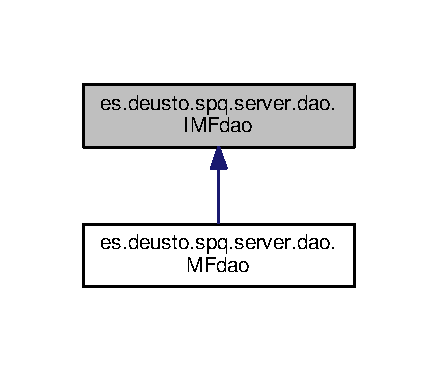
\includegraphics[width=210pt]{interfacees_1_1deusto_1_1spq_1_1server_1_1dao_1_1_i_m_fdao__inherit__graph}
\end{center}
\end{figure}
\subsection*{Public Member Functions}
\begin{DoxyCompactItemize}
\item 
boolean \hyperlink{interfacees_1_1deusto_1_1spq_1_1server_1_1dao_1_1_i_m_fdao_a3106afd4fe9bbf720f98c8a8c4a9f433}{store\+User} (\hyperlink{classes_1_1deusto_1_1spq_1_1server_1_1data_1_1_usuario}{Usuario} u)
\item 
boolean \hyperlink{interfacees_1_1deusto_1_1spq_1_1server_1_1dao_1_1_i_m_fdao_abc85b827eab8794bd6e00f1df9cf156d}{login\+User} (String email, String password)
\item 
String \hyperlink{interfacees_1_1deusto_1_1spq_1_1server_1_1dao_1_1_i_m_fdao_a1a090e575d74774692844b5543320fc4}{get\+User\+Name} ()
\item 
void \hyperlink{interfacees_1_1deusto_1_1spq_1_1server_1_1dao_1_1_i_m_fdao_a8d0676aebfd63e2bd07ab7a6ff8e7571}{store\+Song} (\hyperlink{classes_1_1deusto_1_1spq_1_1server_1_1data_1_1_cancion}{Cancion} c)
\item 
String \hyperlink{interfacees_1_1deusto_1_1spq_1_1server_1_1dao_1_1_i_m_fdao_acd2152ac1a19753c426b0a0e32dc3e47}{get\+User\+Mail} ()
\item 
List$<$ String $>$ \hyperlink{interfacees_1_1deusto_1_1spq_1_1server_1_1dao_1_1_i_m_fdao_a365443ee24a364f5b4824318ed90af6d}{search\+Song} (String keyword)
\item 
List$<$ String $>$ \hyperlink{interfacees_1_1deusto_1_1spq_1_1server_1_1dao_1_1_i_m_fdao_a2dbfe3fad8b76ecf116fc3411b3280d5}{load\+Songs} ()
\item 
boolean \hyperlink{interfacees_1_1deusto_1_1spq_1_1server_1_1dao_1_1_i_m_fdao_a2babd39655f8a57f0b64d3bd912e3215}{check\+User} (\hyperlink{classes_1_1deusto_1_1spq_1_1server_1_1data_1_1_usuario}{Usuario} user)
\end{DoxyCompactItemize}


\subsection{Detailed Description}


Definition at line 8 of file I\+M\+Fdao.\+java.



\subsection{Member Function Documentation}
\index{es\+::deusto\+::spq\+::server\+::dao\+::\+I\+M\+Fdao@{es\+::deusto\+::spq\+::server\+::dao\+::\+I\+M\+Fdao}!check\+User@{check\+User}}
\index{check\+User@{check\+User}!es\+::deusto\+::spq\+::server\+::dao\+::\+I\+M\+Fdao@{es\+::deusto\+::spq\+::server\+::dao\+::\+I\+M\+Fdao}}
\subsubsection[{\texorpdfstring{check\+User(\+Usuario user)}{checkUser(Usuario user)}}]{\setlength{\rightskip}{0pt plus 5cm}boolean es.\+deusto.\+spq.\+server.\+dao.\+I\+M\+Fdao.\+check\+User (
\begin{DoxyParamCaption}
\item[{{\bf Usuario}}]{user}
\end{DoxyParamCaption}
)}\hypertarget{interfacees_1_1deusto_1_1spq_1_1server_1_1dao_1_1_i_m_fdao_a2babd39655f8a57f0b64d3bd912e3215}{}\label{interfacees_1_1deusto_1_1spq_1_1server_1_1dao_1_1_i_m_fdao_a2babd39655f8a57f0b64d3bd912e3215}

\begin{DoxyParams}{Parameters}
{\em user} & \\
\hline
\end{DoxyParams}
\begin{DoxyReturn}{Returns}

\end{DoxyReturn}


Implemented in \hyperlink{classes_1_1deusto_1_1spq_1_1server_1_1dao_1_1_m_fdao_aa63ea4816fac392840181fb557bf485c}{es.\+deusto.\+spq.\+server.\+dao.\+M\+Fdao}.

\index{es\+::deusto\+::spq\+::server\+::dao\+::\+I\+M\+Fdao@{es\+::deusto\+::spq\+::server\+::dao\+::\+I\+M\+Fdao}!get\+User\+Mail@{get\+User\+Mail}}
\index{get\+User\+Mail@{get\+User\+Mail}!es\+::deusto\+::spq\+::server\+::dao\+::\+I\+M\+Fdao@{es\+::deusto\+::spq\+::server\+::dao\+::\+I\+M\+Fdao}}
\subsubsection[{\texorpdfstring{get\+User\+Mail()}{getUserMail()}}]{\setlength{\rightskip}{0pt plus 5cm}String es.\+deusto.\+spq.\+server.\+dao.\+I\+M\+Fdao.\+get\+User\+Mail (
\begin{DoxyParamCaption}
{}
\end{DoxyParamCaption}
)}\hypertarget{interfacees_1_1deusto_1_1spq_1_1server_1_1dao_1_1_i_m_fdao_acd2152ac1a19753c426b0a0e32dc3e47}{}\label{interfacees_1_1deusto_1_1spq_1_1server_1_1dao_1_1_i_m_fdao_acd2152ac1a19753c426b0a0e32dc3e47}
\begin{DoxyReturn}{Returns}

\end{DoxyReturn}


Implemented in \hyperlink{classes_1_1deusto_1_1spq_1_1server_1_1dao_1_1_m_fdao_a765a8fa4b291fec932c56c0549adea9a}{es.\+deusto.\+spq.\+server.\+dao.\+M\+Fdao}.



Here is the caller graph for this function\+:\nopagebreak
\begin{figure}[H]
\begin{center}
\leavevmode
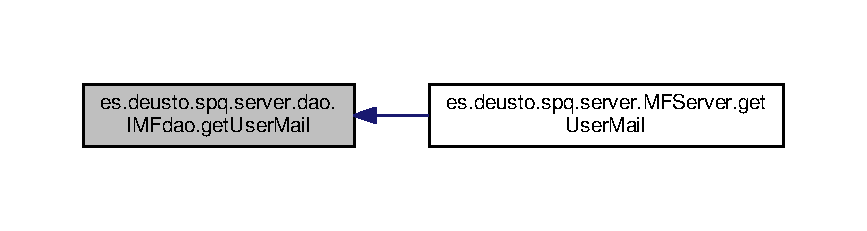
\includegraphics[width=350pt]{interfacees_1_1deusto_1_1spq_1_1server_1_1dao_1_1_i_m_fdao_acd2152ac1a19753c426b0a0e32dc3e47_icgraph}
\end{center}
\end{figure}


\index{es\+::deusto\+::spq\+::server\+::dao\+::\+I\+M\+Fdao@{es\+::deusto\+::spq\+::server\+::dao\+::\+I\+M\+Fdao}!get\+User\+Name@{get\+User\+Name}}
\index{get\+User\+Name@{get\+User\+Name}!es\+::deusto\+::spq\+::server\+::dao\+::\+I\+M\+Fdao@{es\+::deusto\+::spq\+::server\+::dao\+::\+I\+M\+Fdao}}
\subsubsection[{\texorpdfstring{get\+User\+Name()}{getUserName()}}]{\setlength{\rightskip}{0pt plus 5cm}String es.\+deusto.\+spq.\+server.\+dao.\+I\+M\+Fdao.\+get\+User\+Name (
\begin{DoxyParamCaption}
{}
\end{DoxyParamCaption}
)}\hypertarget{interfacees_1_1deusto_1_1spq_1_1server_1_1dao_1_1_i_m_fdao_a1a090e575d74774692844b5543320fc4}{}\label{interfacees_1_1deusto_1_1spq_1_1server_1_1dao_1_1_i_m_fdao_a1a090e575d74774692844b5543320fc4}
\begin{DoxyReturn}{Returns}

\end{DoxyReturn}


Implemented in \hyperlink{classes_1_1deusto_1_1spq_1_1server_1_1dao_1_1_m_fdao_af351618006ddba9fcf450f5288808020}{es.\+deusto.\+spq.\+server.\+dao.\+M\+Fdao}.



Here is the caller graph for this function\+:\nopagebreak
\begin{figure}[H]
\begin{center}
\leavevmode
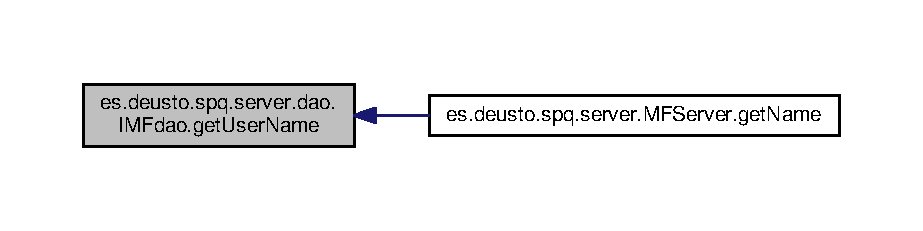
\includegraphics[width=350pt]{interfacees_1_1deusto_1_1spq_1_1server_1_1dao_1_1_i_m_fdao_a1a090e575d74774692844b5543320fc4_icgraph}
\end{center}
\end{figure}


\index{es\+::deusto\+::spq\+::server\+::dao\+::\+I\+M\+Fdao@{es\+::deusto\+::spq\+::server\+::dao\+::\+I\+M\+Fdao}!load\+Songs@{load\+Songs}}
\index{load\+Songs@{load\+Songs}!es\+::deusto\+::spq\+::server\+::dao\+::\+I\+M\+Fdao@{es\+::deusto\+::spq\+::server\+::dao\+::\+I\+M\+Fdao}}
\subsubsection[{\texorpdfstring{load\+Songs()}{loadSongs()}}]{\setlength{\rightskip}{0pt plus 5cm}List$<$String$>$ es.\+deusto.\+spq.\+server.\+dao.\+I\+M\+Fdao.\+load\+Songs (
\begin{DoxyParamCaption}
{}
\end{DoxyParamCaption}
)}\hypertarget{interfacees_1_1deusto_1_1spq_1_1server_1_1dao_1_1_i_m_fdao_a2dbfe3fad8b76ecf116fc3411b3280d5}{}\label{interfacees_1_1deusto_1_1spq_1_1server_1_1dao_1_1_i_m_fdao_a2dbfe3fad8b76ecf116fc3411b3280d5}
\begin{DoxyReturn}{Returns}

\end{DoxyReturn}


Implemented in \hyperlink{classes_1_1deusto_1_1spq_1_1server_1_1dao_1_1_m_fdao_ab5e0871df69651fdb41d03cdc4cfc25b}{es.\+deusto.\+spq.\+server.\+dao.\+M\+Fdao}.



Here is the caller graph for this function\+:\nopagebreak
\begin{figure}[H]
\begin{center}
\leavevmode
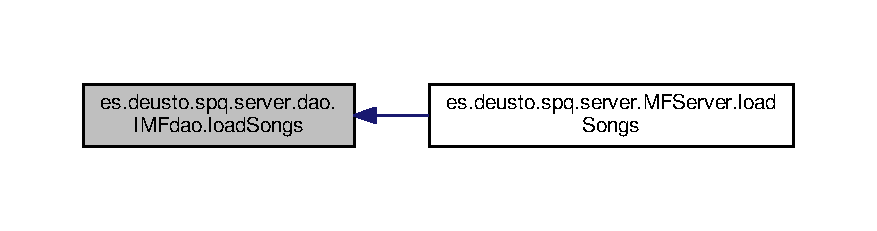
\includegraphics[width=350pt]{interfacees_1_1deusto_1_1spq_1_1server_1_1dao_1_1_i_m_fdao_a2dbfe3fad8b76ecf116fc3411b3280d5_icgraph}
\end{center}
\end{figure}


\index{es\+::deusto\+::spq\+::server\+::dao\+::\+I\+M\+Fdao@{es\+::deusto\+::spq\+::server\+::dao\+::\+I\+M\+Fdao}!login\+User@{login\+User}}
\index{login\+User@{login\+User}!es\+::deusto\+::spq\+::server\+::dao\+::\+I\+M\+Fdao@{es\+::deusto\+::spq\+::server\+::dao\+::\+I\+M\+Fdao}}
\subsubsection[{\texorpdfstring{login\+User(\+String email, String password)}{loginUser(String email, String password)}}]{\setlength{\rightskip}{0pt plus 5cm}boolean es.\+deusto.\+spq.\+server.\+dao.\+I\+M\+Fdao.\+login\+User (
\begin{DoxyParamCaption}
\item[{String}]{email, }
\item[{String}]{password}
\end{DoxyParamCaption}
)}\hypertarget{interfacees_1_1deusto_1_1spq_1_1server_1_1dao_1_1_i_m_fdao_abc85b827eab8794bd6e00f1df9cf156d}{}\label{interfacees_1_1deusto_1_1spq_1_1server_1_1dao_1_1_i_m_fdao_abc85b827eab8794bd6e00f1df9cf156d}

\begin{DoxyParams}{Parameters}
{\em email} & \\
\hline
{\em password} & \\
\hline
\end{DoxyParams}
\begin{DoxyReturn}{Returns}

\end{DoxyReturn}


Implemented in \hyperlink{classes_1_1deusto_1_1spq_1_1server_1_1dao_1_1_m_fdao_a1444b8fec0c62d8edcccdee255b07457}{es.\+deusto.\+spq.\+server.\+dao.\+M\+Fdao}.



Here is the caller graph for this function\+:\nopagebreak
\begin{figure}[H]
\begin{center}
\leavevmode
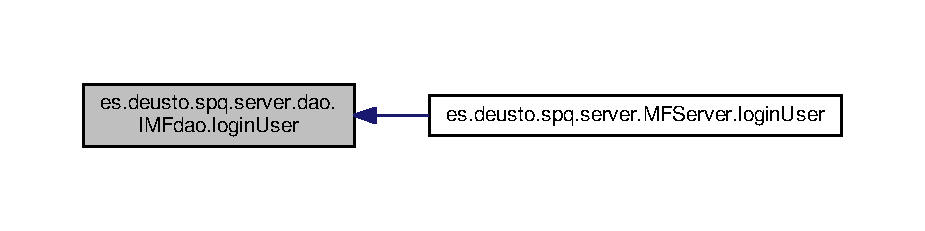
\includegraphics[width=350pt]{interfacees_1_1deusto_1_1spq_1_1server_1_1dao_1_1_i_m_fdao_abc85b827eab8794bd6e00f1df9cf156d_icgraph}
\end{center}
\end{figure}


\index{es\+::deusto\+::spq\+::server\+::dao\+::\+I\+M\+Fdao@{es\+::deusto\+::spq\+::server\+::dao\+::\+I\+M\+Fdao}!search\+Song@{search\+Song}}
\index{search\+Song@{search\+Song}!es\+::deusto\+::spq\+::server\+::dao\+::\+I\+M\+Fdao@{es\+::deusto\+::spq\+::server\+::dao\+::\+I\+M\+Fdao}}
\subsubsection[{\texorpdfstring{search\+Song(\+String keyword)}{searchSong(String keyword)}}]{\setlength{\rightskip}{0pt plus 5cm}List$<$String$>$ es.\+deusto.\+spq.\+server.\+dao.\+I\+M\+Fdao.\+search\+Song (
\begin{DoxyParamCaption}
\item[{String}]{keyword}
\end{DoxyParamCaption}
)}\hypertarget{interfacees_1_1deusto_1_1spq_1_1server_1_1dao_1_1_i_m_fdao_a365443ee24a364f5b4824318ed90af6d}{}\label{interfacees_1_1deusto_1_1spq_1_1server_1_1dao_1_1_i_m_fdao_a365443ee24a364f5b4824318ed90af6d}

\begin{DoxyParams}{Parameters}
{\em keyword} & \\
\hline
\end{DoxyParams}
\begin{DoxyReturn}{Returns}

\end{DoxyReturn}


Implemented in \hyperlink{classes_1_1deusto_1_1spq_1_1server_1_1dao_1_1_m_fdao_a69b3efd8be9b8a2add7d57f703a8f4d7}{es.\+deusto.\+spq.\+server.\+dao.\+M\+Fdao}.



Here is the caller graph for this function\+:\nopagebreak
\begin{figure}[H]
\begin{center}
\leavevmode
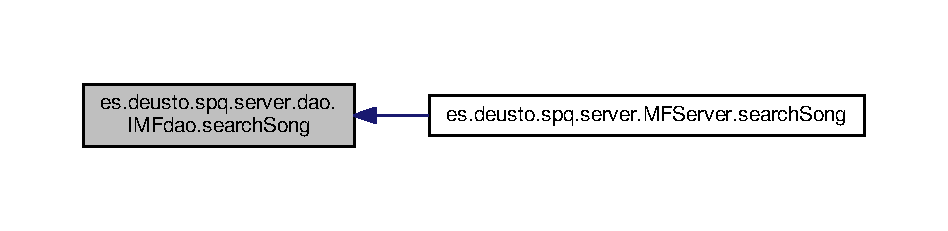
\includegraphics[width=350pt]{interfacees_1_1deusto_1_1spq_1_1server_1_1dao_1_1_i_m_fdao_a365443ee24a364f5b4824318ed90af6d_icgraph}
\end{center}
\end{figure}


\index{es\+::deusto\+::spq\+::server\+::dao\+::\+I\+M\+Fdao@{es\+::deusto\+::spq\+::server\+::dao\+::\+I\+M\+Fdao}!store\+Song@{store\+Song}}
\index{store\+Song@{store\+Song}!es\+::deusto\+::spq\+::server\+::dao\+::\+I\+M\+Fdao@{es\+::deusto\+::spq\+::server\+::dao\+::\+I\+M\+Fdao}}
\subsubsection[{\texorpdfstring{store\+Song(\+Cancion c)}{storeSong(Cancion c)}}]{\setlength{\rightskip}{0pt plus 5cm}void es.\+deusto.\+spq.\+server.\+dao.\+I\+M\+Fdao.\+store\+Song (
\begin{DoxyParamCaption}
\item[{{\bf Cancion}}]{c}
\end{DoxyParamCaption}
)}\hypertarget{interfacees_1_1deusto_1_1spq_1_1server_1_1dao_1_1_i_m_fdao_a8d0676aebfd63e2bd07ab7a6ff8e7571}{}\label{interfacees_1_1deusto_1_1spq_1_1server_1_1dao_1_1_i_m_fdao_a8d0676aebfd63e2bd07ab7a6ff8e7571}

\begin{DoxyParams}{Parameters}
{\em c} & \\
\hline
\end{DoxyParams}


Implemented in \hyperlink{classes_1_1deusto_1_1spq_1_1server_1_1dao_1_1_m_fdao_a4e8d7b5135ed5c9ccb65b6cc499c7278}{es.\+deusto.\+spq.\+server.\+dao.\+M\+Fdao}.



Here is the caller graph for this function\+:\nopagebreak
\begin{figure}[H]
\begin{center}
\leavevmode
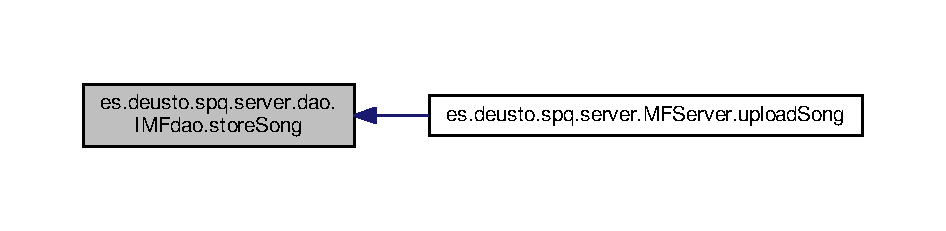
\includegraphics[width=350pt]{interfacees_1_1deusto_1_1spq_1_1server_1_1dao_1_1_i_m_fdao_a8d0676aebfd63e2bd07ab7a6ff8e7571_icgraph}
\end{center}
\end{figure}


\index{es\+::deusto\+::spq\+::server\+::dao\+::\+I\+M\+Fdao@{es\+::deusto\+::spq\+::server\+::dao\+::\+I\+M\+Fdao}!store\+User@{store\+User}}
\index{store\+User@{store\+User}!es\+::deusto\+::spq\+::server\+::dao\+::\+I\+M\+Fdao@{es\+::deusto\+::spq\+::server\+::dao\+::\+I\+M\+Fdao}}
\subsubsection[{\texorpdfstring{store\+User(\+Usuario u)}{storeUser(Usuario u)}}]{\setlength{\rightskip}{0pt plus 5cm}boolean es.\+deusto.\+spq.\+server.\+dao.\+I\+M\+Fdao.\+store\+User (
\begin{DoxyParamCaption}
\item[{{\bf Usuario}}]{u}
\end{DoxyParamCaption}
)}\hypertarget{interfacees_1_1deusto_1_1spq_1_1server_1_1dao_1_1_i_m_fdao_a3106afd4fe9bbf720f98c8a8c4a9f433}{}\label{interfacees_1_1deusto_1_1spq_1_1server_1_1dao_1_1_i_m_fdao_a3106afd4fe9bbf720f98c8a8c4a9f433}

\begin{DoxyParams}{Parameters}
{\em u} & \\
\hline
\end{DoxyParams}
\begin{DoxyReturn}{Returns}

\end{DoxyReturn}


Implemented in \hyperlink{classes_1_1deusto_1_1spq_1_1server_1_1dao_1_1_m_fdao_a018654ad3063099187b0005145a36ce6}{es.\+deusto.\+spq.\+server.\+dao.\+M\+Fdao}.



Here is the caller graph for this function\+:\nopagebreak
\begin{figure}[H]
\begin{center}
\leavevmode
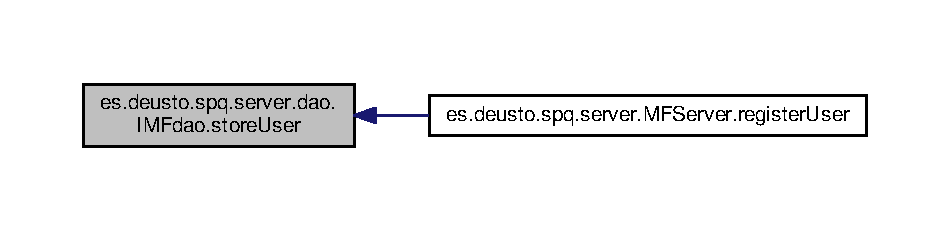
\includegraphics[width=350pt]{interfacees_1_1deusto_1_1spq_1_1server_1_1dao_1_1_i_m_fdao_a3106afd4fe9bbf720f98c8a8c4a9f433_icgraph}
\end{center}
\end{figure}




The documentation for this interface was generated from the following file\+:\begin{DoxyCompactItemize}
\item 
src/main/java/es/deusto/spq/server/dao/\hyperlink{_i_m_fdao_8java}{I\+M\+Fdao.\+java}\end{DoxyCompactItemize}

\hypertarget{interfacees_1_1deusto_1_1spq_1_1server_1_1_i_m_f_server}{}\section{es.\+deusto.\+spq.\+server.\+I\+M\+F\+Server Interface Reference}
\label{interfacees_1_1deusto_1_1spq_1_1server_1_1_i_m_f_server}\index{es.\+deusto.\+spq.\+server.\+I\+M\+F\+Server@{es.\+deusto.\+spq.\+server.\+I\+M\+F\+Server}}


Inheritance diagram for es.\+deusto.\+spq.\+server.\+I\+M\+F\+Server\+:\nopagebreak
\begin{figure}[H]
\begin{center}
\leavevmode
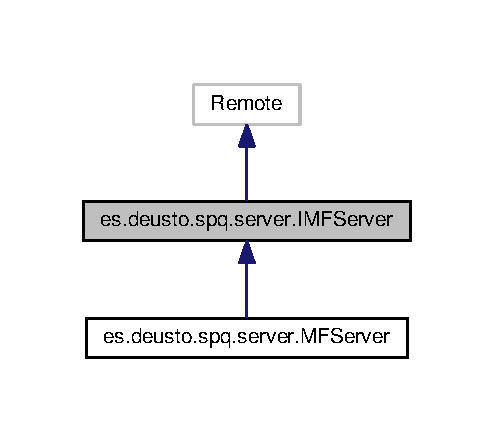
\includegraphics[width=237pt]{interfacees_1_1deusto_1_1spq_1_1server_1_1_i_m_f_server__inherit__graph}
\end{center}
\end{figure}


Collaboration diagram for es.\+deusto.\+spq.\+server.\+I\+M\+F\+Server\+:\nopagebreak
\begin{figure}[H]
\begin{center}
\leavevmode
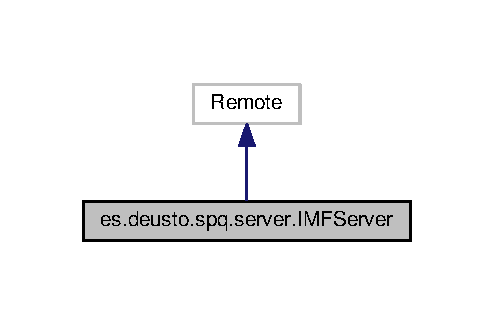
\includegraphics[width=237pt]{interfacees_1_1deusto_1_1spq_1_1server_1_1_i_m_f_server__coll__graph}
\end{center}
\end{figure}
\subsection*{Public Member Functions}
\begin{DoxyCompactItemize}
\item 
String \hyperlink{interfacees_1_1deusto_1_1spq_1_1server_1_1_i_m_f_server_a368aca60ea2ccba7951fc7e3594b7368}{say\+Message} (String login, String password, String message)  throws Remote\+Exception
\item 
boolean \hyperlink{interfacees_1_1deusto_1_1spq_1_1server_1_1_i_m_f_server_a51f1f5ea155f4f33ce02d39f7ab9696b}{register\+User} (String nombre, String apellido, String email, String password)  throws Remote\+Exception
\item 
boolean \hyperlink{interfacees_1_1deusto_1_1spq_1_1server_1_1_i_m_f_server_afb6983f4de78858b8e73e8f55596374d}{login\+User} (String email, String password)  throws Remote\+Exception
\item 
String \hyperlink{interfacees_1_1deusto_1_1spq_1_1server_1_1_i_m_f_server_aa5653bb7aa1be80a2d94ebd5785ea409}{get\+Name} ()  throws Remote\+Exception
\item 
String \hyperlink{interfacees_1_1deusto_1_1spq_1_1server_1_1_i_m_f_server_a009e437ac332036c21d01ceccc217526}{get\+User\+Mail} ()  throws Remote\+Exception
\item 
List$<$ String $>$ \hyperlink{interfacees_1_1deusto_1_1spq_1_1server_1_1_i_m_f_server_a3a6e5481a3cc2f543c3ef1e90e4e7da6}{load\+Songs} ()  throws Remote\+Exception
\item 
List$<$ String $>$ \hyperlink{interfacees_1_1deusto_1_1spq_1_1server_1_1_i_m_f_server_a4b469cde52367aeb852ff5959ab47bf5}{search\+Song} (String keyword)  throws Remote\+Exception
\item 
void \hyperlink{interfacees_1_1deusto_1_1spq_1_1server_1_1_i_m_f_server_ad1c6aec7730ce9a49c61afdc79a9e740}{upload\+Song} (String name, String genero, String artista, String cancion, String useridentification)  throws Remote\+Exception
\end{DoxyCompactItemize}


\subsection{Detailed Description}


Definition at line 9 of file I\+M\+F\+Server.\+java.



\subsection{Member Function Documentation}
\index{es\+::deusto\+::spq\+::server\+::\+I\+M\+F\+Server@{es\+::deusto\+::spq\+::server\+::\+I\+M\+F\+Server}!get\+Name@{get\+Name}}
\index{get\+Name@{get\+Name}!es\+::deusto\+::spq\+::server\+::\+I\+M\+F\+Server@{es\+::deusto\+::spq\+::server\+::\+I\+M\+F\+Server}}
\subsubsection[{\texorpdfstring{get\+Name()}{getName()}}]{\setlength{\rightskip}{0pt plus 5cm}String es.\+deusto.\+spq.\+server.\+I\+M\+F\+Server.\+get\+Name (
\begin{DoxyParamCaption}
{}
\end{DoxyParamCaption}
) throws Remote\+Exception}\hypertarget{interfacees_1_1deusto_1_1spq_1_1server_1_1_i_m_f_server_aa5653bb7aa1be80a2d94ebd5785ea409}{}\label{interfacees_1_1deusto_1_1spq_1_1server_1_1_i_m_f_server_aa5653bb7aa1be80a2d94ebd5785ea409}


Implemented in \hyperlink{classes_1_1deusto_1_1spq_1_1server_1_1_m_f_server_a75eaf5cc57e286889d322248a83a9418}{es.\+deusto.\+spq.\+server.\+M\+F\+Server}.



Here is the caller graph for this function\+:\nopagebreak
\begin{figure}[H]
\begin{center}
\leavevmode
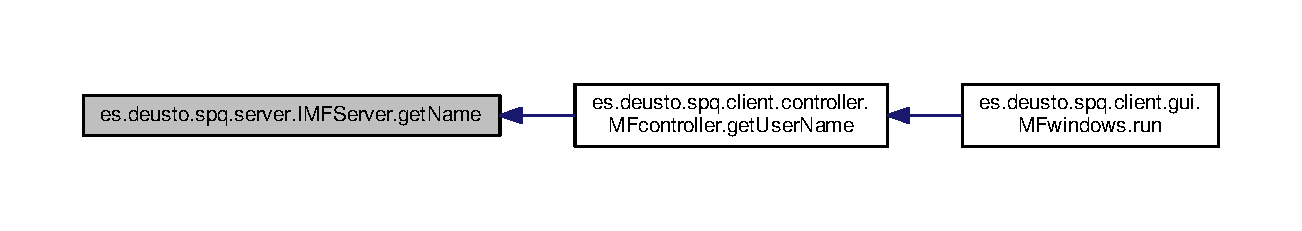
\includegraphics[width=350pt]{interfacees_1_1deusto_1_1spq_1_1server_1_1_i_m_f_server_aa5653bb7aa1be80a2d94ebd5785ea409_icgraph}
\end{center}
\end{figure}


\index{es\+::deusto\+::spq\+::server\+::\+I\+M\+F\+Server@{es\+::deusto\+::spq\+::server\+::\+I\+M\+F\+Server}!get\+User\+Mail@{get\+User\+Mail}}
\index{get\+User\+Mail@{get\+User\+Mail}!es\+::deusto\+::spq\+::server\+::\+I\+M\+F\+Server@{es\+::deusto\+::spq\+::server\+::\+I\+M\+F\+Server}}
\subsubsection[{\texorpdfstring{get\+User\+Mail()}{getUserMail()}}]{\setlength{\rightskip}{0pt plus 5cm}String es.\+deusto.\+spq.\+server.\+I\+M\+F\+Server.\+get\+User\+Mail (
\begin{DoxyParamCaption}
{}
\end{DoxyParamCaption}
) throws Remote\+Exception}\hypertarget{interfacees_1_1deusto_1_1spq_1_1server_1_1_i_m_f_server_a009e437ac332036c21d01ceccc217526}{}\label{interfacees_1_1deusto_1_1spq_1_1server_1_1_i_m_f_server_a009e437ac332036c21d01ceccc217526}


Implemented in \hyperlink{classes_1_1deusto_1_1spq_1_1server_1_1_m_f_server_a01d5a6424526e32d8e8ace58776ccad4}{es.\+deusto.\+spq.\+server.\+M\+F\+Server}.



Here is the caller graph for this function\+:\nopagebreak
\begin{figure}[H]
\begin{center}
\leavevmode
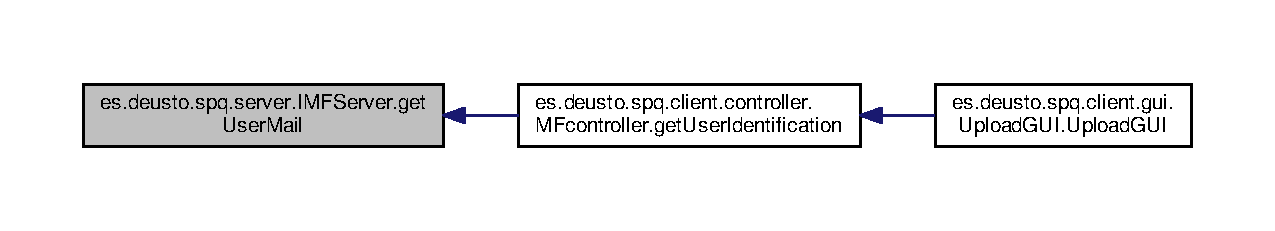
\includegraphics[width=350pt]{interfacees_1_1deusto_1_1spq_1_1server_1_1_i_m_f_server_a009e437ac332036c21d01ceccc217526_icgraph}
\end{center}
\end{figure}


\index{es\+::deusto\+::spq\+::server\+::\+I\+M\+F\+Server@{es\+::deusto\+::spq\+::server\+::\+I\+M\+F\+Server}!load\+Songs@{load\+Songs}}
\index{load\+Songs@{load\+Songs}!es\+::deusto\+::spq\+::server\+::\+I\+M\+F\+Server@{es\+::deusto\+::spq\+::server\+::\+I\+M\+F\+Server}}
\subsubsection[{\texorpdfstring{load\+Songs()}{loadSongs()}}]{\setlength{\rightskip}{0pt plus 5cm}List$<$String$>$ es.\+deusto.\+spq.\+server.\+I\+M\+F\+Server.\+load\+Songs (
\begin{DoxyParamCaption}
{}
\end{DoxyParamCaption}
) throws Remote\+Exception}\hypertarget{interfacees_1_1deusto_1_1spq_1_1server_1_1_i_m_f_server_a3a6e5481a3cc2f543c3ef1e90e4e7da6}{}\label{interfacees_1_1deusto_1_1spq_1_1server_1_1_i_m_f_server_a3a6e5481a3cc2f543c3ef1e90e4e7da6}


Implemented in \hyperlink{classes_1_1deusto_1_1spq_1_1server_1_1_m_f_server_ae2c8a121696577c33472b1bad368a1df}{es.\+deusto.\+spq.\+server.\+M\+F\+Server}.



Here is the caller graph for this function\+:\nopagebreak
\begin{figure}[H]
\begin{center}
\leavevmode
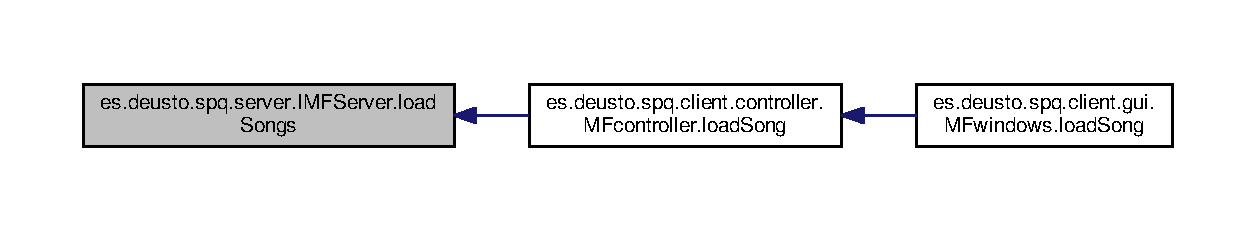
\includegraphics[width=350pt]{interfacees_1_1deusto_1_1spq_1_1server_1_1_i_m_f_server_a3a6e5481a3cc2f543c3ef1e90e4e7da6_icgraph}
\end{center}
\end{figure}


\index{es\+::deusto\+::spq\+::server\+::\+I\+M\+F\+Server@{es\+::deusto\+::spq\+::server\+::\+I\+M\+F\+Server}!login\+User@{login\+User}}
\index{login\+User@{login\+User}!es\+::deusto\+::spq\+::server\+::\+I\+M\+F\+Server@{es\+::deusto\+::spq\+::server\+::\+I\+M\+F\+Server}}
\subsubsection[{\texorpdfstring{login\+User(\+String email, String password)}{loginUser(String email, String password)}}]{\setlength{\rightskip}{0pt plus 5cm}boolean es.\+deusto.\+spq.\+server.\+I\+M\+F\+Server.\+login\+User (
\begin{DoxyParamCaption}
\item[{String}]{email, }
\item[{String}]{password}
\end{DoxyParamCaption}
) throws Remote\+Exception}\hypertarget{interfacees_1_1deusto_1_1spq_1_1server_1_1_i_m_f_server_afb6983f4de78858b8e73e8f55596374d}{}\label{interfacees_1_1deusto_1_1spq_1_1server_1_1_i_m_f_server_afb6983f4de78858b8e73e8f55596374d}


Implemented in \hyperlink{classes_1_1deusto_1_1spq_1_1server_1_1_m_f_server_ad242cbf142dbea245a4be10f52b16745}{es.\+deusto.\+spq.\+server.\+M\+F\+Server}.



Here is the caller graph for this function\+:\nopagebreak
\begin{figure}[H]
\begin{center}
\leavevmode
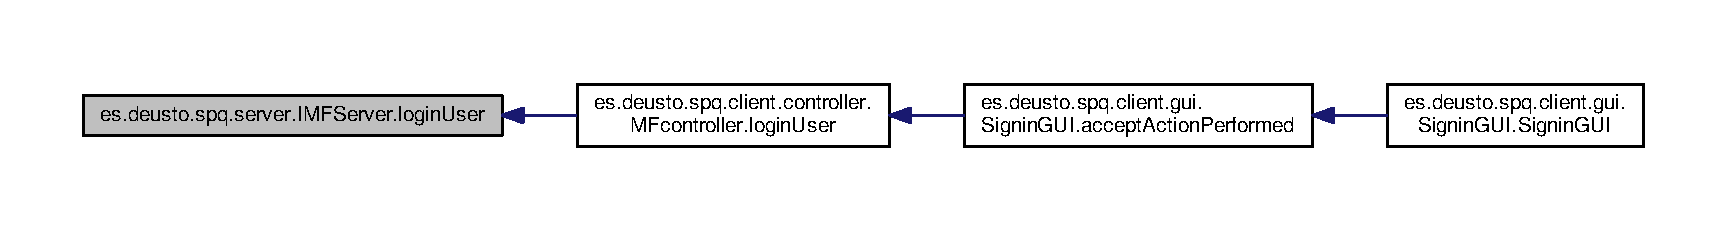
\includegraphics[width=350pt]{interfacees_1_1deusto_1_1spq_1_1server_1_1_i_m_f_server_afb6983f4de78858b8e73e8f55596374d_icgraph}
\end{center}
\end{figure}


\index{es\+::deusto\+::spq\+::server\+::\+I\+M\+F\+Server@{es\+::deusto\+::spq\+::server\+::\+I\+M\+F\+Server}!register\+User@{register\+User}}
\index{register\+User@{register\+User}!es\+::deusto\+::spq\+::server\+::\+I\+M\+F\+Server@{es\+::deusto\+::spq\+::server\+::\+I\+M\+F\+Server}}
\subsubsection[{\texorpdfstring{register\+User(\+String nombre, String apellido, String email, String password)}{registerUser(String nombre, String apellido, String email, String password)}}]{\setlength{\rightskip}{0pt plus 5cm}boolean es.\+deusto.\+spq.\+server.\+I\+M\+F\+Server.\+register\+User (
\begin{DoxyParamCaption}
\item[{String}]{nombre, }
\item[{String}]{apellido, }
\item[{String}]{email, }
\item[{String}]{password}
\end{DoxyParamCaption}
) throws Remote\+Exception}\hypertarget{interfacees_1_1deusto_1_1spq_1_1server_1_1_i_m_f_server_a51f1f5ea155f4f33ce02d39f7ab9696b}{}\label{interfacees_1_1deusto_1_1spq_1_1server_1_1_i_m_f_server_a51f1f5ea155f4f33ce02d39f7ab9696b}


Implemented in \hyperlink{classes_1_1deusto_1_1spq_1_1server_1_1_m_f_server_abf0e32da4f876c11c864593f5d7e39f2}{es.\+deusto.\+spq.\+server.\+M\+F\+Server}.



Here is the caller graph for this function\+:\nopagebreak
\begin{figure}[H]
\begin{center}
\leavevmode
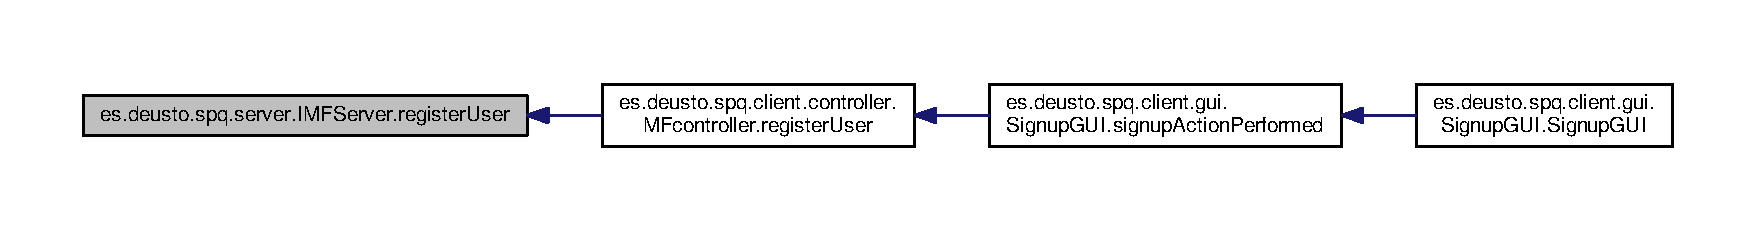
\includegraphics[width=350pt]{interfacees_1_1deusto_1_1spq_1_1server_1_1_i_m_f_server_a51f1f5ea155f4f33ce02d39f7ab9696b_icgraph}
\end{center}
\end{figure}


\index{es\+::deusto\+::spq\+::server\+::\+I\+M\+F\+Server@{es\+::deusto\+::spq\+::server\+::\+I\+M\+F\+Server}!say\+Message@{say\+Message}}
\index{say\+Message@{say\+Message}!es\+::deusto\+::spq\+::server\+::\+I\+M\+F\+Server@{es\+::deusto\+::spq\+::server\+::\+I\+M\+F\+Server}}
\subsubsection[{\texorpdfstring{say\+Message(\+String login, String password, String message)}{sayMessage(String login, String password, String message)}}]{\setlength{\rightskip}{0pt plus 5cm}String es.\+deusto.\+spq.\+server.\+I\+M\+F\+Server.\+say\+Message (
\begin{DoxyParamCaption}
\item[{String}]{login, }
\item[{String}]{password, }
\item[{String}]{message}
\end{DoxyParamCaption}
) throws Remote\+Exception}\hypertarget{interfacees_1_1deusto_1_1spq_1_1server_1_1_i_m_f_server_a368aca60ea2ccba7951fc7e3594b7368}{}\label{interfacees_1_1deusto_1_1spq_1_1server_1_1_i_m_f_server_a368aca60ea2ccba7951fc7e3594b7368}


Implemented in \hyperlink{classes_1_1deusto_1_1spq_1_1server_1_1_m_f_server_a8d8a50dc58a3b1bd821b95fd30f64af5}{es.\+deusto.\+spq.\+server.\+M\+F\+Server}.

\index{es\+::deusto\+::spq\+::server\+::\+I\+M\+F\+Server@{es\+::deusto\+::spq\+::server\+::\+I\+M\+F\+Server}!search\+Song@{search\+Song}}
\index{search\+Song@{search\+Song}!es\+::deusto\+::spq\+::server\+::\+I\+M\+F\+Server@{es\+::deusto\+::spq\+::server\+::\+I\+M\+F\+Server}}
\subsubsection[{\texorpdfstring{search\+Song(\+String keyword)}{searchSong(String keyword)}}]{\setlength{\rightskip}{0pt plus 5cm}List$<$String$>$ es.\+deusto.\+spq.\+server.\+I\+M\+F\+Server.\+search\+Song (
\begin{DoxyParamCaption}
\item[{String}]{keyword}
\end{DoxyParamCaption}
) throws Remote\+Exception}\hypertarget{interfacees_1_1deusto_1_1spq_1_1server_1_1_i_m_f_server_a4b469cde52367aeb852ff5959ab47bf5}{}\label{interfacees_1_1deusto_1_1spq_1_1server_1_1_i_m_f_server_a4b469cde52367aeb852ff5959ab47bf5}


Implemented in \hyperlink{classes_1_1deusto_1_1spq_1_1server_1_1_m_f_server_ac317c84d14b002d8446046df9345c7ab}{es.\+deusto.\+spq.\+server.\+M\+F\+Server}.



Here is the caller graph for this function\+:\nopagebreak
\begin{figure}[H]
\begin{center}
\leavevmode
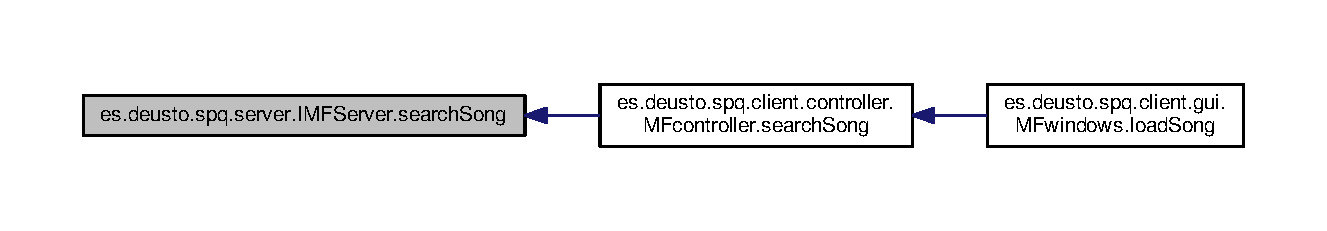
\includegraphics[width=350pt]{interfacees_1_1deusto_1_1spq_1_1server_1_1_i_m_f_server_a4b469cde52367aeb852ff5959ab47bf5_icgraph}
\end{center}
\end{figure}


\index{es\+::deusto\+::spq\+::server\+::\+I\+M\+F\+Server@{es\+::deusto\+::spq\+::server\+::\+I\+M\+F\+Server}!upload\+Song@{upload\+Song}}
\index{upload\+Song@{upload\+Song}!es\+::deusto\+::spq\+::server\+::\+I\+M\+F\+Server@{es\+::deusto\+::spq\+::server\+::\+I\+M\+F\+Server}}
\subsubsection[{\texorpdfstring{upload\+Song(\+String name, String genero, String artista, String cancion, String useridentification)}{uploadSong(String name, String genero, String artista, String cancion, String useridentification)}}]{\setlength{\rightskip}{0pt plus 5cm}void es.\+deusto.\+spq.\+server.\+I\+M\+F\+Server.\+upload\+Song (
\begin{DoxyParamCaption}
\item[{String}]{name, }
\item[{String}]{genero, }
\item[{String}]{artista, }
\item[{String}]{cancion, }
\item[{String}]{useridentification}
\end{DoxyParamCaption}
) throws Remote\+Exception}\hypertarget{interfacees_1_1deusto_1_1spq_1_1server_1_1_i_m_f_server_ad1c6aec7730ce9a49c61afdc79a9e740}{}\label{interfacees_1_1deusto_1_1spq_1_1server_1_1_i_m_f_server_ad1c6aec7730ce9a49c61afdc79a9e740}


Implemented in \hyperlink{classes_1_1deusto_1_1spq_1_1server_1_1_m_f_server_a6bd9178166f1294c83144ee792b15cf3}{es.\+deusto.\+spq.\+server.\+M\+F\+Server}.



Here is the caller graph for this function\+:\nopagebreak
\begin{figure}[H]
\begin{center}
\leavevmode
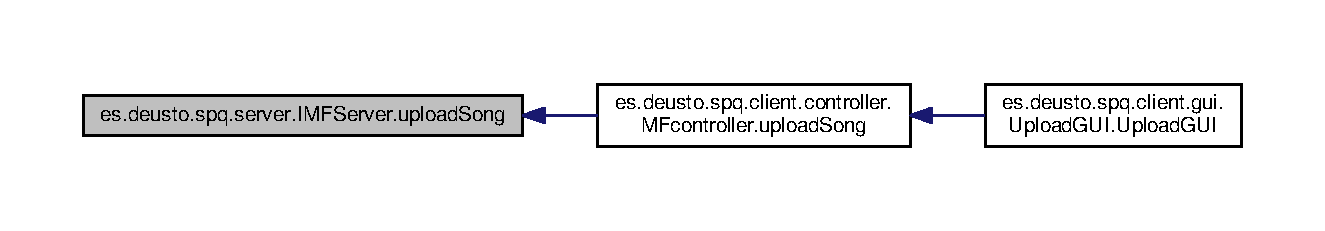
\includegraphics[width=350pt]{interfacees_1_1deusto_1_1spq_1_1server_1_1_i_m_f_server_ad1c6aec7730ce9a49c61afdc79a9e740_icgraph}
\end{center}
\end{figure}




The documentation for this interface was generated from the following file\+:\begin{DoxyCompactItemize}
\item 
src/main/java/es/deusto/spq/server/\hyperlink{_i_m_f_server_8java}{I\+M\+F\+Server.\+java}\end{DoxyCompactItemize}

\hypertarget{classes_1_1deusto_1_1spq_1_1client_1_1gui_1_1_j_c_text_field}{}\section{es.\+deusto.\+spq.\+client.\+gui.\+J\+C\+Text\+Field Class Reference}
\label{classes_1_1deusto_1_1spq_1_1client_1_1gui_1_1_j_c_text_field}\index{es.\+deusto.\+spq.\+client.\+gui.\+J\+C\+Text\+Field@{es.\+deusto.\+spq.\+client.\+gui.\+J\+C\+Text\+Field}}


Inheritance diagram for es.\+deusto.\+spq.\+client.\+gui.\+J\+C\+Text\+Field\+:\nopagebreak
\begin{figure}[H]
\begin{center}
\leavevmode
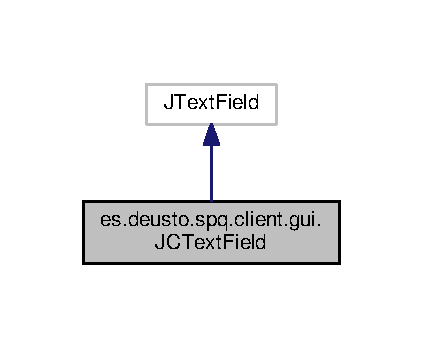
\includegraphics[width=203pt]{classes_1_1deusto_1_1spq_1_1client_1_1gui_1_1_j_c_text_field__inherit__graph}
\end{center}
\end{figure}


Collaboration diagram for es.\+deusto.\+spq.\+client.\+gui.\+J\+C\+Text\+Field\+:\nopagebreak
\begin{figure}[H]
\begin{center}
\leavevmode
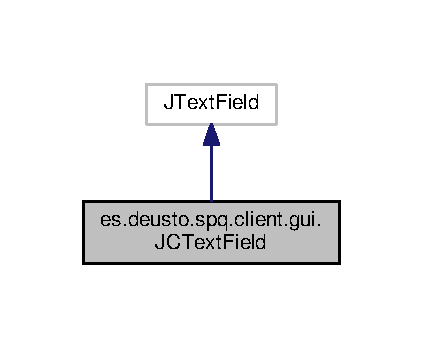
\includegraphics[width=203pt]{classes_1_1deusto_1_1spq_1_1client_1_1gui_1_1_j_c_text_field__coll__graph}
\end{center}
\end{figure}
\subsection*{Public Member Functions}
\begin{DoxyCompactItemize}
\item 
\hyperlink{classes_1_1deusto_1_1spq_1_1client_1_1gui_1_1_j_c_text_field_a389cb6ddbb1e5448d03bc65c8cdb59f1}{J\+C\+Text\+Field} ()
\item 
void \hyperlink{classes_1_1deusto_1_1spq_1_1client_1_1gui_1_1_j_c_text_field_a1bff87e7cb602d355241ac5db6be44f5}{set\+Placeholder} (String placeholder)
\item 
String \hyperlink{classes_1_1deusto_1_1spq_1_1client_1_1gui_1_1_j_c_text_field_a297d538a2d8db4f63a615410d5bac98c}{get\+Placeholder} ()
\item 
Color \hyperlink{classes_1_1deusto_1_1spq_1_1client_1_1gui_1_1_j_c_text_field_a9adf8f2687f87ebadd130282ea7a3a99}{get\+Ph\+Color} ()
\item 
void \hyperlink{classes_1_1deusto_1_1spq_1_1client_1_1gui_1_1_j_c_text_field_ae46eaf9f8f61a4ebb93575624be32e35}{set\+Ph\+Color} (Color ph\+Color)
\item 
void \hyperlink{classes_1_1deusto_1_1spq_1_1client_1_1gui_1_1_j_c_text_field_a71ccd057489e3f8a3264ecee2b4ac8cc}{paint\+Component} (Graphics g)
\end{DoxyCompactItemize}


\subsection{Detailed Description}


Definition at line 12 of file J\+C\+Text\+Field.\+java.



\subsection{Constructor \& Destructor Documentation}
\index{es\+::deusto\+::spq\+::client\+::gui\+::\+J\+C\+Text\+Field@{es\+::deusto\+::spq\+::client\+::gui\+::\+J\+C\+Text\+Field}!J\+C\+Text\+Field@{J\+C\+Text\+Field}}
\index{J\+C\+Text\+Field@{J\+C\+Text\+Field}!es\+::deusto\+::spq\+::client\+::gui\+::\+J\+C\+Text\+Field@{es\+::deusto\+::spq\+::client\+::gui\+::\+J\+C\+Text\+Field}}
\subsubsection[{\texorpdfstring{J\+C\+Text\+Field()}{JCTextField()}}]{\setlength{\rightskip}{0pt plus 5cm}es.\+deusto.\+spq.\+client.\+gui.\+J\+C\+Text\+Field.\+J\+C\+Text\+Field (
\begin{DoxyParamCaption}
{}
\end{DoxyParamCaption}
)}\hypertarget{classes_1_1deusto_1_1spq_1_1client_1_1gui_1_1_j_c_text_field_a389cb6ddbb1e5448d03bc65c8cdb59f1}{}\label{classes_1_1deusto_1_1spq_1_1client_1_1gui_1_1_j_c_text_field_a389cb6ddbb1e5448d03bc65c8cdb59f1}
Constructor de clase 

Definition at line 20 of file J\+C\+Text\+Field.\+java.



\subsection{Member Function Documentation}
\index{es\+::deusto\+::spq\+::client\+::gui\+::\+J\+C\+Text\+Field@{es\+::deusto\+::spq\+::client\+::gui\+::\+J\+C\+Text\+Field}!get\+Ph\+Color@{get\+Ph\+Color}}
\index{get\+Ph\+Color@{get\+Ph\+Color}!es\+::deusto\+::spq\+::client\+::gui\+::\+J\+C\+Text\+Field@{es\+::deusto\+::spq\+::client\+::gui\+::\+J\+C\+Text\+Field}}
\subsubsection[{\texorpdfstring{get\+Ph\+Color()}{getPhColor()}}]{\setlength{\rightskip}{0pt plus 5cm}Color es.\+deusto.\+spq.\+client.\+gui.\+J\+C\+Text\+Field.\+get\+Ph\+Color (
\begin{DoxyParamCaption}
{}
\end{DoxyParamCaption}
)}\hypertarget{classes_1_1deusto_1_1spq_1_1client_1_1gui_1_1_j_c_text_field_a9adf8f2687f87ebadd130282ea7a3a99}{}\label{classes_1_1deusto_1_1spq_1_1client_1_1gui_1_1_j_c_text_field_a9adf8f2687f87ebadd130282ea7a3a99}


Definition at line 58 of file J\+C\+Text\+Field.\+java.

\index{es\+::deusto\+::spq\+::client\+::gui\+::\+J\+C\+Text\+Field@{es\+::deusto\+::spq\+::client\+::gui\+::\+J\+C\+Text\+Field}!get\+Placeholder@{get\+Placeholder}}
\index{get\+Placeholder@{get\+Placeholder}!es\+::deusto\+::spq\+::client\+::gui\+::\+J\+C\+Text\+Field@{es\+::deusto\+::spq\+::client\+::gui\+::\+J\+C\+Text\+Field}}
\subsubsection[{\texorpdfstring{get\+Placeholder()}{getPlaceholder()}}]{\setlength{\rightskip}{0pt plus 5cm}String es.\+deusto.\+spq.\+client.\+gui.\+J\+C\+Text\+Field.\+get\+Placeholder (
\begin{DoxyParamCaption}
{}
\end{DoxyParamCaption}
)}\hypertarget{classes_1_1deusto_1_1spq_1_1client_1_1gui_1_1_j_c_text_field_a297d538a2d8db4f63a615410d5bac98c}{}\label{classes_1_1deusto_1_1spq_1_1client_1_1gui_1_1_j_c_text_field_a297d538a2d8db4f63a615410d5bac98c}


Definition at line 54 of file J\+C\+Text\+Field.\+java.

\index{es\+::deusto\+::spq\+::client\+::gui\+::\+J\+C\+Text\+Field@{es\+::deusto\+::spq\+::client\+::gui\+::\+J\+C\+Text\+Field}!paint\+Component@{paint\+Component}}
\index{paint\+Component@{paint\+Component}!es\+::deusto\+::spq\+::client\+::gui\+::\+J\+C\+Text\+Field@{es\+::deusto\+::spq\+::client\+::gui\+::\+J\+C\+Text\+Field}}
\subsubsection[{\texorpdfstring{paint\+Component(\+Graphics g)}{paintComponent(Graphics g)}}]{\setlength{\rightskip}{0pt plus 5cm}void es.\+deusto.\+spq.\+client.\+gui.\+J\+C\+Text\+Field.\+paint\+Component (
\begin{DoxyParamCaption}
\item[{Graphics}]{g}
\end{DoxyParamCaption}
)}\hypertarget{classes_1_1deusto_1_1spq_1_1client_1_1gui_1_1_j_c_text_field_a71ccd057489e3f8a3264ecee2b4ac8cc}{}\label{classes_1_1deusto_1_1spq_1_1client_1_1gui_1_1_j_c_text_field_a71ccd057489e3f8a3264ecee2b4ac8cc}


Definition at line 67 of file J\+C\+Text\+Field.\+java.

\index{es\+::deusto\+::spq\+::client\+::gui\+::\+J\+C\+Text\+Field@{es\+::deusto\+::spq\+::client\+::gui\+::\+J\+C\+Text\+Field}!set\+Ph\+Color@{set\+Ph\+Color}}
\index{set\+Ph\+Color@{set\+Ph\+Color}!es\+::deusto\+::spq\+::client\+::gui\+::\+J\+C\+Text\+Field@{es\+::deusto\+::spq\+::client\+::gui\+::\+J\+C\+Text\+Field}}
\subsubsection[{\texorpdfstring{set\+Ph\+Color(\+Color ph\+Color)}{setPhColor(Color phColor)}}]{\setlength{\rightskip}{0pt plus 5cm}void es.\+deusto.\+spq.\+client.\+gui.\+J\+C\+Text\+Field.\+set\+Ph\+Color (
\begin{DoxyParamCaption}
\item[{Color}]{ph\+Color}
\end{DoxyParamCaption}
)}\hypertarget{classes_1_1deusto_1_1spq_1_1client_1_1gui_1_1_j_c_text_field_ae46eaf9f8f61a4ebb93575624be32e35}{}\label{classes_1_1deusto_1_1spq_1_1client_1_1gui_1_1_j_c_text_field_ae46eaf9f8f61a4ebb93575624be32e35}


Definition at line 62 of file J\+C\+Text\+Field.\+java.

\index{es\+::deusto\+::spq\+::client\+::gui\+::\+J\+C\+Text\+Field@{es\+::deusto\+::spq\+::client\+::gui\+::\+J\+C\+Text\+Field}!set\+Placeholder@{set\+Placeholder}}
\index{set\+Placeholder@{set\+Placeholder}!es\+::deusto\+::spq\+::client\+::gui\+::\+J\+C\+Text\+Field@{es\+::deusto\+::spq\+::client\+::gui\+::\+J\+C\+Text\+Field}}
\subsubsection[{\texorpdfstring{set\+Placeholder(\+String placeholder)}{setPlaceholder(String placeholder)}}]{\setlength{\rightskip}{0pt plus 5cm}void es.\+deusto.\+spq.\+client.\+gui.\+J\+C\+Text\+Field.\+set\+Placeholder (
\begin{DoxyParamCaption}
\item[{String}]{placeholder}
\end{DoxyParamCaption}
)}\hypertarget{classes_1_1deusto_1_1spq_1_1client_1_1gui_1_1_j_c_text_field_a1bff87e7cb602d355241ac5db6be44f5}{}\label{classes_1_1deusto_1_1spq_1_1client_1_1gui_1_1_j_c_text_field_a1bff87e7cb602d355241ac5db6be44f5}


Definition at line 50 of file J\+C\+Text\+Field.\+java.



Here is the caller graph for this function\+:\nopagebreak
\begin{figure}[H]
\begin{center}
\leavevmode
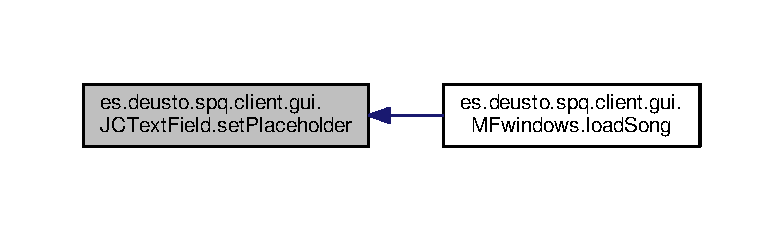
\includegraphics[width=350pt]{classes_1_1deusto_1_1spq_1_1client_1_1gui_1_1_j_c_text_field_a1bff87e7cb602d355241ac5db6be44f5_icgraph}
\end{center}
\end{figure}




The documentation for this class was generated from the following file\+:\begin{DoxyCompactItemize}
\item 
src/main/java/es/deusto/spq/client/gui/\hyperlink{_j_c_text_field_8java}{J\+C\+Text\+Field.\+java}\end{DoxyCompactItemize}

\hypertarget{classes_1_1deusto_1_1spq_1_1server_1_1data_1_1_main}{}\section{es.\+deusto.\+spq.\+server.\+data.\+Main Class Reference}
\label{classes_1_1deusto_1_1spq_1_1server_1_1data_1_1_main}\index{es.\+deusto.\+spq.\+server.\+data.\+Main@{es.\+deusto.\+spq.\+server.\+data.\+Main}}
\subsection*{Static Public Member Functions}
\begin{DoxyCompactItemize}
\item 
static void \hyperlink{classes_1_1deusto_1_1spq_1_1server_1_1data_1_1_main_a54194dc2d03b42c4187475f1bb71ac06}{main} (String args\mbox{[}$\,$\mbox{]})
\end{DoxyCompactItemize}


\subsection{Detailed Description}


Definition at line 6 of file Main.\+java.



\subsection{Member Function Documentation}
\index{es\+::deusto\+::spq\+::server\+::data\+::\+Main@{es\+::deusto\+::spq\+::server\+::data\+::\+Main}!main@{main}}
\index{main@{main}!es\+::deusto\+::spq\+::server\+::data\+::\+Main@{es\+::deusto\+::spq\+::server\+::data\+::\+Main}}
\subsubsection[{\texorpdfstring{main(\+String args[])}{main(String args[])}}]{\setlength{\rightskip}{0pt plus 5cm}static void es.\+deusto.\+spq.\+server.\+data.\+Main.\+main (
\begin{DoxyParamCaption}
\item[{String}]{args\mbox{[}$\,$\mbox{]}}
\end{DoxyParamCaption}
)\hspace{0.3cm}{\ttfamily [static]}}\hypertarget{classes_1_1deusto_1_1spq_1_1server_1_1data_1_1_main_a54194dc2d03b42c4187475f1bb71ac06}{}\label{classes_1_1deusto_1_1spq_1_1server_1_1data_1_1_main_a54194dc2d03b42c4187475f1bb71ac06}


Definition at line 7 of file Main.\+java.



The documentation for this class was generated from the following file\+:\begin{DoxyCompactItemize}
\item 
src/main/java/es/deusto/spq/server/data/\hyperlink{_main_8java}{Main.\+java}\end{DoxyCompactItemize}

\hypertarget{classes_1_1deusto_1_1spq_1_1client_1_1controller_1_1_m_fcontroller}{}\section{es.\+deusto.\+spq.\+client.\+controller.\+M\+Fcontroller Class Reference}
\label{classes_1_1deusto_1_1spq_1_1client_1_1controller_1_1_m_fcontroller}\index{es.\+deusto.\+spq.\+client.\+controller.\+M\+Fcontroller@{es.\+deusto.\+spq.\+client.\+controller.\+M\+Fcontroller}}
\subsection*{Public Member Functions}
\begin{DoxyCompactItemize}
\item 
\hyperlink{classes_1_1deusto_1_1spq_1_1client_1_1controller_1_1_m_fcontroller_ae3acf517cd787cc5db7f40194b50b3a6}{M\+Fcontroller} (String\mbox{[}$\,$\mbox{]} args)  throws Remote\+Exception 
\item 
boolean \hyperlink{classes_1_1deusto_1_1spq_1_1client_1_1controller_1_1_m_fcontroller_a1f86406201f8a172b8aeabc196fd18dc}{register\+User} (String nombre, String apellido, String email, String password)  throws Remote\+Exception 
\item 
boolean \hyperlink{classes_1_1deusto_1_1spq_1_1client_1_1controller_1_1_m_fcontroller_a6f7961fbefdbf44adc004b2e5a7f1568}{login\+User} (String email, String password)  throws Remote\+Exception 
\item 
void \hyperlink{classes_1_1deusto_1_1spq_1_1client_1_1controller_1_1_m_fcontroller_a1085b9339fc5c96ceb989e31d27148f4}{upload\+Song} (String name, String genero, String artista, String cancion, String useridentification)
\item 
boolean \hyperlink{classes_1_1deusto_1_1spq_1_1client_1_1controller_1_1_m_fcontroller_a09cef1dc25fedc61b2b659f3573b6845}{is\+Login} ()
\item 
void \hyperlink{classes_1_1deusto_1_1spq_1_1client_1_1controller_1_1_m_fcontroller_a841cd5e76842d8c50489a3675381e6fb}{set\+Login} (boolean login)
\item 
String \hyperlink{classes_1_1deusto_1_1spq_1_1client_1_1controller_1_1_m_fcontroller_adeab8e80b090fbac2faaf734872d9e0f}{get\+User\+Name} ()  throws Remote\+Exception 
\item 
String \hyperlink{classes_1_1deusto_1_1spq_1_1client_1_1controller_1_1_m_fcontroller_a964e53f75bbb378eb4c10c1e050e92ac}{get\+User\+Identification} ()  throws Remote\+Exception 
\item 
List$<$ String $>$ \hyperlink{classes_1_1deusto_1_1spq_1_1client_1_1controller_1_1_m_fcontroller_a417ee2c4a93e720473db38aaee5a24ba}{load\+Song} ()  throws Remote\+Exception 
\item 
List$<$ String $>$ \hyperlink{classes_1_1deusto_1_1spq_1_1client_1_1controller_1_1_m_fcontroller_a741cf0c10385caaebd3297b3c135b12d}{search\+Song} (String keyword)  throws Remote\+Exception 
\end{DoxyCompactItemize}
\subsection*{Static Public Member Functions}
\begin{DoxyCompactItemize}
\item 
static void \hyperlink{classes_1_1deusto_1_1spq_1_1client_1_1controller_1_1_m_fcontroller_ae5472bcbe3a4f408a94a38cede2c3af9}{main} (String\mbox{[}$\,$\mbox{]} args)  throws Remote\+Exception 
\end{DoxyCompactItemize}


\subsection{Detailed Description}


Definition at line 12 of file M\+Fcontroller.\+java.



\subsection{Constructor \& Destructor Documentation}
\index{es\+::deusto\+::spq\+::client\+::controller\+::\+M\+Fcontroller@{es\+::deusto\+::spq\+::client\+::controller\+::\+M\+Fcontroller}!M\+Fcontroller@{M\+Fcontroller}}
\index{M\+Fcontroller@{M\+Fcontroller}!es\+::deusto\+::spq\+::client\+::controller\+::\+M\+Fcontroller@{es\+::deusto\+::spq\+::client\+::controller\+::\+M\+Fcontroller}}
\subsubsection[{\texorpdfstring{M\+Fcontroller(\+String[] args)}{MFcontroller(String[] args)}}]{\setlength{\rightskip}{0pt plus 5cm}es.\+deusto.\+spq.\+client.\+controller.\+M\+Fcontroller.\+M\+Fcontroller (
\begin{DoxyParamCaption}
\item[{String\mbox{[}$\,$\mbox{]}}]{args}
\end{DoxyParamCaption}
) throws Remote\+Exception}\hypertarget{classes_1_1deusto_1_1spq_1_1client_1_1controller_1_1_m_fcontroller_ae3acf517cd787cc5db7f40194b50b3a6}{}\label{classes_1_1deusto_1_1spq_1_1client_1_1controller_1_1_m_fcontroller_ae3acf517cd787cc5db7f40194b50b3a6}
Constructor de la clase \hyperlink{classes_1_1deusto_1_1spq_1_1client_1_1controller_1_1_m_fcontroller}{M\+Fcontroller}


\begin{DoxyParams}{Parameters}
{\em args} & recibe los argumentos para la configuración de la conexión remota \\
\hline
\end{DoxyParams}

\begin{DoxyExceptions}{Exceptions}
{\em Remote\+Exception} & \\
\hline
\end{DoxyExceptions}


Definition at line 24 of file M\+Fcontroller.\+java.



Here is the call graph for this function\+:\nopagebreak
\begin{figure}[H]
\begin{center}
\leavevmode
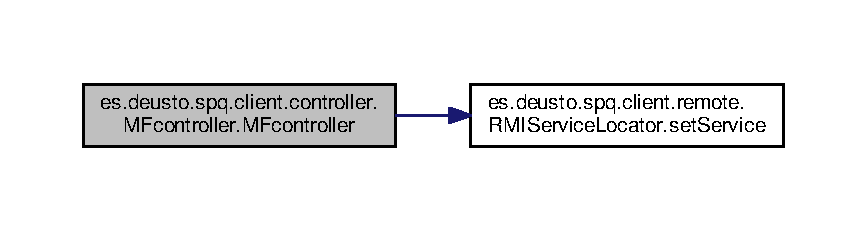
\includegraphics[width=350pt]{classes_1_1deusto_1_1spq_1_1client_1_1controller_1_1_m_fcontroller_ae3acf517cd787cc5db7f40194b50b3a6_cgraph}
\end{center}
\end{figure}




Here is the caller graph for this function\+:\nopagebreak
\begin{figure}[H]
\begin{center}
\leavevmode
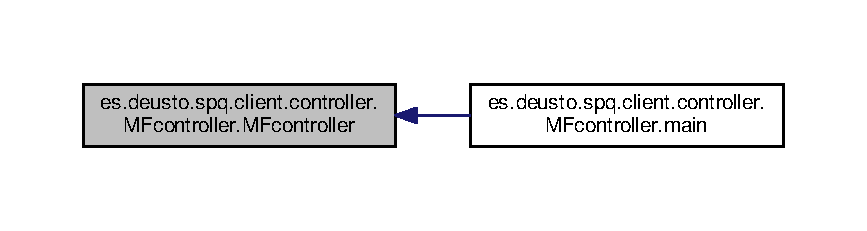
\includegraphics[width=350pt]{classes_1_1deusto_1_1spq_1_1client_1_1controller_1_1_m_fcontroller_ae3acf517cd787cc5db7f40194b50b3a6_icgraph}
\end{center}
\end{figure}




\subsection{Member Function Documentation}
\index{es\+::deusto\+::spq\+::client\+::controller\+::\+M\+Fcontroller@{es\+::deusto\+::spq\+::client\+::controller\+::\+M\+Fcontroller}!get\+User\+Identification@{get\+User\+Identification}}
\index{get\+User\+Identification@{get\+User\+Identification}!es\+::deusto\+::spq\+::client\+::controller\+::\+M\+Fcontroller@{es\+::deusto\+::spq\+::client\+::controller\+::\+M\+Fcontroller}}
\subsubsection[{\texorpdfstring{get\+User\+Identification()}{getUserIdentification()}}]{\setlength{\rightskip}{0pt plus 5cm}String es.\+deusto.\+spq.\+client.\+controller.\+M\+Fcontroller.\+get\+User\+Identification (
\begin{DoxyParamCaption}
{}
\end{DoxyParamCaption}
) throws Remote\+Exception}\hypertarget{classes_1_1deusto_1_1spq_1_1client_1_1controller_1_1_m_fcontroller_a964e53f75bbb378eb4c10c1e050e92ac}{}\label{classes_1_1deusto_1_1spq_1_1client_1_1controller_1_1_m_fcontroller_a964e53f75bbb378eb4c10c1e050e92ac}
The function that return the user identification

\begin{DoxyReturn}{Returns}

\end{DoxyReturn}

\begin{DoxyExceptions}{Exceptions}
{\em Remote\+Exception} & \\
\hline
\end{DoxyExceptions}


Definition at line 123 of file M\+Fcontroller.\+java.



Here is the call graph for this function\+:\nopagebreak
\begin{figure}[H]
\begin{center}
\leavevmode
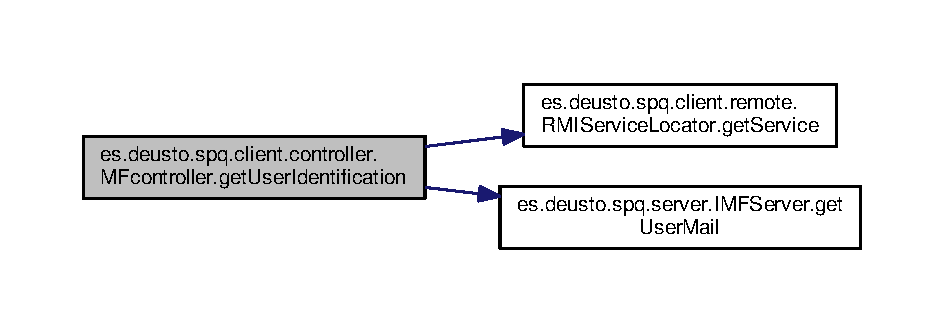
\includegraphics[width=350pt]{classes_1_1deusto_1_1spq_1_1client_1_1controller_1_1_m_fcontroller_a964e53f75bbb378eb4c10c1e050e92ac_cgraph}
\end{center}
\end{figure}




Here is the caller graph for this function\+:\nopagebreak
\begin{figure}[H]
\begin{center}
\leavevmode
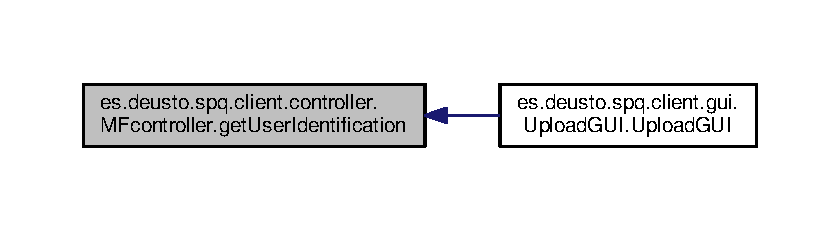
\includegraphics[width=350pt]{classes_1_1deusto_1_1spq_1_1client_1_1controller_1_1_m_fcontroller_a964e53f75bbb378eb4c10c1e050e92ac_icgraph}
\end{center}
\end{figure}


\index{es\+::deusto\+::spq\+::client\+::controller\+::\+M\+Fcontroller@{es\+::deusto\+::spq\+::client\+::controller\+::\+M\+Fcontroller}!get\+User\+Name@{get\+User\+Name}}
\index{get\+User\+Name@{get\+User\+Name}!es\+::deusto\+::spq\+::client\+::controller\+::\+M\+Fcontroller@{es\+::deusto\+::spq\+::client\+::controller\+::\+M\+Fcontroller}}
\subsubsection[{\texorpdfstring{get\+User\+Name()}{getUserName()}}]{\setlength{\rightskip}{0pt plus 5cm}String es.\+deusto.\+spq.\+client.\+controller.\+M\+Fcontroller.\+get\+User\+Name (
\begin{DoxyParamCaption}
{}
\end{DoxyParamCaption}
) throws Remote\+Exception}\hypertarget{classes_1_1deusto_1_1spq_1_1client_1_1controller_1_1_m_fcontroller_adeab8e80b090fbac2faaf734872d9e0f}{}\label{classes_1_1deusto_1_1spq_1_1client_1_1controller_1_1_m_fcontroller_adeab8e80b090fbac2faaf734872d9e0f}
The function that return the user name

\begin{DoxyReturn}{Returns}

\end{DoxyReturn}

\begin{DoxyExceptions}{Exceptions}
{\em Remote\+Exception} & \\
\hline
\end{DoxyExceptions}


Definition at line 113 of file M\+Fcontroller.\+java.



Here is the call graph for this function\+:\nopagebreak
\begin{figure}[H]
\begin{center}
\leavevmode
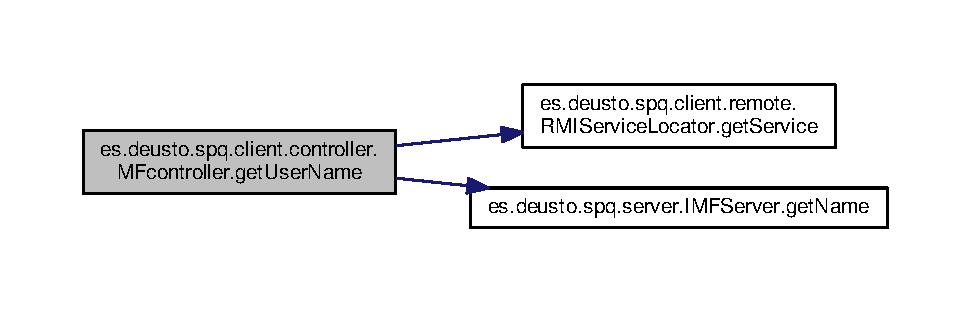
\includegraphics[width=350pt]{classes_1_1deusto_1_1spq_1_1client_1_1controller_1_1_m_fcontroller_adeab8e80b090fbac2faaf734872d9e0f_cgraph}
\end{center}
\end{figure}




Here is the caller graph for this function\+:\nopagebreak
\begin{figure}[H]
\begin{center}
\leavevmode
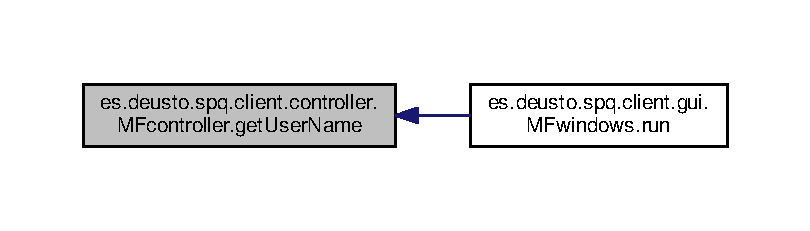
\includegraphics[width=350pt]{classes_1_1deusto_1_1spq_1_1client_1_1controller_1_1_m_fcontroller_adeab8e80b090fbac2faaf734872d9e0f_icgraph}
\end{center}
\end{figure}


\index{es\+::deusto\+::spq\+::client\+::controller\+::\+M\+Fcontroller@{es\+::deusto\+::spq\+::client\+::controller\+::\+M\+Fcontroller}!is\+Login@{is\+Login}}
\index{is\+Login@{is\+Login}!es\+::deusto\+::spq\+::client\+::controller\+::\+M\+Fcontroller@{es\+::deusto\+::spq\+::client\+::controller\+::\+M\+Fcontroller}}
\subsubsection[{\texorpdfstring{is\+Login()}{isLogin()}}]{\setlength{\rightskip}{0pt plus 5cm}boolean es.\+deusto.\+spq.\+client.\+controller.\+M\+Fcontroller.\+is\+Login (
\begin{DoxyParamCaption}
{}
\end{DoxyParamCaption}
)}\hypertarget{classes_1_1deusto_1_1spq_1_1client_1_1controller_1_1_m_fcontroller_a09cef1dc25fedc61b2b659f3573b6845}{}\label{classes_1_1deusto_1_1spq_1_1client_1_1controller_1_1_m_fcontroller_a09cef1dc25fedc61b2b659f3573b6845}
\begin{DoxyReturn}{Returns}
the login 
\end{DoxyReturn}


Definition at line 95 of file M\+Fcontroller.\+java.



Here is the caller graph for this function\+:\nopagebreak
\begin{figure}[H]
\begin{center}
\leavevmode
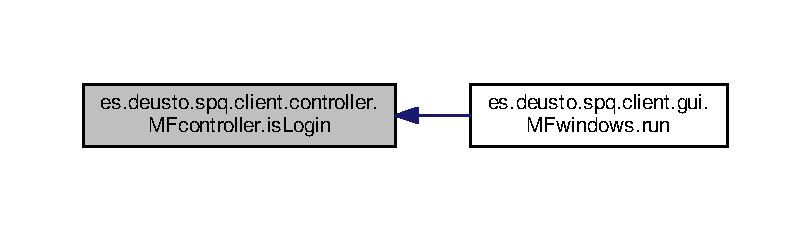
\includegraphics[width=350pt]{classes_1_1deusto_1_1spq_1_1client_1_1controller_1_1_m_fcontroller_a09cef1dc25fedc61b2b659f3573b6845_icgraph}
\end{center}
\end{figure}


\index{es\+::deusto\+::spq\+::client\+::controller\+::\+M\+Fcontroller@{es\+::deusto\+::spq\+::client\+::controller\+::\+M\+Fcontroller}!load\+Song@{load\+Song}}
\index{load\+Song@{load\+Song}!es\+::deusto\+::spq\+::client\+::controller\+::\+M\+Fcontroller@{es\+::deusto\+::spq\+::client\+::controller\+::\+M\+Fcontroller}}
\subsubsection[{\texorpdfstring{load\+Song()}{loadSong()}}]{\setlength{\rightskip}{0pt plus 5cm}List$<$String$>$ es.\+deusto.\+spq.\+client.\+controller.\+M\+Fcontroller.\+load\+Song (
\begin{DoxyParamCaption}
{}
\end{DoxyParamCaption}
) throws Remote\+Exception}\hypertarget{classes_1_1deusto_1_1spq_1_1client_1_1controller_1_1_m_fcontroller_a417ee2c4a93e720473db38aaee5a24ba}{}\label{classes_1_1deusto_1_1spq_1_1client_1_1controller_1_1_m_fcontroller_a417ee2c4a93e720473db38aaee5a24ba}
Load Song method

\begin{DoxyReturn}{Returns}
Return a list of string of songs 
\end{DoxyReturn}

\begin{DoxyExceptions}{Exceptions}
{\em Remote\+Exception} & \\
\hline
\end{DoxyExceptions}


Definition at line 133 of file M\+Fcontroller.\+java.



Here is the call graph for this function\+:\nopagebreak
\begin{figure}[H]
\begin{center}
\leavevmode
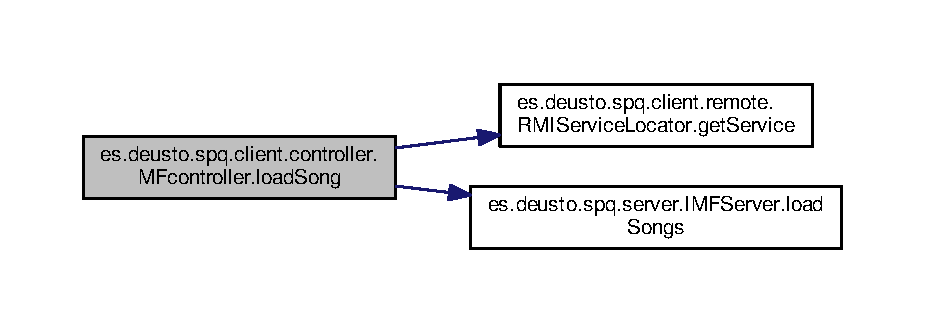
\includegraphics[width=350pt]{classes_1_1deusto_1_1spq_1_1client_1_1controller_1_1_m_fcontroller_a417ee2c4a93e720473db38aaee5a24ba_cgraph}
\end{center}
\end{figure}




Here is the caller graph for this function\+:\nopagebreak
\begin{figure}[H]
\begin{center}
\leavevmode
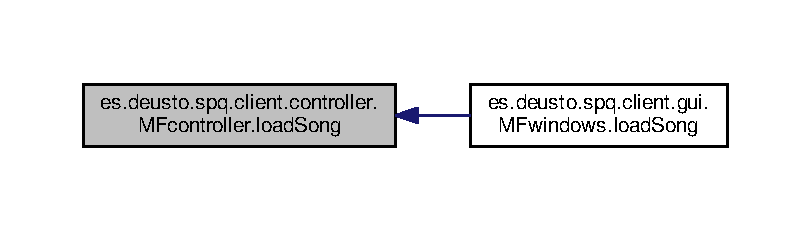
\includegraphics[width=350pt]{classes_1_1deusto_1_1spq_1_1client_1_1controller_1_1_m_fcontroller_a417ee2c4a93e720473db38aaee5a24ba_icgraph}
\end{center}
\end{figure}


\index{es\+::deusto\+::spq\+::client\+::controller\+::\+M\+Fcontroller@{es\+::deusto\+::spq\+::client\+::controller\+::\+M\+Fcontroller}!login\+User@{login\+User}}
\index{login\+User@{login\+User}!es\+::deusto\+::spq\+::client\+::controller\+::\+M\+Fcontroller@{es\+::deusto\+::spq\+::client\+::controller\+::\+M\+Fcontroller}}
\subsubsection[{\texorpdfstring{login\+User(\+String email, String password)}{loginUser(String email, String password)}}]{\setlength{\rightskip}{0pt plus 5cm}boolean es.\+deusto.\+spq.\+client.\+controller.\+M\+Fcontroller.\+login\+User (
\begin{DoxyParamCaption}
\item[{String}]{email, }
\item[{String}]{password}
\end{DoxyParamCaption}
) throws Remote\+Exception}\hypertarget{classes_1_1deusto_1_1spq_1_1client_1_1controller_1_1_m_fcontroller_a6f7961fbefdbf44adc004b2e5a7f1568}{}\label{classes_1_1deusto_1_1spq_1_1client_1_1controller_1_1_m_fcontroller_a6f7961fbefdbf44adc004b2e5a7f1568}
Metoso login que loguea el usuario


\begin{DoxyParams}{Parameters}
{\em email} & el email del usuario \\
\hline
{\em password} & el password del usuario \\
\hline
\end{DoxyParams}
\begin{DoxyReturn}{Returns}
return a boolean true if is logged in successfully 
\end{DoxyReturn}

\begin{DoxyExceptions}{Exceptions}
{\em Remote\+Exception} & \\
\hline
\end{DoxyExceptions}


Definition at line 60 of file M\+Fcontroller.\+java.



Here is the call graph for this function\+:\nopagebreak
\begin{figure}[H]
\begin{center}
\leavevmode
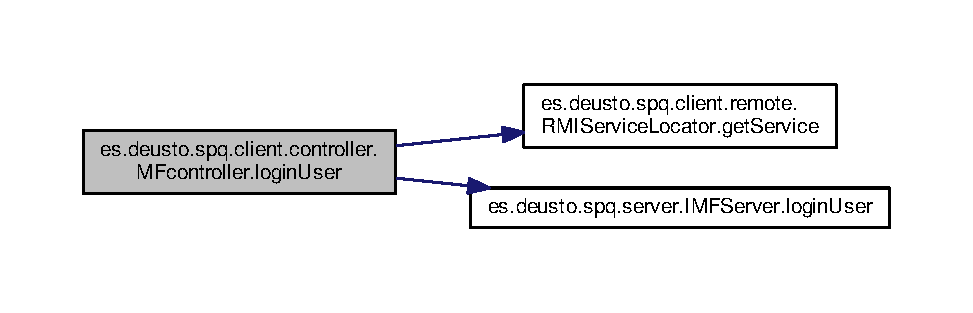
\includegraphics[width=350pt]{classes_1_1deusto_1_1spq_1_1client_1_1controller_1_1_m_fcontroller_a6f7961fbefdbf44adc004b2e5a7f1568_cgraph}
\end{center}
\end{figure}




Here is the caller graph for this function\+:\nopagebreak
\begin{figure}[H]
\begin{center}
\leavevmode
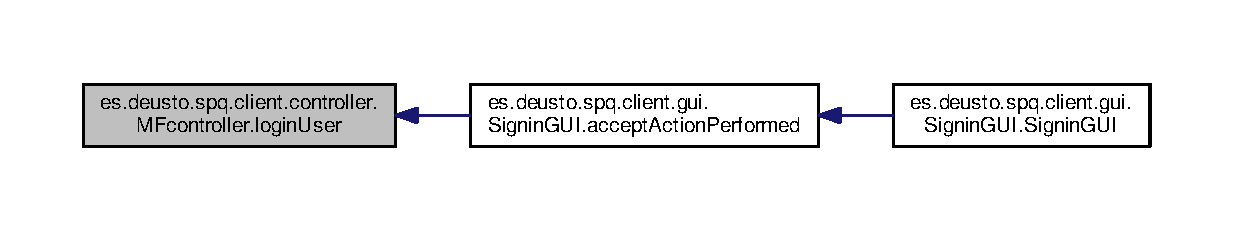
\includegraphics[width=350pt]{classes_1_1deusto_1_1spq_1_1client_1_1controller_1_1_m_fcontroller_a6f7961fbefdbf44adc004b2e5a7f1568_icgraph}
\end{center}
\end{figure}


\index{es\+::deusto\+::spq\+::client\+::controller\+::\+M\+Fcontroller@{es\+::deusto\+::spq\+::client\+::controller\+::\+M\+Fcontroller}!main@{main}}
\index{main@{main}!es\+::deusto\+::spq\+::client\+::controller\+::\+M\+Fcontroller@{es\+::deusto\+::spq\+::client\+::controller\+::\+M\+Fcontroller}}
\subsubsection[{\texorpdfstring{main(\+String[] args)}{main(String[] args)}}]{\setlength{\rightskip}{0pt plus 5cm}static void es.\+deusto.\+spq.\+client.\+controller.\+M\+Fcontroller.\+main (
\begin{DoxyParamCaption}
\item[{String\mbox{[}$\,$\mbox{]}}]{args}
\end{DoxyParamCaption}
) throws Remote\+Exception\hspace{0.3cm}{\ttfamily [static]}}\hypertarget{classes_1_1deusto_1_1spq_1_1client_1_1controller_1_1_m_fcontroller_ae5472bcbe3a4f408a94a38cede2c3af9}{}\label{classes_1_1deusto_1_1spq_1_1client_1_1controller_1_1_m_fcontroller_ae5472bcbe3a4f408a94a38cede2c3af9}
Main method


\begin{DoxyParams}{Parameters}
{\em args} & \\
\hline
\end{DoxyParams}

\begin{DoxyExceptions}{Exceptions}
{\em Remote\+Exception} & \\
\hline
\end{DoxyExceptions}


Definition at line 70 of file M\+Fcontroller.\+java.



Here is the call graph for this function\+:\nopagebreak
\begin{figure}[H]
\begin{center}
\leavevmode
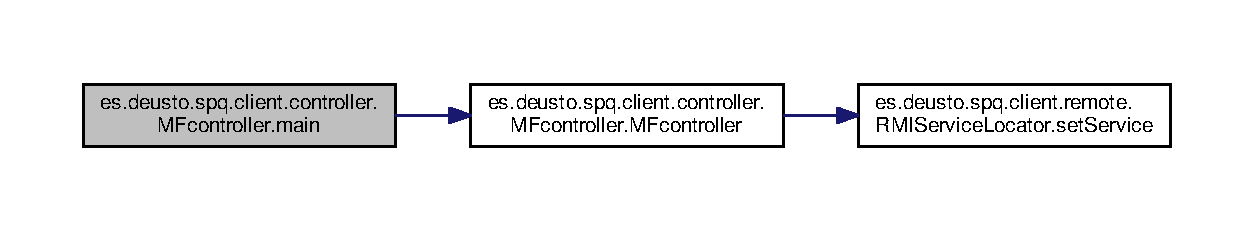
\includegraphics[width=350pt]{classes_1_1deusto_1_1spq_1_1client_1_1controller_1_1_m_fcontroller_ae5472bcbe3a4f408a94a38cede2c3af9_cgraph}
\end{center}
\end{figure}


\index{es\+::deusto\+::spq\+::client\+::controller\+::\+M\+Fcontroller@{es\+::deusto\+::spq\+::client\+::controller\+::\+M\+Fcontroller}!register\+User@{register\+User}}
\index{register\+User@{register\+User}!es\+::deusto\+::spq\+::client\+::controller\+::\+M\+Fcontroller@{es\+::deusto\+::spq\+::client\+::controller\+::\+M\+Fcontroller}}
\subsubsection[{\texorpdfstring{register\+User(\+String nombre, String apellido, String email, String password)}{registerUser(String nombre, String apellido, String email, String password)}}]{\setlength{\rightskip}{0pt plus 5cm}boolean es.\+deusto.\+spq.\+client.\+controller.\+M\+Fcontroller.\+register\+User (
\begin{DoxyParamCaption}
\item[{String}]{nombre, }
\item[{String}]{apellido, }
\item[{String}]{email, }
\item[{String}]{password}
\end{DoxyParamCaption}
) throws Remote\+Exception}\hypertarget{classes_1_1deusto_1_1spq_1_1client_1_1controller_1_1_m_fcontroller_a1f86406201f8a172b8aeabc196fd18dc}{}\label{classes_1_1deusto_1_1spq_1_1client_1_1controller_1_1_m_fcontroller_a1f86406201f8a172b8aeabc196fd18dc}
Metodo que registra el usuario en la bds


\begin{DoxyParams}{Parameters}
{\em nombre} & nombre del usuario \\
\hline
{\em apellido} & apellido del usuario \\
\hline
{\em email} & email del usuario (no puede ser null) \\
\hline
{\em password} & password del usuario (no puede ser null) \\
\hline
\end{DoxyParams}
\begin{DoxyReturn}{Returns}
return a boolean true if is registered successfully 
\end{DoxyReturn}

\begin{DoxyExceptions}{Exceptions}
{\em Remote\+Exception} & \\
\hline
\end{DoxyExceptions}


Definition at line 46 of file M\+Fcontroller.\+java.



Here is the call graph for this function\+:\nopagebreak
\begin{figure}[H]
\begin{center}
\leavevmode
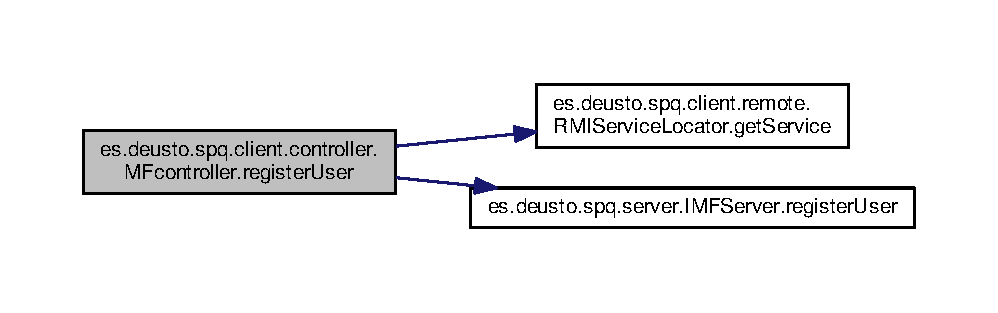
\includegraphics[width=350pt]{classes_1_1deusto_1_1spq_1_1client_1_1controller_1_1_m_fcontroller_a1f86406201f8a172b8aeabc196fd18dc_cgraph}
\end{center}
\end{figure}




Here is the caller graph for this function\+:\nopagebreak
\begin{figure}[H]
\begin{center}
\leavevmode
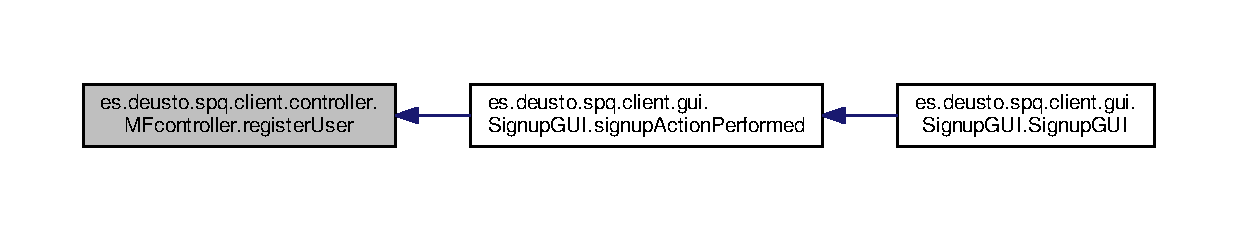
\includegraphics[width=350pt]{classes_1_1deusto_1_1spq_1_1client_1_1controller_1_1_m_fcontroller_a1f86406201f8a172b8aeabc196fd18dc_icgraph}
\end{center}
\end{figure}


\index{es\+::deusto\+::spq\+::client\+::controller\+::\+M\+Fcontroller@{es\+::deusto\+::spq\+::client\+::controller\+::\+M\+Fcontroller}!search\+Song@{search\+Song}}
\index{search\+Song@{search\+Song}!es\+::deusto\+::spq\+::client\+::controller\+::\+M\+Fcontroller@{es\+::deusto\+::spq\+::client\+::controller\+::\+M\+Fcontroller}}
\subsubsection[{\texorpdfstring{search\+Song(\+String keyword)}{searchSong(String keyword)}}]{\setlength{\rightskip}{0pt plus 5cm}List$<$String$>$ es.\+deusto.\+spq.\+client.\+controller.\+M\+Fcontroller.\+search\+Song (
\begin{DoxyParamCaption}
\item[{String}]{keyword}
\end{DoxyParamCaption}
) throws Remote\+Exception}\hypertarget{classes_1_1deusto_1_1spq_1_1client_1_1controller_1_1_m_fcontroller_a741cf0c10385caaebd3297b3c135b12d}{}\label{classes_1_1deusto_1_1spq_1_1client_1_1controller_1_1_m_fcontroller_a741cf0c10385caaebd3297b3c135b12d}
Método de búsqueda de canción se puede buscar por el nombre de la canción, por el artista o por el género de la canción.


\begin{DoxyParams}{Parameters}
{\em keyword} & La palabra clase para la búsqueda \\
\hline
\end{DoxyParams}
\begin{DoxyReturn}{Returns}
Retorna la canción buscado o una lista de canciones 
\end{DoxyReturn}

\begin{DoxyExceptions}{Exceptions}
{\em Remote\+Exception} & \\
\hline
\end{DoxyExceptions}


Definition at line 147 of file M\+Fcontroller.\+java.



Here is the call graph for this function\+:\nopagebreak
\begin{figure}[H]
\begin{center}
\leavevmode
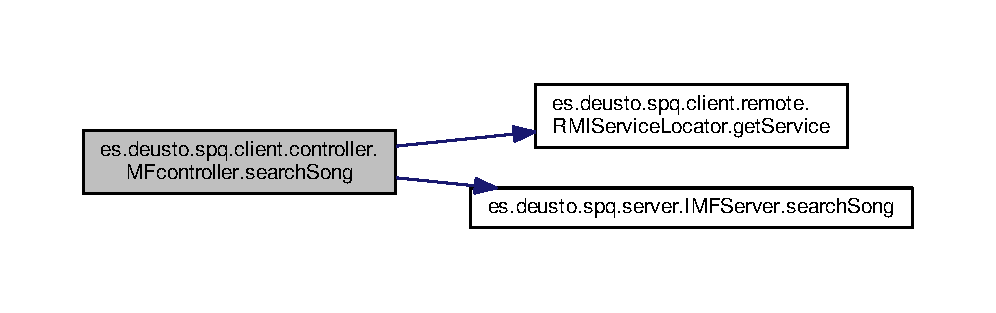
\includegraphics[width=350pt]{classes_1_1deusto_1_1spq_1_1client_1_1controller_1_1_m_fcontroller_a741cf0c10385caaebd3297b3c135b12d_cgraph}
\end{center}
\end{figure}




Here is the caller graph for this function\+:\nopagebreak
\begin{figure}[H]
\begin{center}
\leavevmode
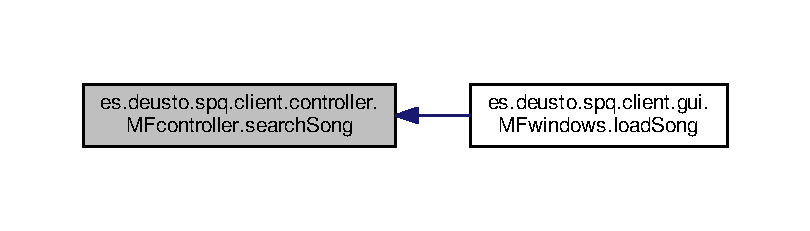
\includegraphics[width=350pt]{classes_1_1deusto_1_1spq_1_1client_1_1controller_1_1_m_fcontroller_a741cf0c10385caaebd3297b3c135b12d_icgraph}
\end{center}
\end{figure}


\index{es\+::deusto\+::spq\+::client\+::controller\+::\+M\+Fcontroller@{es\+::deusto\+::spq\+::client\+::controller\+::\+M\+Fcontroller}!set\+Login@{set\+Login}}
\index{set\+Login@{set\+Login}!es\+::deusto\+::spq\+::client\+::controller\+::\+M\+Fcontroller@{es\+::deusto\+::spq\+::client\+::controller\+::\+M\+Fcontroller}}
\subsubsection[{\texorpdfstring{set\+Login(boolean login)}{setLogin(boolean login)}}]{\setlength{\rightskip}{0pt plus 5cm}void es.\+deusto.\+spq.\+client.\+controller.\+M\+Fcontroller.\+set\+Login (
\begin{DoxyParamCaption}
\item[{boolean}]{login}
\end{DoxyParamCaption}
)}\hypertarget{classes_1_1deusto_1_1spq_1_1client_1_1controller_1_1_m_fcontroller_a841cd5e76842d8c50489a3675381e6fb}{}\label{classes_1_1deusto_1_1spq_1_1client_1_1controller_1_1_m_fcontroller_a841cd5e76842d8c50489a3675381e6fb}

\begin{DoxyParams}{Parameters}
{\em login} & the login to set \\
\hline
\end{DoxyParams}


Definition at line 103 of file M\+Fcontroller.\+java.



Here is the caller graph for this function\+:\nopagebreak
\begin{figure}[H]
\begin{center}
\leavevmode
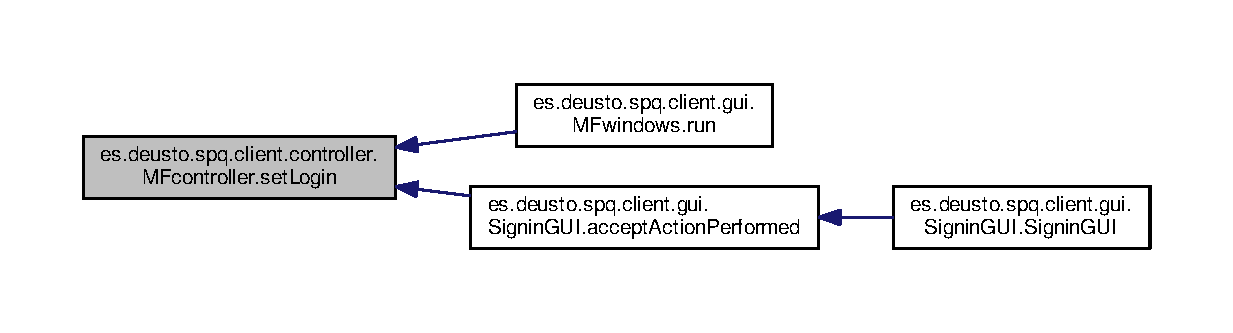
\includegraphics[width=350pt]{classes_1_1deusto_1_1spq_1_1client_1_1controller_1_1_m_fcontroller_a841cd5e76842d8c50489a3675381e6fb_icgraph}
\end{center}
\end{figure}


\index{es\+::deusto\+::spq\+::client\+::controller\+::\+M\+Fcontroller@{es\+::deusto\+::spq\+::client\+::controller\+::\+M\+Fcontroller}!upload\+Song@{upload\+Song}}
\index{upload\+Song@{upload\+Song}!es\+::deusto\+::spq\+::client\+::controller\+::\+M\+Fcontroller@{es\+::deusto\+::spq\+::client\+::controller\+::\+M\+Fcontroller}}
\subsubsection[{\texorpdfstring{upload\+Song(\+String name, String genero, String artista, String cancion, String useridentification)}{uploadSong(String name, String genero, String artista, String cancion, String useridentification)}}]{\setlength{\rightskip}{0pt plus 5cm}void es.\+deusto.\+spq.\+client.\+controller.\+M\+Fcontroller.\+upload\+Song (
\begin{DoxyParamCaption}
\item[{String}]{name, }
\item[{String}]{genero, }
\item[{String}]{artista, }
\item[{String}]{cancion, }
\item[{String}]{useridentification}
\end{DoxyParamCaption}
)}\hypertarget{classes_1_1deusto_1_1spq_1_1client_1_1controller_1_1_m_fcontroller_a1085b9339fc5c96ceb989e31d27148f4}{}\label{classes_1_1deusto_1_1spq_1_1client_1_1controller_1_1_m_fcontroller_a1085b9339fc5c96ceb989e31d27148f4}
Metodo para subir una cancion a la bds


\begin{DoxyParams}{Parameters}
{\em name} & \\
\hline
{\em genero} & \\
\hline
{\em artista} & \\
\hline
{\em cancion} & \\
\hline
{\em useridentification} & \\
\hline
\end{DoxyParams}


Definition at line 83 of file M\+Fcontroller.\+java.



Here is the call graph for this function\+:\nopagebreak
\begin{figure}[H]
\begin{center}
\leavevmode
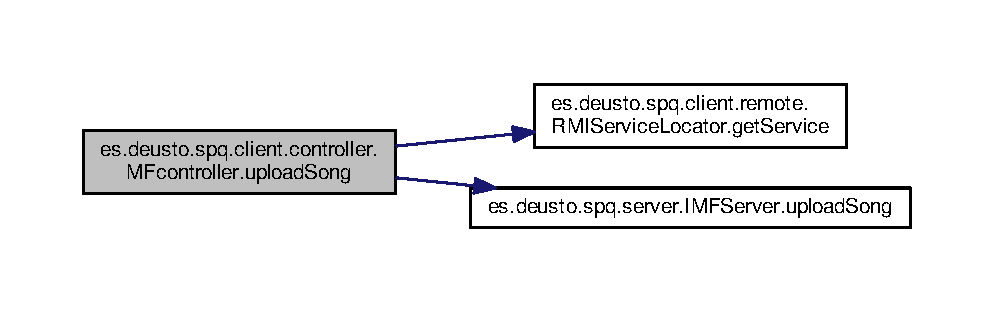
\includegraphics[width=350pt]{classes_1_1deusto_1_1spq_1_1client_1_1controller_1_1_m_fcontroller_a1085b9339fc5c96ceb989e31d27148f4_cgraph}
\end{center}
\end{figure}




Here is the caller graph for this function\+:\nopagebreak
\begin{figure}[H]
\begin{center}
\leavevmode
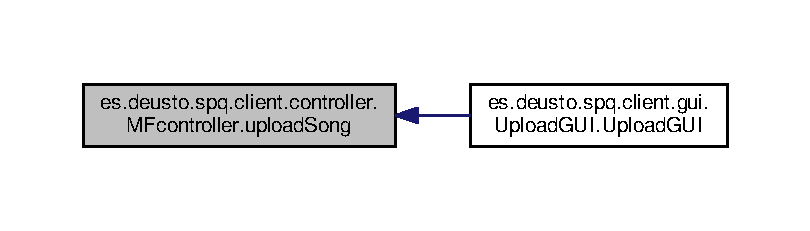
\includegraphics[width=350pt]{classes_1_1deusto_1_1spq_1_1client_1_1controller_1_1_m_fcontroller_a1085b9339fc5c96ceb989e31d27148f4_icgraph}
\end{center}
\end{figure}




The documentation for this class was generated from the following file\+:\begin{DoxyCompactItemize}
\item 
src/main/java/es/deusto/spq/client/controller/\hyperlink{_m_fcontroller_8java}{M\+Fcontroller.\+java}\end{DoxyCompactItemize}

\hypertarget{classes_1_1deusto_1_1spq_1_1server_1_1dao_1_1_m_fdao}{}\section{es.\+deusto.\+spq.\+server.\+dao.\+M\+Fdao Class Reference}
\label{classes_1_1deusto_1_1spq_1_1server_1_1dao_1_1_m_fdao}\index{es.\+deusto.\+spq.\+server.\+dao.\+M\+Fdao@{es.\+deusto.\+spq.\+server.\+dao.\+M\+Fdao}}


Inheritance diagram for es.\+deusto.\+spq.\+server.\+dao.\+M\+Fdao\+:\nopagebreak
\begin{figure}[H]
\begin{center}
\leavevmode
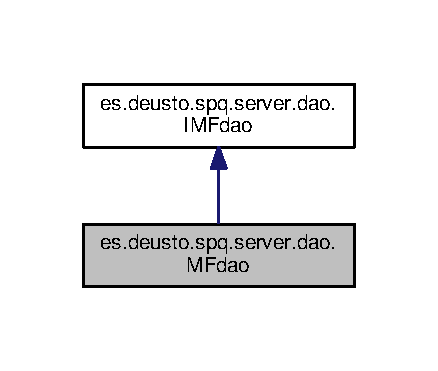
\includegraphics[width=210pt]{classes_1_1deusto_1_1spq_1_1server_1_1dao_1_1_m_fdao__inherit__graph}
\end{center}
\end{figure}


Collaboration diagram for es.\+deusto.\+spq.\+server.\+dao.\+M\+Fdao\+:\nopagebreak
\begin{figure}[H]
\begin{center}
\leavevmode
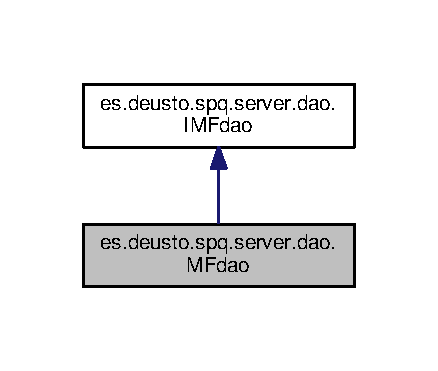
\includegraphics[width=210pt]{classes_1_1deusto_1_1spq_1_1server_1_1dao_1_1_m_fdao__coll__graph}
\end{center}
\end{figure}
\subsection*{Public Member Functions}
\begin{DoxyCompactItemize}
\item 
\hyperlink{classes_1_1deusto_1_1spq_1_1server_1_1dao_1_1_m_fdao_a7395178d95595fd7cc7e3387b435ad73}{M\+Fdao} ()
\item 
boolean \hyperlink{classes_1_1deusto_1_1spq_1_1server_1_1dao_1_1_m_fdao_aa63ea4816fac392840181fb557bf485c}{check\+User} (\hyperlink{classes_1_1deusto_1_1spq_1_1server_1_1data_1_1_usuario}{Usuario} user)
\item 
boolean \hyperlink{classes_1_1deusto_1_1spq_1_1server_1_1dao_1_1_m_fdao_a1444b8fec0c62d8edcccdee255b07457}{login\+User} (String email, String password)
\item 
boolean \hyperlink{classes_1_1deusto_1_1spq_1_1server_1_1dao_1_1_m_fdao_a018654ad3063099187b0005145a36ce6}{store\+User} (\hyperlink{classes_1_1deusto_1_1spq_1_1server_1_1data_1_1_usuario}{Usuario} u)
\item 
String \hyperlink{classes_1_1deusto_1_1spq_1_1server_1_1dao_1_1_m_fdao_af351618006ddba9fcf450f5288808020}{get\+User\+Name} ()
\item 
void \hyperlink{classes_1_1deusto_1_1spq_1_1server_1_1dao_1_1_m_fdao_a4e8d7b5135ed5c9ccb65b6cc499c7278}{store\+Song} (\hyperlink{classes_1_1deusto_1_1spq_1_1server_1_1data_1_1_cancion}{Cancion} c)
\item 
String \hyperlink{classes_1_1deusto_1_1spq_1_1server_1_1dao_1_1_m_fdao_a765a8fa4b291fec932c56c0549adea9a}{get\+User\+Mail} ()
\item 
List$<$ String $>$ \hyperlink{classes_1_1deusto_1_1spq_1_1server_1_1dao_1_1_m_fdao_ab5e0871df69651fdb41d03cdc4cfc25b}{load\+Songs} ()
\item 
List$<$ String $>$ \hyperlink{classes_1_1deusto_1_1spq_1_1server_1_1dao_1_1_m_fdao_a69b3efd8be9b8a2add7d57f703a8f4d7}{search\+Song} (String keyword)
\end{DoxyCompactItemize}


\subsection{Detailed Description}


Definition at line 16 of file M\+Fdao.\+java.



\subsection{Constructor \& Destructor Documentation}
\index{es\+::deusto\+::spq\+::server\+::dao\+::\+M\+Fdao@{es\+::deusto\+::spq\+::server\+::dao\+::\+M\+Fdao}!M\+Fdao@{M\+Fdao}}
\index{M\+Fdao@{M\+Fdao}!es\+::deusto\+::spq\+::server\+::dao\+::\+M\+Fdao@{es\+::deusto\+::spq\+::server\+::dao\+::\+M\+Fdao}}
\subsubsection[{\texorpdfstring{M\+Fdao()}{MFdao()}}]{\setlength{\rightskip}{0pt plus 5cm}es.\+deusto.\+spq.\+server.\+dao.\+M\+Fdao.\+M\+Fdao (
\begin{DoxyParamCaption}
{}
\end{DoxyParamCaption}
)}\hypertarget{classes_1_1deusto_1_1spq_1_1server_1_1dao_1_1_m_fdao_a7395178d95595fd7cc7e3387b435ad73}{}\label{classes_1_1deusto_1_1spq_1_1server_1_1dao_1_1_m_fdao_a7395178d95595fd7cc7e3387b435ad73}
Constructor de mfdao crea un persistence manager factory 

Definition at line 25 of file M\+Fdao.\+java.



\subsection{Member Function Documentation}
\index{es\+::deusto\+::spq\+::server\+::dao\+::\+M\+Fdao@{es\+::deusto\+::spq\+::server\+::dao\+::\+M\+Fdao}!check\+User@{check\+User}}
\index{check\+User@{check\+User}!es\+::deusto\+::spq\+::server\+::dao\+::\+M\+Fdao@{es\+::deusto\+::spq\+::server\+::dao\+::\+M\+Fdao}}
\subsubsection[{\texorpdfstring{check\+User(\+Usuario user)}{checkUser(Usuario user)}}]{\setlength{\rightskip}{0pt plus 5cm}boolean es.\+deusto.\+spq.\+server.\+dao.\+M\+Fdao.\+check\+User (
\begin{DoxyParamCaption}
\item[{{\bf Usuario}}]{user}
\end{DoxyParamCaption}
)}\hypertarget{classes_1_1deusto_1_1spq_1_1server_1_1dao_1_1_m_fdao_aa63ea4816fac392840181fb557bf485c}{}\label{classes_1_1deusto_1_1spq_1_1server_1_1dao_1_1_m_fdao_aa63ea4816fac392840181fb557bf485c}

\begin{DoxyParams}{Parameters}
{\em user} & \\
\hline
\end{DoxyParams}
\begin{DoxyReturn}{Returns}

\end{DoxyReturn}


Implements \hyperlink{interfacees_1_1deusto_1_1spq_1_1server_1_1dao_1_1_i_m_fdao_a2babd39655f8a57f0b64d3bd912e3215}{es.\+deusto.\+spq.\+server.\+dao.\+I\+M\+Fdao}.



Definition at line 58 of file M\+Fdao.\+java.



Here is the call graph for this function\+:\nopagebreak
\begin{figure}[H]
\begin{center}
\leavevmode
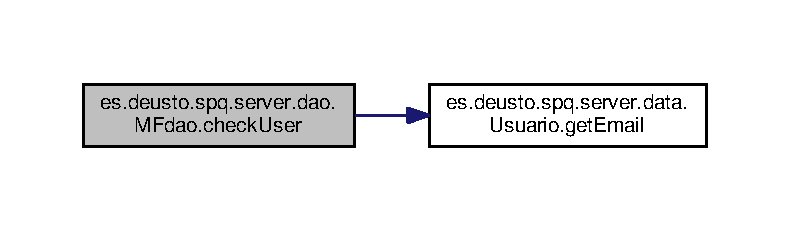
\includegraphics[width=350pt]{classes_1_1deusto_1_1spq_1_1server_1_1dao_1_1_m_fdao_aa63ea4816fac392840181fb557bf485c_cgraph}
\end{center}
\end{figure}




Here is the caller graph for this function\+:\nopagebreak
\begin{figure}[H]
\begin{center}
\leavevmode
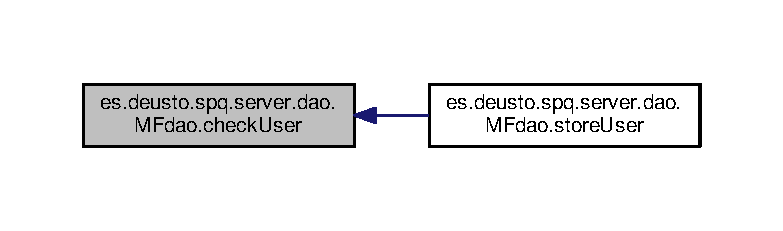
\includegraphics[width=350pt]{classes_1_1deusto_1_1spq_1_1server_1_1dao_1_1_m_fdao_aa63ea4816fac392840181fb557bf485c_icgraph}
\end{center}
\end{figure}


\index{es\+::deusto\+::spq\+::server\+::dao\+::\+M\+Fdao@{es\+::deusto\+::spq\+::server\+::dao\+::\+M\+Fdao}!get\+User\+Mail@{get\+User\+Mail}}
\index{get\+User\+Mail@{get\+User\+Mail}!es\+::deusto\+::spq\+::server\+::dao\+::\+M\+Fdao@{es\+::deusto\+::spq\+::server\+::dao\+::\+M\+Fdao}}
\subsubsection[{\texorpdfstring{get\+User\+Mail()}{getUserMail()}}]{\setlength{\rightskip}{0pt plus 5cm}String es.\+deusto.\+spq.\+server.\+dao.\+M\+Fdao.\+get\+User\+Mail (
\begin{DoxyParamCaption}
{}
\end{DoxyParamCaption}
)}\hypertarget{classes_1_1deusto_1_1spq_1_1server_1_1dao_1_1_m_fdao_a765a8fa4b291fec932c56c0549adea9a}{}\label{classes_1_1deusto_1_1spq_1_1server_1_1dao_1_1_m_fdao_a765a8fa4b291fec932c56c0549adea9a}
\begin{DoxyReturn}{Returns}

\end{DoxyReturn}


Implements \hyperlink{interfacees_1_1deusto_1_1spq_1_1server_1_1dao_1_1_i_m_fdao_acd2152ac1a19753c426b0a0e32dc3e47}{es.\+deusto.\+spq.\+server.\+dao.\+I\+M\+Fdao}.



Definition at line 169 of file M\+Fdao.\+java.

\index{es\+::deusto\+::spq\+::server\+::dao\+::\+M\+Fdao@{es\+::deusto\+::spq\+::server\+::dao\+::\+M\+Fdao}!get\+User\+Name@{get\+User\+Name}}
\index{get\+User\+Name@{get\+User\+Name}!es\+::deusto\+::spq\+::server\+::dao\+::\+M\+Fdao@{es\+::deusto\+::spq\+::server\+::dao\+::\+M\+Fdao}}
\subsubsection[{\texorpdfstring{get\+User\+Name()}{getUserName()}}]{\setlength{\rightskip}{0pt plus 5cm}String es.\+deusto.\+spq.\+server.\+dao.\+M\+Fdao.\+get\+User\+Name (
\begin{DoxyParamCaption}
{}
\end{DoxyParamCaption}
)}\hypertarget{classes_1_1deusto_1_1spq_1_1server_1_1dao_1_1_m_fdao_af351618006ddba9fcf450f5288808020}{}\label{classes_1_1deusto_1_1spq_1_1server_1_1dao_1_1_m_fdao_af351618006ddba9fcf450f5288808020}
\begin{DoxyReturn}{Returns}

\end{DoxyReturn}


Implements \hyperlink{interfacees_1_1deusto_1_1spq_1_1server_1_1dao_1_1_i_m_fdao_a1a090e575d74774692844b5543320fc4}{es.\+deusto.\+spq.\+server.\+dao.\+I\+M\+Fdao}.



Definition at line 129 of file M\+Fdao.\+java.

\index{es\+::deusto\+::spq\+::server\+::dao\+::\+M\+Fdao@{es\+::deusto\+::spq\+::server\+::dao\+::\+M\+Fdao}!load\+Songs@{load\+Songs}}
\index{load\+Songs@{load\+Songs}!es\+::deusto\+::spq\+::server\+::dao\+::\+M\+Fdao@{es\+::deusto\+::spq\+::server\+::dao\+::\+M\+Fdao}}
\subsubsection[{\texorpdfstring{load\+Songs()}{loadSongs()}}]{\setlength{\rightskip}{0pt plus 5cm}List$<$String$>$ es.\+deusto.\+spq.\+server.\+dao.\+M\+Fdao.\+load\+Songs (
\begin{DoxyParamCaption}
{}
\end{DoxyParamCaption}
)}\hypertarget{classes_1_1deusto_1_1spq_1_1server_1_1dao_1_1_m_fdao_ab5e0871df69651fdb41d03cdc4cfc25b}{}\label{classes_1_1deusto_1_1spq_1_1server_1_1dao_1_1_m_fdao_ab5e0871df69651fdb41d03cdc4cfc25b}
\begin{DoxyReturn}{Returns}

\end{DoxyReturn}


Implements \hyperlink{interfacees_1_1deusto_1_1spq_1_1server_1_1dao_1_1_i_m_fdao_a2dbfe3fad8b76ecf116fc3411b3280d5}{es.\+deusto.\+spq.\+server.\+dao.\+I\+M\+Fdao}.



Definition at line 180 of file M\+Fdao.\+java.

\index{es\+::deusto\+::spq\+::server\+::dao\+::\+M\+Fdao@{es\+::deusto\+::spq\+::server\+::dao\+::\+M\+Fdao}!login\+User@{login\+User}}
\index{login\+User@{login\+User}!es\+::deusto\+::spq\+::server\+::dao\+::\+M\+Fdao@{es\+::deusto\+::spq\+::server\+::dao\+::\+M\+Fdao}}
\subsubsection[{\texorpdfstring{login\+User(\+String email, String password)}{loginUser(String email, String password)}}]{\setlength{\rightskip}{0pt plus 5cm}boolean es.\+deusto.\+spq.\+server.\+dao.\+M\+Fdao.\+login\+User (
\begin{DoxyParamCaption}
\item[{String}]{email, }
\item[{String}]{password}
\end{DoxyParamCaption}
)}\hypertarget{classes_1_1deusto_1_1spq_1_1server_1_1dao_1_1_m_fdao_a1444b8fec0c62d8edcccdee255b07457}{}\label{classes_1_1deusto_1_1spq_1_1server_1_1dao_1_1_m_fdao_a1444b8fec0c62d8edcccdee255b07457}

\begin{DoxyParams}{Parameters}
{\em email} & \\
\hline
{\em password} & \\
\hline
\end{DoxyParams}
\begin{DoxyReturn}{Returns}

\end{DoxyReturn}


Implements \hyperlink{interfacees_1_1deusto_1_1spq_1_1server_1_1dao_1_1_i_m_fdao_abc85b827eab8794bd6e00f1df9cf156d}{es.\+deusto.\+spq.\+server.\+dao.\+I\+M\+Fdao}.



Definition at line 85 of file M\+Fdao.\+java.

\index{es\+::deusto\+::spq\+::server\+::dao\+::\+M\+Fdao@{es\+::deusto\+::spq\+::server\+::dao\+::\+M\+Fdao}!search\+Song@{search\+Song}}
\index{search\+Song@{search\+Song}!es\+::deusto\+::spq\+::server\+::dao\+::\+M\+Fdao@{es\+::deusto\+::spq\+::server\+::dao\+::\+M\+Fdao}}
\subsubsection[{\texorpdfstring{search\+Song(\+String keyword)}{searchSong(String keyword)}}]{\setlength{\rightskip}{0pt plus 5cm}List$<$String$>$ es.\+deusto.\+spq.\+server.\+dao.\+M\+Fdao.\+search\+Song (
\begin{DoxyParamCaption}
\item[{String}]{keyword}
\end{DoxyParamCaption}
)}\hypertarget{classes_1_1deusto_1_1spq_1_1server_1_1dao_1_1_m_fdao_a69b3efd8be9b8a2add7d57f703a8f4d7}{}\label{classes_1_1deusto_1_1spq_1_1server_1_1dao_1_1_m_fdao_a69b3efd8be9b8a2add7d57f703a8f4d7}

\begin{DoxyParams}{Parameters}
{\em keyword} & \\
\hline
\end{DoxyParams}
\begin{DoxyReturn}{Returns}

\end{DoxyReturn}


Implements \hyperlink{interfacees_1_1deusto_1_1spq_1_1server_1_1dao_1_1_i_m_fdao_a365443ee24a364f5b4824318ed90af6d}{es.\+deusto.\+spq.\+server.\+dao.\+I\+M\+Fdao}.



Definition at line 213 of file M\+Fdao.\+java.

\index{es\+::deusto\+::spq\+::server\+::dao\+::\+M\+Fdao@{es\+::deusto\+::spq\+::server\+::dao\+::\+M\+Fdao}!store\+Song@{store\+Song}}
\index{store\+Song@{store\+Song}!es\+::deusto\+::spq\+::server\+::dao\+::\+M\+Fdao@{es\+::deusto\+::spq\+::server\+::dao\+::\+M\+Fdao}}
\subsubsection[{\texorpdfstring{store\+Song(\+Cancion c)}{storeSong(Cancion c)}}]{\setlength{\rightskip}{0pt plus 5cm}void es.\+deusto.\+spq.\+server.\+dao.\+M\+Fdao.\+store\+Song (
\begin{DoxyParamCaption}
\item[{{\bf Cancion}}]{c}
\end{DoxyParamCaption}
)}\hypertarget{classes_1_1deusto_1_1spq_1_1server_1_1dao_1_1_m_fdao_a4e8d7b5135ed5c9ccb65b6cc499c7278}{}\label{classes_1_1deusto_1_1spq_1_1server_1_1dao_1_1_m_fdao_a4e8d7b5135ed5c9ccb65b6cc499c7278}

\begin{DoxyParams}{Parameters}
{\em c} & \\
\hline
\end{DoxyParams}


Implements \hyperlink{interfacees_1_1deusto_1_1spq_1_1server_1_1dao_1_1_i_m_fdao_a8d0676aebfd63e2bd07ab7a6ff8e7571}{es.\+deusto.\+spq.\+server.\+dao.\+I\+M\+Fdao}.



Definition at line 140 of file M\+Fdao.\+java.

\index{es\+::deusto\+::spq\+::server\+::dao\+::\+M\+Fdao@{es\+::deusto\+::spq\+::server\+::dao\+::\+M\+Fdao}!store\+User@{store\+User}}
\index{store\+User@{store\+User}!es\+::deusto\+::spq\+::server\+::dao\+::\+M\+Fdao@{es\+::deusto\+::spq\+::server\+::dao\+::\+M\+Fdao}}
\subsubsection[{\texorpdfstring{store\+User(\+Usuario u)}{storeUser(Usuario u)}}]{\setlength{\rightskip}{0pt plus 5cm}boolean es.\+deusto.\+spq.\+server.\+dao.\+M\+Fdao.\+store\+User (
\begin{DoxyParamCaption}
\item[{{\bf Usuario}}]{u}
\end{DoxyParamCaption}
)}\hypertarget{classes_1_1deusto_1_1spq_1_1server_1_1dao_1_1_m_fdao_a018654ad3063099187b0005145a36ce6}{}\label{classes_1_1deusto_1_1spq_1_1server_1_1dao_1_1_m_fdao_a018654ad3063099187b0005145a36ce6}

\begin{DoxyParams}{Parameters}
{\em u} & \\
\hline
\end{DoxyParams}
\begin{DoxyReturn}{Returns}

\end{DoxyReturn}


Implements \hyperlink{interfacees_1_1deusto_1_1spq_1_1server_1_1dao_1_1_i_m_fdao_a3106afd4fe9bbf720f98c8a8c4a9f433}{es.\+deusto.\+spq.\+server.\+dao.\+I\+M\+Fdao}.



Definition at line 113 of file M\+Fdao.\+java.



Here is the call graph for this function\+:\nopagebreak
\begin{figure}[H]
\begin{center}
\leavevmode
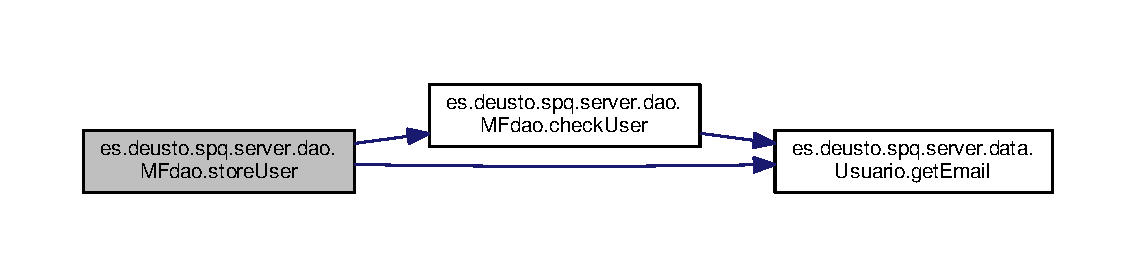
\includegraphics[width=350pt]{classes_1_1deusto_1_1spq_1_1server_1_1dao_1_1_m_fdao_a018654ad3063099187b0005145a36ce6_cgraph}
\end{center}
\end{figure}




The documentation for this class was generated from the following file\+:\begin{DoxyCompactItemize}
\item 
src/main/java/es/deusto/spq/server/dao/\hyperlink{_m_fdao_8java}{M\+Fdao.\+java}\end{DoxyCompactItemize}

\hypertarget{classes_1_1deusto_1_1spq_1_1client_1_1remote_1_1_m_f_manager}{}\section{es.\+deusto.\+spq.\+client.\+remote.\+M\+F\+Manager Class Reference}
\label{classes_1_1deusto_1_1spq_1_1client_1_1remote_1_1_m_f_manager}\index{es.\+deusto.\+spq.\+client.\+remote.\+M\+F\+Manager@{es.\+deusto.\+spq.\+client.\+remote.\+M\+F\+Manager}}
\subsection*{Classes}
\begin{DoxyCompactItemize}
\item 
class {\bfseries java}
\end{DoxyCompactItemize}


\subsection{Detailed Description}


Definition at line 14 of file M\+F\+Manager.\+java.



The documentation for this class was generated from the following file\+:\begin{DoxyCompactItemize}
\item 
src/main/java/es/deusto/spq/client/remote/\hyperlink{_m_f_manager_8java}{M\+F\+Manager.\+java}\end{DoxyCompactItemize}

\hypertarget{classes_1_1deusto_1_1spq_1_1server_1_1_m_f_server}{}\section{es.\+deusto.\+spq.\+server.\+M\+F\+Server Class Reference}
\label{classes_1_1deusto_1_1spq_1_1server_1_1_m_f_server}\index{es.\+deusto.\+spq.\+server.\+M\+F\+Server@{es.\+deusto.\+spq.\+server.\+M\+F\+Server}}


Inheritance diagram for es.\+deusto.\+spq.\+server.\+M\+F\+Server\+:\nopagebreak
\begin{figure}[H]
\begin{center}
\leavevmode
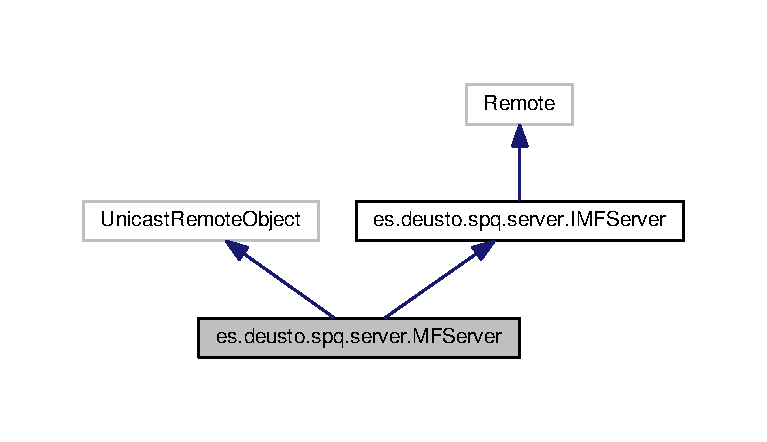
\includegraphics[width=350pt]{classes_1_1deusto_1_1spq_1_1server_1_1_m_f_server__inherit__graph}
\end{center}
\end{figure}


Collaboration diagram for es.\+deusto.\+spq.\+server.\+M\+F\+Server\+:\nopagebreak
\begin{figure}[H]
\begin{center}
\leavevmode
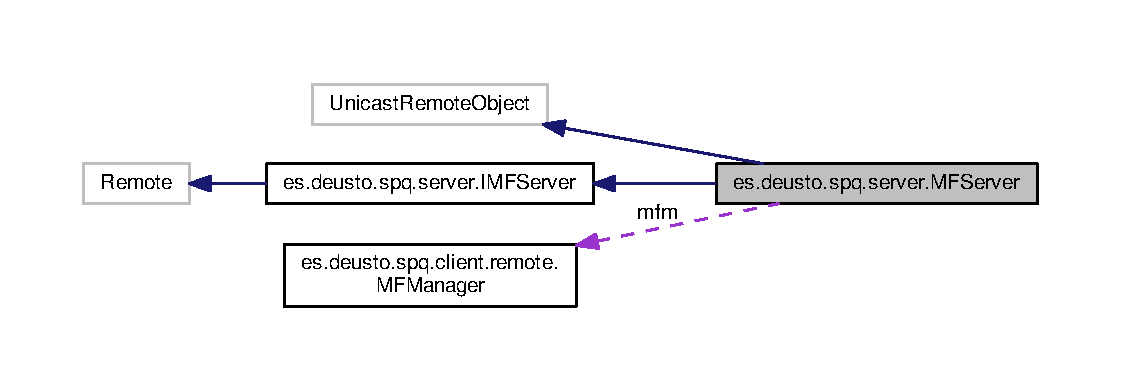
\includegraphics[width=350pt]{classes_1_1deusto_1_1spq_1_1server_1_1_m_f_server__coll__graph}
\end{center}
\end{figure}
\subsection*{Public Member Functions}
\begin{DoxyCompactItemize}
\item 
\hyperlink{classes_1_1deusto_1_1spq_1_1server_1_1_m_f_server_ad42bf68ba9cfc4b560e212df32009cb2}{M\+F\+Server} ()  throws Remote\+Exception 
\item 
boolean \hyperlink{classes_1_1deusto_1_1spq_1_1server_1_1_m_f_server_abf0e32da4f876c11c864593f5d7e39f2}{register\+User} (String nombre, String apellido, String email, String password)  throws Remote\+Exception 
\item 
boolean \hyperlink{classes_1_1deusto_1_1spq_1_1server_1_1_m_f_server_ad242cbf142dbea245a4be10f52b16745}{login\+User} (String email, String password)  throws Remote\+Exception 
\item 
String \hyperlink{classes_1_1deusto_1_1spq_1_1server_1_1_m_f_server_a8d8a50dc58a3b1bd821b95fd30f64af5}{say\+Message} (String login, String password, String message)  throws Remote\+Exception 
\item 
String \hyperlink{classes_1_1deusto_1_1spq_1_1server_1_1_m_f_server_a75eaf5cc57e286889d322248a83a9418}{get\+Name} ()  throws Remote\+Exception 
\item 
void \hyperlink{classes_1_1deusto_1_1spq_1_1server_1_1_m_f_server_a6bd9178166f1294c83144ee792b15cf3}{upload\+Song} (String name, String genero, String artista, String cancion, String useridentification)  throws Remote\+Exception 
\item 
String \hyperlink{classes_1_1deusto_1_1spq_1_1server_1_1_m_f_server_a01d5a6424526e32d8e8ace58776ccad4}{get\+User\+Mail} ()  throws Remote\+Exception 
\item 
List$<$ String $>$ \hyperlink{classes_1_1deusto_1_1spq_1_1server_1_1_m_f_server_ae2c8a121696577c33472b1bad368a1df}{load\+Songs} ()  throws Remote\+Exception 
\item 
List$<$ String $>$ \hyperlink{classes_1_1deusto_1_1spq_1_1server_1_1_m_f_server_ac317c84d14b002d8446046df9345c7ab}{search\+Song} (String keyword)  throws Remote\+Exception 
\end{DoxyCompactItemize}
\subsection*{Static Public Member Functions}
\begin{DoxyCompactItemize}
\item 
static void \hyperlink{classes_1_1deusto_1_1spq_1_1server_1_1_m_f_server_a9cacd13c2c31532f09e0825396a8176d}{main} (String\mbox{[}$\,$\mbox{]} args)
\end{DoxyCompactItemize}


\subsection{Detailed Description}


Definition at line 19 of file M\+F\+Server.\+java.



\subsection{Constructor \& Destructor Documentation}
\index{es\+::deusto\+::spq\+::server\+::\+M\+F\+Server@{es\+::deusto\+::spq\+::server\+::\+M\+F\+Server}!M\+F\+Server@{M\+F\+Server}}
\index{M\+F\+Server@{M\+F\+Server}!es\+::deusto\+::spq\+::server\+::\+M\+F\+Server@{es\+::deusto\+::spq\+::server\+::\+M\+F\+Server}}
\subsubsection[{\texorpdfstring{M\+F\+Server()}{MFServer()}}]{\setlength{\rightskip}{0pt plus 5cm}es.\+deusto.\+spq.\+server.\+M\+F\+Server.\+M\+F\+Server (
\begin{DoxyParamCaption}
{}
\end{DoxyParamCaption}
) throws Remote\+Exception}\hypertarget{classes_1_1deusto_1_1spq_1_1server_1_1_m_f_server_ad42bf68ba9cfc4b560e212df32009cb2}{}\label{classes_1_1deusto_1_1spq_1_1server_1_1_m_f_server_ad42bf68ba9cfc4b560e212df32009cb2}

\begin{DoxyExceptions}{Exceptions}
{\em Remote\+Exception} & \\
\hline
\end{DoxyExceptions}


Definition at line 59 of file M\+F\+Server.\+java.



Here is the caller graph for this function\+:\nopagebreak
\begin{figure}[H]
\begin{center}
\leavevmode
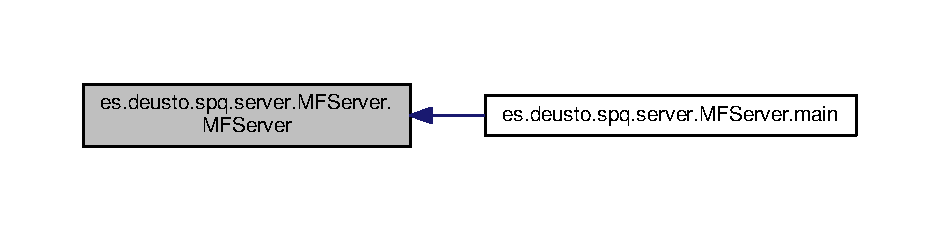
\includegraphics[width=350pt]{classes_1_1deusto_1_1spq_1_1server_1_1_m_f_server_ad42bf68ba9cfc4b560e212df32009cb2_icgraph}
\end{center}
\end{figure}




\subsection{Member Function Documentation}
\index{es\+::deusto\+::spq\+::server\+::\+M\+F\+Server@{es\+::deusto\+::spq\+::server\+::\+M\+F\+Server}!get\+Name@{get\+Name}}
\index{get\+Name@{get\+Name}!es\+::deusto\+::spq\+::server\+::\+M\+F\+Server@{es\+::deusto\+::spq\+::server\+::\+M\+F\+Server}}
\subsubsection[{\texorpdfstring{get\+Name()}{getName()}}]{\setlength{\rightskip}{0pt plus 5cm}String es.\+deusto.\+spq.\+server.\+M\+F\+Server.\+get\+Name (
\begin{DoxyParamCaption}
{}
\end{DoxyParamCaption}
) throws Remote\+Exception}\hypertarget{classes_1_1deusto_1_1spq_1_1server_1_1_m_f_server_a75eaf5cc57e286889d322248a83a9418}{}\label{classes_1_1deusto_1_1spq_1_1server_1_1_m_f_server_a75eaf5cc57e286889d322248a83a9418}


Implements \hyperlink{interfacees_1_1deusto_1_1spq_1_1server_1_1_i_m_f_server_aa5653bb7aa1be80a2d94ebd5785ea409}{es.\+deusto.\+spq.\+server.\+I\+M\+F\+Server}.



Definition at line 106 of file M\+F\+Server.\+java.



Here is the call graph for this function\+:\nopagebreak
\begin{figure}[H]
\begin{center}
\leavevmode
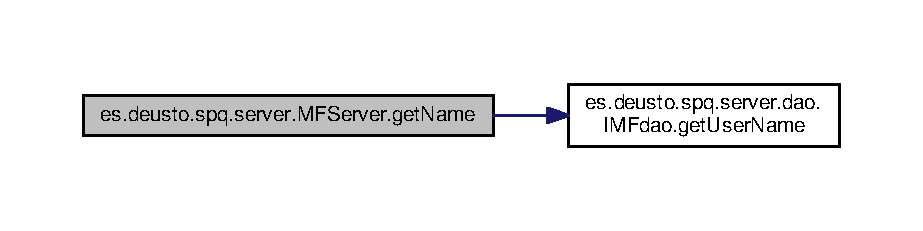
\includegraphics[width=350pt]{classes_1_1deusto_1_1spq_1_1server_1_1_m_f_server_a75eaf5cc57e286889d322248a83a9418_cgraph}
\end{center}
\end{figure}


\index{es\+::deusto\+::spq\+::server\+::\+M\+F\+Server@{es\+::deusto\+::spq\+::server\+::\+M\+F\+Server}!get\+User\+Mail@{get\+User\+Mail}}
\index{get\+User\+Mail@{get\+User\+Mail}!es\+::deusto\+::spq\+::server\+::\+M\+F\+Server@{es\+::deusto\+::spq\+::server\+::\+M\+F\+Server}}
\subsubsection[{\texorpdfstring{get\+User\+Mail()}{getUserMail()}}]{\setlength{\rightskip}{0pt plus 5cm}String es.\+deusto.\+spq.\+server.\+M\+F\+Server.\+get\+User\+Mail (
\begin{DoxyParamCaption}
{}
\end{DoxyParamCaption}
) throws Remote\+Exception}\hypertarget{classes_1_1deusto_1_1spq_1_1server_1_1_m_f_server_a01d5a6424526e32d8e8ace58776ccad4}{}\label{classes_1_1deusto_1_1spq_1_1server_1_1_m_f_server_a01d5a6424526e32d8e8ace58776ccad4}


Implements \hyperlink{interfacees_1_1deusto_1_1spq_1_1server_1_1_i_m_f_server_a009e437ac332036c21d01ceccc217526}{es.\+deusto.\+spq.\+server.\+I\+M\+F\+Server}.



Definition at line 132 of file M\+F\+Server.\+java.



Here is the call graph for this function\+:\nopagebreak
\begin{figure}[H]
\begin{center}
\leavevmode
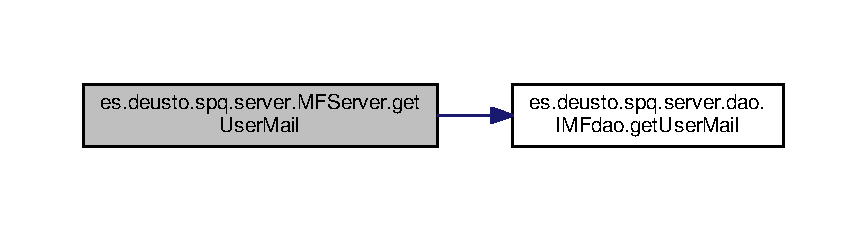
\includegraphics[width=350pt]{classes_1_1deusto_1_1spq_1_1server_1_1_m_f_server_a01d5a6424526e32d8e8ace58776ccad4_cgraph}
\end{center}
\end{figure}


\index{es\+::deusto\+::spq\+::server\+::\+M\+F\+Server@{es\+::deusto\+::spq\+::server\+::\+M\+F\+Server}!load\+Songs@{load\+Songs}}
\index{load\+Songs@{load\+Songs}!es\+::deusto\+::spq\+::server\+::\+M\+F\+Server@{es\+::deusto\+::spq\+::server\+::\+M\+F\+Server}}
\subsubsection[{\texorpdfstring{load\+Songs()}{loadSongs()}}]{\setlength{\rightskip}{0pt plus 5cm}List$<$String$>$ es.\+deusto.\+spq.\+server.\+M\+F\+Server.\+load\+Songs (
\begin{DoxyParamCaption}
{}
\end{DoxyParamCaption}
) throws Remote\+Exception}\hypertarget{classes_1_1deusto_1_1spq_1_1server_1_1_m_f_server_ae2c8a121696577c33472b1bad368a1df}{}\label{classes_1_1deusto_1_1spq_1_1server_1_1_m_f_server_ae2c8a121696577c33472b1bad368a1df}


Implements \hyperlink{interfacees_1_1deusto_1_1spq_1_1server_1_1_i_m_f_server_a3a6e5481a3cc2f543c3ef1e90e4e7da6}{es.\+deusto.\+spq.\+server.\+I\+M\+F\+Server}.



Definition at line 141 of file M\+F\+Server.\+java.



Here is the call graph for this function\+:\nopagebreak
\begin{figure}[H]
\begin{center}
\leavevmode
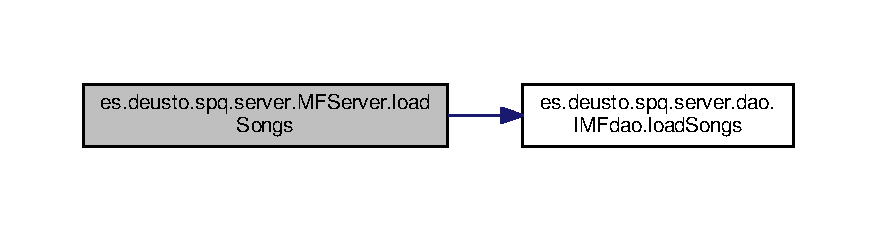
\includegraphics[width=350pt]{classes_1_1deusto_1_1spq_1_1server_1_1_m_f_server_ae2c8a121696577c33472b1bad368a1df_cgraph}
\end{center}
\end{figure}


\index{es\+::deusto\+::spq\+::server\+::\+M\+F\+Server@{es\+::deusto\+::spq\+::server\+::\+M\+F\+Server}!login\+User@{login\+User}}
\index{login\+User@{login\+User}!es\+::deusto\+::spq\+::server\+::\+M\+F\+Server@{es\+::deusto\+::spq\+::server\+::\+M\+F\+Server}}
\subsubsection[{\texorpdfstring{login\+User(\+String email, String password)}{loginUser(String email, String password)}}]{\setlength{\rightskip}{0pt plus 5cm}boolean es.\+deusto.\+spq.\+server.\+M\+F\+Server.\+login\+User (
\begin{DoxyParamCaption}
\item[{String}]{email, }
\item[{String}]{password}
\end{DoxyParamCaption}
) throws Remote\+Exception}\hypertarget{classes_1_1deusto_1_1spq_1_1server_1_1_m_f_server_ad242cbf142dbea245a4be10f52b16745}{}\label{classes_1_1deusto_1_1spq_1_1server_1_1_m_f_server_ad242cbf142dbea245a4be10f52b16745}


Implements \hyperlink{interfacees_1_1deusto_1_1spq_1_1server_1_1_i_m_f_server_afb6983f4de78858b8e73e8f55596374d}{es.\+deusto.\+spq.\+server.\+I\+M\+F\+Server}.



Definition at line 83 of file M\+F\+Server.\+java.



Here is the call graph for this function\+:\nopagebreak
\begin{figure}[H]
\begin{center}
\leavevmode
\includegraphics[width=350pt]{classes_1_1deusto_1_1spq_1_1server_1_1_m_f_server_ad242cbf142dbea245a4be10f52b16745_cgraph}
\end{center}
\end{figure}


\index{es\+::deusto\+::spq\+::server\+::\+M\+F\+Server@{es\+::deusto\+::spq\+::server\+::\+M\+F\+Server}!main@{main}}
\index{main@{main}!es\+::deusto\+::spq\+::server\+::\+M\+F\+Server@{es\+::deusto\+::spq\+::server\+::\+M\+F\+Server}}
\subsubsection[{\texorpdfstring{main(\+String[] args)}{main(String[] args)}}]{\setlength{\rightskip}{0pt plus 5cm}static void es.\+deusto.\+spq.\+server.\+M\+F\+Server.\+main (
\begin{DoxyParamCaption}
\item[{String\mbox{[}$\,$\mbox{]}}]{args}
\end{DoxyParamCaption}
)\hspace{0.3cm}{\ttfamily [static]}}\hypertarget{classes_1_1deusto_1_1spq_1_1server_1_1_m_f_server_a9cacd13c2c31532f09e0825396a8176d}{}\label{classes_1_1deusto_1_1spq_1_1server_1_1_m_f_server_a9cacd13c2c31532f09e0825396a8176d}
The server side main method which establish the remote connexion with the client


\begin{DoxyParams}{Parameters}
{\em args} & \\
\hline
\end{DoxyParams}


Definition at line 30 of file M\+F\+Server.\+java.



Here is the call graph for this function\+:\nopagebreak
\begin{figure}[H]
\begin{center}
\leavevmode
\includegraphics[width=350pt]{classes_1_1deusto_1_1spq_1_1server_1_1_m_f_server_a9cacd13c2c31532f09e0825396a8176d_cgraph}
\end{center}
\end{figure}


\index{es\+::deusto\+::spq\+::server\+::\+M\+F\+Server@{es\+::deusto\+::spq\+::server\+::\+M\+F\+Server}!register\+User@{register\+User}}
\index{register\+User@{register\+User}!es\+::deusto\+::spq\+::server\+::\+M\+F\+Server@{es\+::deusto\+::spq\+::server\+::\+M\+F\+Server}}
\subsubsection[{\texorpdfstring{register\+User(\+String nombre, String apellido, String email, String password)}{registerUser(String nombre, String apellido, String email, String password)}}]{\setlength{\rightskip}{0pt plus 5cm}boolean es.\+deusto.\+spq.\+server.\+M\+F\+Server.\+register\+User (
\begin{DoxyParamCaption}
\item[{String}]{nombre, }
\item[{String}]{apellido, }
\item[{String}]{email, }
\item[{String}]{password}
\end{DoxyParamCaption}
) throws Remote\+Exception}\hypertarget{classes_1_1deusto_1_1spq_1_1server_1_1_m_f_server_abf0e32da4f876c11c864593f5d7e39f2}{}\label{classes_1_1deusto_1_1spq_1_1server_1_1_m_f_server_abf0e32da4f876c11c864593f5d7e39f2}


Implements \hyperlink{interfacees_1_1deusto_1_1spq_1_1server_1_1_i_m_f_server_a51f1f5ea155f4f33ce02d39f7ab9696b}{es.\+deusto.\+spq.\+server.\+I\+M\+F\+Server}.



Definition at line 71 of file M\+F\+Server.\+java.



Here is the call graph for this function\+:\nopagebreak
\begin{figure}[H]
\begin{center}
\leavevmode
\includegraphics[width=350pt]{classes_1_1deusto_1_1spq_1_1server_1_1_m_f_server_abf0e32da4f876c11c864593f5d7e39f2_cgraph}
\end{center}
\end{figure}


\index{es\+::deusto\+::spq\+::server\+::\+M\+F\+Server@{es\+::deusto\+::spq\+::server\+::\+M\+F\+Server}!say\+Message@{say\+Message}}
\index{say\+Message@{say\+Message}!es\+::deusto\+::spq\+::server\+::\+M\+F\+Server@{es\+::deusto\+::spq\+::server\+::\+M\+F\+Server}}
\subsubsection[{\texorpdfstring{say\+Message(\+String login, String password, String message)}{sayMessage(String login, String password, String message)}}]{\setlength{\rightskip}{0pt plus 5cm}String es.\+deusto.\+spq.\+server.\+M\+F\+Server.\+say\+Message (
\begin{DoxyParamCaption}
\item[{String}]{login, }
\item[{String}]{password, }
\item[{String}]{message}
\end{DoxyParamCaption}
) throws Remote\+Exception}\hypertarget{classes_1_1deusto_1_1spq_1_1server_1_1_m_f_server_a8d8a50dc58a3b1bd821b95fd30f64af5}{}\label{classes_1_1deusto_1_1spq_1_1server_1_1_m_f_server_a8d8a50dc58a3b1bd821b95fd30f64af5}


Implements \hyperlink{interfacees_1_1deusto_1_1spq_1_1server_1_1_i_m_f_server_a368aca60ea2ccba7951fc7e3594b7368}{es.\+deusto.\+spq.\+server.\+I\+M\+F\+Server}.



Definition at line 95 of file M\+F\+Server.\+java.

\index{es\+::deusto\+::spq\+::server\+::\+M\+F\+Server@{es\+::deusto\+::spq\+::server\+::\+M\+F\+Server}!search\+Song@{search\+Song}}
\index{search\+Song@{search\+Song}!es\+::deusto\+::spq\+::server\+::\+M\+F\+Server@{es\+::deusto\+::spq\+::server\+::\+M\+F\+Server}}
\subsubsection[{\texorpdfstring{search\+Song(\+String keyword)}{searchSong(String keyword)}}]{\setlength{\rightskip}{0pt plus 5cm}List$<$String$>$ es.\+deusto.\+spq.\+server.\+M\+F\+Server.\+search\+Song (
\begin{DoxyParamCaption}
\item[{String}]{keyword}
\end{DoxyParamCaption}
) throws Remote\+Exception}\hypertarget{classes_1_1deusto_1_1spq_1_1server_1_1_m_f_server_ac317c84d14b002d8446046df9345c7ab}{}\label{classes_1_1deusto_1_1spq_1_1server_1_1_m_f_server_ac317c84d14b002d8446046df9345c7ab}


Implements \hyperlink{interfacees_1_1deusto_1_1spq_1_1server_1_1_i_m_f_server_a4b469cde52367aeb852ff5959ab47bf5}{es.\+deusto.\+spq.\+server.\+I\+M\+F\+Server}.



Definition at line 150 of file M\+F\+Server.\+java.



Here is the call graph for this function\+:\nopagebreak
\begin{figure}[H]
\begin{center}
\leavevmode
\includegraphics[width=350pt]{classes_1_1deusto_1_1spq_1_1server_1_1_m_f_server_ac317c84d14b002d8446046df9345c7ab_cgraph}
\end{center}
\end{figure}


\index{es\+::deusto\+::spq\+::server\+::\+M\+F\+Server@{es\+::deusto\+::spq\+::server\+::\+M\+F\+Server}!upload\+Song@{upload\+Song}}
\index{upload\+Song@{upload\+Song}!es\+::deusto\+::spq\+::server\+::\+M\+F\+Server@{es\+::deusto\+::spq\+::server\+::\+M\+F\+Server}}
\subsubsection[{\texorpdfstring{upload\+Song(\+String name, String genero, String artista, String cancion, String useridentification)}{uploadSong(String name, String genero, String artista, String cancion, String useridentification)}}]{\setlength{\rightskip}{0pt plus 5cm}void es.\+deusto.\+spq.\+server.\+M\+F\+Server.\+upload\+Song (
\begin{DoxyParamCaption}
\item[{String}]{name, }
\item[{String}]{genero, }
\item[{String}]{artista, }
\item[{String}]{cancion, }
\item[{String}]{useridentification}
\end{DoxyParamCaption}
) throws Remote\+Exception}\hypertarget{classes_1_1deusto_1_1spq_1_1server_1_1_m_f_server_a6bd9178166f1294c83144ee792b15cf3}{}\label{classes_1_1deusto_1_1spq_1_1server_1_1_m_f_server_a6bd9178166f1294c83144ee792b15cf3}


Implements \hyperlink{interfacees_1_1deusto_1_1spq_1_1server_1_1_i_m_f_server_ad1c6aec7730ce9a49c61afdc79a9e740}{es.\+deusto.\+spq.\+server.\+I\+M\+F\+Server}.



Definition at line 118 of file M\+F\+Server.\+java.



Here is the call graph for this function\+:\nopagebreak
\begin{figure}[H]
\begin{center}
\leavevmode
\includegraphics[width=350pt]{classes_1_1deusto_1_1spq_1_1server_1_1_m_f_server_a6bd9178166f1294c83144ee792b15cf3_cgraph}
\end{center}
\end{figure}




The documentation for this class was generated from the following file\+:\begin{DoxyCompactItemize}
\item 
src/main/java/es/deusto/spq/server/\hyperlink{_m_f_server_8java}{M\+F\+Server.\+java}\end{DoxyCompactItemize}

\hypertarget{classes_1_1deusto_1_1spq_1_1client_1_1gui_1_1_m_fwindows}{}\section{es.\+deusto.\+spq.\+client.\+gui.\+M\+Fwindows Class Reference}
\label{classes_1_1deusto_1_1spq_1_1client_1_1gui_1_1_m_fwindows}\index{es.\+deusto.\+spq.\+client.\+gui.\+M\+Fwindows@{es.\+deusto.\+spq.\+client.\+gui.\+M\+Fwindows}}


Inheritance diagram for es.\+deusto.\+spq.\+client.\+gui.\+M\+Fwindows\+:\nopagebreak
\begin{figure}[H]
\begin{center}
\leavevmode
\includegraphics[width=207pt]{classes_1_1deusto_1_1spq_1_1client_1_1gui_1_1_m_fwindows__inherit__graph}
\end{center}
\end{figure}


Collaboration diagram for es.\+deusto.\+spq.\+client.\+gui.\+M\+Fwindows\+:\nopagebreak
\begin{figure}[H]
\begin{center}
\leavevmode
\includegraphics[width=350pt]{classes_1_1deusto_1_1spq_1_1client_1_1gui_1_1_m_fwindows__coll__graph}
\end{center}
\end{figure}
\subsection*{Public Member Functions}
\begin{DoxyCompactItemize}
\item 
\hyperlink{classes_1_1deusto_1_1spq_1_1client_1_1gui_1_1_m_fwindows_aaa18b37e7d64acbc168a3357e64f9e32}{M\+Fwindows} (\hyperlink{classes_1_1deusto_1_1spq_1_1client_1_1controller_1_1_m_fcontroller}{M\+Fcontroller} mfcon)  throws Remote\+Exception 
\item 
void \hyperlink{classes_1_1deusto_1_1spq_1_1client_1_1gui_1_1_m_fwindows_a1e95f5476c627804e11ac0b375ff2abc}{centre\+Window} ()
\item 
void \hyperlink{classes_1_1deusto_1_1spq_1_1client_1_1gui_1_1_m_fwindows_af6dc3868f79b8a407d31636a15990e0e}{load\+Song} ()
\item 
void \hyperlink{classes_1_1deusto_1_1spq_1_1client_1_1gui_1_1_m_fwindows_aef184cc4bcdc91fb5e31178af1b46c18}{signin\+Action\+Performed} (Action\+Event e)
\item 
void \hyperlink{classes_1_1deusto_1_1spq_1_1client_1_1gui_1_1_m_fwindows_a2a14396328a4a423871edce84ea58c76}{run} ()
\item 
void \hyperlink{classes_1_1deusto_1_1spq_1_1client_1_1gui_1_1_m_fwindows_a065041d55be69abeb7a179a458e6e8b6}{upload\+Action\+Performed} (Action\+Event e)
\end{DoxyCompactItemize}


\subsection{Detailed Description}
The Free tune application windows class 

Definition at line 17 of file M\+Fwindows.\+java.



\subsection{Constructor \& Destructor Documentation}
\index{es\+::deusto\+::spq\+::client\+::gui\+::\+M\+Fwindows@{es\+::deusto\+::spq\+::client\+::gui\+::\+M\+Fwindows}!M\+Fwindows@{M\+Fwindows}}
\index{M\+Fwindows@{M\+Fwindows}!es\+::deusto\+::spq\+::client\+::gui\+::\+M\+Fwindows@{es\+::deusto\+::spq\+::client\+::gui\+::\+M\+Fwindows}}
\subsubsection[{\texorpdfstring{M\+Fwindows(\+M\+Fcontroller mfcon)}{MFwindows(MFcontroller mfcon)}}]{\setlength{\rightskip}{0pt plus 5cm}es.\+deusto.\+spq.\+client.\+gui.\+M\+Fwindows.\+M\+Fwindows (
\begin{DoxyParamCaption}
\item[{{\bf M\+Fcontroller}}]{mfcon}
\end{DoxyParamCaption}
) throws Remote\+Exception}\hypertarget{classes_1_1deusto_1_1spq_1_1client_1_1gui_1_1_m_fwindows_aaa18b37e7d64acbc168a3357e64f9e32}{}\label{classes_1_1deusto_1_1spq_1_1client_1_1gui_1_1_m_fwindows_aaa18b37e7d64acbc168a3357e64f9e32}
Constructor de la ventana free tune


\begin{DoxyParams}{Parameters}
{\em mfcon} & El controlador de M\+Fcontroller \\
\hline
\end{DoxyParams}

\begin{DoxyExceptions}{Exceptions}
{\em Remote\+Exception} & \\
\hline
\end{DoxyExceptions}


Definition at line 60 of file M\+Fwindows.\+java.



Here is the call graph for this function\+:\nopagebreak
\begin{figure}[H]
\begin{center}
\leavevmode
\includegraphics[width=350pt]{classes_1_1deusto_1_1spq_1_1client_1_1gui_1_1_m_fwindows_aaa18b37e7d64acbc168a3357e64f9e32_cgraph}
\end{center}
\end{figure}




\subsection{Member Function Documentation}
\index{es\+::deusto\+::spq\+::client\+::gui\+::\+M\+Fwindows@{es\+::deusto\+::spq\+::client\+::gui\+::\+M\+Fwindows}!centre\+Window@{centre\+Window}}
\index{centre\+Window@{centre\+Window}!es\+::deusto\+::spq\+::client\+::gui\+::\+M\+Fwindows@{es\+::deusto\+::spq\+::client\+::gui\+::\+M\+Fwindows}}
\subsubsection[{\texorpdfstring{centre\+Window()}{centreWindow()}}]{\setlength{\rightskip}{0pt plus 5cm}void es.\+deusto.\+spq.\+client.\+gui.\+M\+Fwindows.\+centre\+Window (
\begin{DoxyParamCaption}
{}
\end{DoxyParamCaption}
)}\hypertarget{classes_1_1deusto_1_1spq_1_1client_1_1gui_1_1_m_fwindows_a1e95f5476c627804e11ac0b375ff2abc}{}\label{classes_1_1deusto_1_1spq_1_1client_1_1gui_1_1_m_fwindows_a1e95f5476c627804e11ac0b375ff2abc}
Metodo para situar la ventana en el centro 

Definition at line 72 of file M\+Fwindows.\+java.



Here is the caller graph for this function\+:\nopagebreak
\begin{figure}[H]
\begin{center}
\leavevmode
\includegraphics[width=350pt]{classes_1_1deusto_1_1spq_1_1client_1_1gui_1_1_m_fwindows_a1e95f5476c627804e11ac0b375ff2abc_icgraph}
\end{center}
\end{figure}


\index{es\+::deusto\+::spq\+::client\+::gui\+::\+M\+Fwindows@{es\+::deusto\+::spq\+::client\+::gui\+::\+M\+Fwindows}!load\+Song@{load\+Song}}
\index{load\+Song@{load\+Song}!es\+::deusto\+::spq\+::client\+::gui\+::\+M\+Fwindows@{es\+::deusto\+::spq\+::client\+::gui\+::\+M\+Fwindows}}
\subsubsection[{\texorpdfstring{load\+Song()}{loadSong()}}]{\setlength{\rightskip}{0pt plus 5cm}void es.\+deusto.\+spq.\+client.\+gui.\+M\+Fwindows.\+load\+Song (
\begin{DoxyParamCaption}
{}
\end{DoxyParamCaption}
)}\hypertarget{classes_1_1deusto_1_1spq_1_1client_1_1gui_1_1_m_fwindows_af6dc3868f79b8a407d31636a15990e0e}{}\label{classes_1_1deusto_1_1spq_1_1client_1_1gui_1_1_m_fwindows_af6dc3868f79b8a407d31636a15990e0e}


Definition at line 78 of file M\+Fwindows.\+java.



Here is the call graph for this function\+:\nopagebreak
\begin{figure}[H]
\begin{center}
\leavevmode
\includegraphics[width=350pt]{classes_1_1deusto_1_1spq_1_1client_1_1gui_1_1_m_fwindows_af6dc3868f79b8a407d31636a15990e0e_cgraph}
\end{center}
\end{figure}


\index{es\+::deusto\+::spq\+::client\+::gui\+::\+M\+Fwindows@{es\+::deusto\+::spq\+::client\+::gui\+::\+M\+Fwindows}!run@{run}}
\index{run@{run}!es\+::deusto\+::spq\+::client\+::gui\+::\+M\+Fwindows@{es\+::deusto\+::spq\+::client\+::gui\+::\+M\+Fwindows}}
\subsubsection[{\texorpdfstring{run()}{run()}}]{\setlength{\rightskip}{0pt plus 5cm}void es.\+deusto.\+spq.\+client.\+gui.\+M\+Fwindows.\+run (
\begin{DoxyParamCaption}
{}
\end{DoxyParamCaption}
)}\hypertarget{classes_1_1deusto_1_1spq_1_1client_1_1gui_1_1_m_fwindows_a2a14396328a4a423871edce84ea58c76}{}\label{classes_1_1deusto_1_1spq_1_1client_1_1gui_1_1_m_fwindows_a2a14396328a4a423871edce84ea58c76}


Definition at line 295 of file M\+Fwindows.\+java.



Here is the call graph for this function\+:\nopagebreak
\begin{figure}[H]
\begin{center}
\leavevmode
\includegraphics[width=350pt]{classes_1_1deusto_1_1spq_1_1client_1_1gui_1_1_m_fwindows_a2a14396328a4a423871edce84ea58c76_cgraph}
\end{center}
\end{figure}


\index{es\+::deusto\+::spq\+::client\+::gui\+::\+M\+Fwindows@{es\+::deusto\+::spq\+::client\+::gui\+::\+M\+Fwindows}!signin\+Action\+Performed@{signin\+Action\+Performed}}
\index{signin\+Action\+Performed@{signin\+Action\+Performed}!es\+::deusto\+::spq\+::client\+::gui\+::\+M\+Fwindows@{es\+::deusto\+::spq\+::client\+::gui\+::\+M\+Fwindows}}
\subsubsection[{\texorpdfstring{signin\+Action\+Performed(\+Action\+Event e)}{signinActionPerformed(ActionEvent e)}}]{\setlength{\rightskip}{0pt plus 5cm}void es.\+deusto.\+spq.\+client.\+gui.\+M\+Fwindows.\+signin\+Action\+Performed (
\begin{DoxyParamCaption}
\item[{Action\+Event}]{e}
\end{DoxyParamCaption}
)}\hypertarget{classes_1_1deusto_1_1spq_1_1client_1_1gui_1_1_m_fwindows_aef184cc4bcdc91fb5e31178af1b46c18}{}\label{classes_1_1deusto_1_1spq_1_1client_1_1gui_1_1_m_fwindows_aef184cc4bcdc91fb5e31178af1b46c18}
Sign in action performed method


\begin{DoxyParams}{Parameters}
{\em e} & The action event \\
\hline
\end{DoxyParams}


Definition at line 289 of file M\+Fwindows.\+java.



Here is the caller graph for this function\+:\nopagebreak
\begin{figure}[H]
\begin{center}
\leavevmode
\includegraphics[width=350pt]{classes_1_1deusto_1_1spq_1_1client_1_1gui_1_1_m_fwindows_aef184cc4bcdc91fb5e31178af1b46c18_icgraph}
\end{center}
\end{figure}


\index{es\+::deusto\+::spq\+::client\+::gui\+::\+M\+Fwindows@{es\+::deusto\+::spq\+::client\+::gui\+::\+M\+Fwindows}!upload\+Action\+Performed@{upload\+Action\+Performed}}
\index{upload\+Action\+Performed@{upload\+Action\+Performed}!es\+::deusto\+::spq\+::client\+::gui\+::\+M\+Fwindows@{es\+::deusto\+::spq\+::client\+::gui\+::\+M\+Fwindows}}
\subsubsection[{\texorpdfstring{upload\+Action\+Performed(\+Action\+Event e)}{uploadActionPerformed(ActionEvent e)}}]{\setlength{\rightskip}{0pt plus 5cm}void es.\+deusto.\+spq.\+client.\+gui.\+M\+Fwindows.\+upload\+Action\+Performed (
\begin{DoxyParamCaption}
\item[{Action\+Event}]{e}
\end{DoxyParamCaption}
)}\hypertarget{classes_1_1deusto_1_1spq_1_1client_1_1gui_1_1_m_fwindows_a065041d55be69abeb7a179a458e6e8b6}{}\label{classes_1_1deusto_1_1spq_1_1client_1_1gui_1_1_m_fwindows_a065041d55be69abeb7a179a458e6e8b6}


Definition at line 375 of file M\+Fwindows.\+java.



Here is the caller graph for this function\+:\nopagebreak
\begin{figure}[H]
\begin{center}
\leavevmode
\includegraphics[width=350pt]{classes_1_1deusto_1_1spq_1_1client_1_1gui_1_1_m_fwindows_a065041d55be69abeb7a179a458e6e8b6_icgraph}
\end{center}
\end{figure}




The documentation for this class was generated from the following file\+:\begin{DoxyCompactItemize}
\item 
src/main/java/es/deusto/spq/client/gui/\hyperlink{_m_fwindows_8java}{M\+Fwindows.\+java}\end{DoxyCompactItemize}

\hypertarget{classes_1_1deusto_1_1spq_1_1client_1_1gui_1_1_play}{}\section{es.\+deusto.\+spq.\+client.\+gui.\+Play Class Reference}
\label{classes_1_1deusto_1_1spq_1_1client_1_1gui_1_1_play}\index{es.\+deusto.\+spq.\+client.\+gui.\+Play@{es.\+deusto.\+spq.\+client.\+gui.\+Play}}


Inheritance diagram for es.\+deusto.\+spq.\+client.\+gui.\+Play\+:\nopagebreak
\begin{figure}[H]
\begin{center}
\leavevmode
\includegraphics[width=223pt]{classes_1_1deusto_1_1spq_1_1client_1_1gui_1_1_play__inherit__graph}
\end{center}
\end{figure}


Collaboration diagram for es.\+deusto.\+spq.\+client.\+gui.\+Play\+:\nopagebreak
\begin{figure}[H]
\begin{center}
\leavevmode
\includegraphics[width=223pt]{classes_1_1deusto_1_1spq_1_1client_1_1gui_1_1_play__coll__graph}
\end{center}
\end{figure}
\subsection*{Public Member Functions}
\begin{DoxyCompactItemize}
\item 
\hyperlink{classes_1_1deusto_1_1spq_1_1client_1_1gui_1_1_play_a6caae4a347d768940a65a179d767289f}{Play} (String file)
\item 
void \hyperlink{classes_1_1deusto_1_1spq_1_1client_1_1gui_1_1_play_a3f0602abbd8078524b7e10aa11e2be42}{run} ()
\end{DoxyCompactItemize}
\subsection*{Static Public Attributes}
\begin{DoxyCompactItemize}
\item 
static Clip \hyperlink{classes_1_1deusto_1_1spq_1_1client_1_1gui_1_1_play_afbd05e63a18e16480f062c948ba08986}{audio}
\end{DoxyCompactItemize}


\subsection{Detailed Description}


Definition at line 14 of file Play.\+java.



\subsection{Constructor \& Destructor Documentation}
\index{es\+::deusto\+::spq\+::client\+::gui\+::\+Play@{es\+::deusto\+::spq\+::client\+::gui\+::\+Play}!Play@{Play}}
\index{Play@{Play}!es\+::deusto\+::spq\+::client\+::gui\+::\+Play@{es\+::deusto\+::spq\+::client\+::gui\+::\+Play}}
\subsubsection[{\texorpdfstring{Play(\+String file)}{Play(String file)}}]{\setlength{\rightskip}{0pt plus 5cm}es.\+deusto.\+spq.\+client.\+gui.\+Play.\+Play (
\begin{DoxyParamCaption}
\item[{String}]{file}
\end{DoxyParamCaption}
)}\hypertarget{classes_1_1deusto_1_1spq_1_1client_1_1gui_1_1_play_a6caae4a347d768940a65a179d767289f}{}\label{classes_1_1deusto_1_1spq_1_1client_1_1gui_1_1_play_a6caae4a347d768940a65a179d767289f}


Definition at line 19 of file Play.\+java.



\subsection{Member Function Documentation}
\index{es\+::deusto\+::spq\+::client\+::gui\+::\+Play@{es\+::deusto\+::spq\+::client\+::gui\+::\+Play}!run@{run}}
\index{run@{run}!es\+::deusto\+::spq\+::client\+::gui\+::\+Play@{es\+::deusto\+::spq\+::client\+::gui\+::\+Play}}
\subsubsection[{\texorpdfstring{run()}{run()}}]{\setlength{\rightskip}{0pt plus 5cm}void es.\+deusto.\+spq.\+client.\+gui.\+Play.\+run (
\begin{DoxyParamCaption}
{}
\end{DoxyParamCaption}
)}\hypertarget{classes_1_1deusto_1_1spq_1_1client_1_1gui_1_1_play_a3f0602abbd8078524b7e10aa11e2be42}{}\label{classes_1_1deusto_1_1spq_1_1client_1_1gui_1_1_play_a3f0602abbd8078524b7e10aa11e2be42}


Definition at line 25 of file Play.\+java.



\subsection{Member Data Documentation}
\index{es\+::deusto\+::spq\+::client\+::gui\+::\+Play@{es\+::deusto\+::spq\+::client\+::gui\+::\+Play}!audio@{audio}}
\index{audio@{audio}!es\+::deusto\+::spq\+::client\+::gui\+::\+Play@{es\+::deusto\+::spq\+::client\+::gui\+::\+Play}}
\subsubsection[{\texorpdfstring{audio}{audio}}]{\setlength{\rightskip}{0pt plus 5cm}Clip es.\+deusto.\+spq.\+client.\+gui.\+Play.\+audio\hspace{0.3cm}{\ttfamily [static]}}\hypertarget{classes_1_1deusto_1_1spq_1_1client_1_1gui_1_1_play_afbd05e63a18e16480f062c948ba08986}{}\label{classes_1_1deusto_1_1spq_1_1client_1_1gui_1_1_play_afbd05e63a18e16480f062c948ba08986}


Definition at line 17 of file Play.\+java.



The documentation for this class was generated from the following file\+:\begin{DoxyCompactItemize}
\item 
src/main/java/es/deusto/spq/client/gui/\hyperlink{_play_8java}{Play.\+java}\end{DoxyCompactItemize}

\hypertarget{classes_1_1deusto_1_1spq_1_1client_1_1gui_1_1_player}{}\section{es.\+deusto.\+spq.\+client.\+gui.\+Player Class Reference}
\label{classes_1_1deusto_1_1spq_1_1client_1_1gui_1_1_player}\index{es.\+deusto.\+spq.\+client.\+gui.\+Player@{es.\+deusto.\+spq.\+client.\+gui.\+Player}}


Inheritance diagram for es.\+deusto.\+spq.\+client.\+gui.\+Player\+:\nopagebreak
\begin{figure}[H]
\begin{center}
\leavevmode
\includegraphics[width=203pt]{classes_1_1deusto_1_1spq_1_1client_1_1gui_1_1_player__inherit__graph}
\end{center}
\end{figure}


Collaboration diagram for es.\+deusto.\+spq.\+client.\+gui.\+Player\+:\nopagebreak
\begin{figure}[H]
\begin{center}
\leavevmode
\includegraphics[width=234pt]{classes_1_1deusto_1_1spq_1_1client_1_1gui_1_1_player__coll__graph}
\end{center}
\end{figure}
\subsection*{Public Member Functions}
\begin{DoxyCompactItemize}
\item 
\hyperlink{classes_1_1deusto_1_1spq_1_1client_1_1gui_1_1_player_adc29c072a6e982ba28c905346dcd1e44}{Player} (String file)
\item 
void \hyperlink{classes_1_1deusto_1_1spq_1_1client_1_1gui_1_1_player_a86707026d3bfa4bf6cc4ae8221c5ddb8}{run} ()
\item 
Advanced\+Player \hyperlink{classes_1_1deusto_1_1spq_1_1client_1_1gui_1_1_player_a769e39d31eed949195e7f58cab24f095}{get\+Adplay} ()
\item 
void \hyperlink{classes_1_1deusto_1_1spq_1_1client_1_1gui_1_1_player_ac9b34a9a98db187fbed1e9c5afb956f8}{set\+Adplay} (Advanced\+Player adplay)
\end{DoxyCompactItemize}


\subsection{Detailed Description}


Definition at line 9 of file Player.\+java.



\subsection{Constructor \& Destructor Documentation}
\index{es\+::deusto\+::spq\+::client\+::gui\+::\+Player@{es\+::deusto\+::spq\+::client\+::gui\+::\+Player}!Player@{Player}}
\index{Player@{Player}!es\+::deusto\+::spq\+::client\+::gui\+::\+Player@{es\+::deusto\+::spq\+::client\+::gui\+::\+Player}}
\subsubsection[{\texorpdfstring{Player(\+String file)}{Player(String file)}}]{\setlength{\rightskip}{0pt plus 5cm}es.\+deusto.\+spq.\+client.\+gui.\+Player.\+Player (
\begin{DoxyParamCaption}
\item[{String}]{file}
\end{DoxyParamCaption}
)}\hypertarget{classes_1_1deusto_1_1spq_1_1client_1_1gui_1_1_player_adc29c072a6e982ba28c905346dcd1e44}{}\label{classes_1_1deusto_1_1spq_1_1client_1_1gui_1_1_player_adc29c072a6e982ba28c905346dcd1e44}
The player class constructor


\begin{DoxyParams}{Parameters}
{\em file} & \\
\hline
\end{DoxyParams}


Definition at line 18 of file Player.\+java.



\subsection{Member Function Documentation}
\index{es\+::deusto\+::spq\+::client\+::gui\+::\+Player@{es\+::deusto\+::spq\+::client\+::gui\+::\+Player}!get\+Adplay@{get\+Adplay}}
\index{get\+Adplay@{get\+Adplay}!es\+::deusto\+::spq\+::client\+::gui\+::\+Player@{es\+::deusto\+::spq\+::client\+::gui\+::\+Player}}
\subsubsection[{\texorpdfstring{get\+Adplay()}{getAdplay()}}]{\setlength{\rightskip}{0pt plus 5cm}Advanced\+Player es.\+deusto.\+spq.\+client.\+gui.\+Player.\+get\+Adplay (
\begin{DoxyParamCaption}
{}
\end{DoxyParamCaption}
)}\hypertarget{classes_1_1deusto_1_1spq_1_1client_1_1gui_1_1_player_a769e39d31eed949195e7f58cab24f095}{}\label{classes_1_1deusto_1_1spq_1_1client_1_1gui_1_1_player_a769e39d31eed949195e7f58cab24f095}
\begin{DoxyReturn}{Returns}
the adplay 
\end{DoxyReturn}


Definition at line 43 of file Player.\+java.

\index{es\+::deusto\+::spq\+::client\+::gui\+::\+Player@{es\+::deusto\+::spq\+::client\+::gui\+::\+Player}!run@{run}}
\index{run@{run}!es\+::deusto\+::spq\+::client\+::gui\+::\+Player@{es\+::deusto\+::spq\+::client\+::gui\+::\+Player}}
\subsubsection[{\texorpdfstring{run()}{run()}}]{\setlength{\rightskip}{0pt plus 5cm}void es.\+deusto.\+spq.\+client.\+gui.\+Player.\+run (
\begin{DoxyParamCaption}
{}
\end{DoxyParamCaption}
)}\hypertarget{classes_1_1deusto_1_1spq_1_1client_1_1gui_1_1_player_a86707026d3bfa4bf6cc4ae8221c5ddb8}{}\label{classes_1_1deusto_1_1spq_1_1client_1_1gui_1_1_player_a86707026d3bfa4bf6cc4ae8221c5ddb8}


Definition at line 30 of file Player.\+java.

\index{es\+::deusto\+::spq\+::client\+::gui\+::\+Player@{es\+::deusto\+::spq\+::client\+::gui\+::\+Player}!set\+Adplay@{set\+Adplay}}
\index{set\+Adplay@{set\+Adplay}!es\+::deusto\+::spq\+::client\+::gui\+::\+Player@{es\+::deusto\+::spq\+::client\+::gui\+::\+Player}}
\subsubsection[{\texorpdfstring{set\+Adplay(\+Advanced\+Player adplay)}{setAdplay(AdvancedPlayer adplay)}}]{\setlength{\rightskip}{0pt plus 5cm}void es.\+deusto.\+spq.\+client.\+gui.\+Player.\+set\+Adplay (
\begin{DoxyParamCaption}
\item[{Advanced\+Player}]{adplay}
\end{DoxyParamCaption}
)}\hypertarget{classes_1_1deusto_1_1spq_1_1client_1_1gui_1_1_player_ac9b34a9a98db187fbed1e9c5afb956f8}{}\label{classes_1_1deusto_1_1spq_1_1client_1_1gui_1_1_player_ac9b34a9a98db187fbed1e9c5afb956f8}

\begin{DoxyParams}{Parameters}
{\em adplay} & the adplay to set \\
\hline
\end{DoxyParams}


Definition at line 51 of file Player.\+java.



The documentation for this class was generated from the following file\+:\begin{DoxyCompactItemize}
\item 
src/main/java/es/deusto/spq/client/gui/\hyperlink{_player_8java}{Player.\+java}\end{DoxyCompactItemize}

\hypertarget{classes_1_1deusto_1_1spq_1_1client_1_1remote_1_1_r_m_i_service_locator}{}\section{es.\+deusto.\+spq.\+client.\+remote.\+R\+M\+I\+Service\+Locator Class Reference}
\label{classes_1_1deusto_1_1spq_1_1client_1_1remote_1_1_r_m_i_service_locator}\index{es.\+deusto.\+spq.\+client.\+remote.\+R\+M\+I\+Service\+Locator@{es.\+deusto.\+spq.\+client.\+remote.\+R\+M\+I\+Service\+Locator}}
\subsection*{Public Member Functions}
\begin{DoxyCompactItemize}
\item 
\hyperlink{classes_1_1deusto_1_1spq_1_1client_1_1remote_1_1_r_m_i_service_locator_a642cadb2df18622ca837f541c69213dc}{R\+M\+I\+Service\+Locator} ()
\item 
\hyperlink{interfacees_1_1deusto_1_1spq_1_1server_1_1_i_m_f_server}{I\+M\+F\+Server} \hyperlink{classes_1_1deusto_1_1spq_1_1client_1_1remote_1_1_r_m_i_service_locator_a5994c5077ae236bee7323469a89beebb}{get\+Service} ()
\item 
void \hyperlink{classes_1_1deusto_1_1spq_1_1client_1_1remote_1_1_r_m_i_service_locator_a2625caab4b56417ab4215c5da02e500e}{set\+Service} (String ip, String port, String service\+Name)
\end{DoxyCompactItemize}


\subsection{Detailed Description}


Definition at line 11 of file R\+M\+I\+Service\+Locator.\+java.



\subsection{Constructor \& Destructor Documentation}
\index{es\+::deusto\+::spq\+::client\+::remote\+::\+R\+M\+I\+Service\+Locator@{es\+::deusto\+::spq\+::client\+::remote\+::\+R\+M\+I\+Service\+Locator}!R\+M\+I\+Service\+Locator@{R\+M\+I\+Service\+Locator}}
\index{R\+M\+I\+Service\+Locator@{R\+M\+I\+Service\+Locator}!es\+::deusto\+::spq\+::client\+::remote\+::\+R\+M\+I\+Service\+Locator@{es\+::deusto\+::spq\+::client\+::remote\+::\+R\+M\+I\+Service\+Locator}}
\subsubsection[{\texorpdfstring{R\+M\+I\+Service\+Locator()}{RMIServiceLocator()}}]{\setlength{\rightskip}{0pt plus 5cm}es.\+deusto.\+spq.\+client.\+remote.\+R\+M\+I\+Service\+Locator.\+R\+M\+I\+Service\+Locator (
\begin{DoxyParamCaption}
{}
\end{DoxyParamCaption}
)}\hypertarget{classes_1_1deusto_1_1spq_1_1client_1_1remote_1_1_r_m_i_service_locator_a642cadb2df18622ca837f541c69213dc}{}\label{classes_1_1deusto_1_1spq_1_1client_1_1remote_1_1_r_m_i_service_locator_a642cadb2df18622ca837f541c69213dc}


Definition at line 15 of file R\+M\+I\+Service\+Locator.\+java.



\subsection{Member Function Documentation}
\index{es\+::deusto\+::spq\+::client\+::remote\+::\+R\+M\+I\+Service\+Locator@{es\+::deusto\+::spq\+::client\+::remote\+::\+R\+M\+I\+Service\+Locator}!get\+Service@{get\+Service}}
\index{get\+Service@{get\+Service}!es\+::deusto\+::spq\+::client\+::remote\+::\+R\+M\+I\+Service\+Locator@{es\+::deusto\+::spq\+::client\+::remote\+::\+R\+M\+I\+Service\+Locator}}
\subsubsection[{\texorpdfstring{get\+Service()}{getService()}}]{\setlength{\rightskip}{0pt plus 5cm}{\bf I\+M\+F\+Server} es.\+deusto.\+spq.\+client.\+remote.\+R\+M\+I\+Service\+Locator.\+get\+Service (
\begin{DoxyParamCaption}
{}
\end{DoxyParamCaption}
)}\hypertarget{classes_1_1deusto_1_1spq_1_1client_1_1remote_1_1_r_m_i_service_locator_a5994c5077ae236bee7323469a89beebb}{}\label{classes_1_1deusto_1_1spq_1_1client_1_1remote_1_1_r_m_i_service_locator_a5994c5077ae236bee7323469a89beebb}


Definition at line 19 of file R\+M\+I\+Service\+Locator.\+java.



Here is the caller graph for this function\+:\nopagebreak
\begin{figure}[H]
\begin{center}
\leavevmode
\includegraphics[width=350pt]{classes_1_1deusto_1_1spq_1_1client_1_1remote_1_1_r_m_i_service_locator_a5994c5077ae236bee7323469a89beebb_icgraph}
\end{center}
\end{figure}


\index{es\+::deusto\+::spq\+::client\+::remote\+::\+R\+M\+I\+Service\+Locator@{es\+::deusto\+::spq\+::client\+::remote\+::\+R\+M\+I\+Service\+Locator}!set\+Service@{set\+Service}}
\index{set\+Service@{set\+Service}!es\+::deusto\+::spq\+::client\+::remote\+::\+R\+M\+I\+Service\+Locator@{es\+::deusto\+::spq\+::client\+::remote\+::\+R\+M\+I\+Service\+Locator}}
\subsubsection[{\texorpdfstring{set\+Service(\+String ip, String port, String service\+Name)}{setService(String ip, String port, String serviceName)}}]{\setlength{\rightskip}{0pt plus 5cm}void es.\+deusto.\+spq.\+client.\+remote.\+R\+M\+I\+Service\+Locator.\+set\+Service (
\begin{DoxyParamCaption}
\item[{String}]{ip, }
\item[{String}]{port, }
\item[{String}]{service\+Name}
\end{DoxyParamCaption}
)}\hypertarget{classes_1_1deusto_1_1spq_1_1client_1_1remote_1_1_r_m_i_service_locator_a2625caab4b56417ab4215c5da02e500e}{}\label{classes_1_1deusto_1_1spq_1_1client_1_1remote_1_1_r_m_i_service_locator_a2625caab4b56417ab4215c5da02e500e}


Definition at line 23 of file R\+M\+I\+Service\+Locator.\+java.



Here is the caller graph for this function\+:\nopagebreak
\begin{figure}[H]
\begin{center}
\leavevmode
\includegraphics[width=350pt]{classes_1_1deusto_1_1spq_1_1client_1_1remote_1_1_r_m_i_service_locator_a2625caab4b56417ab4215c5da02e500e_icgraph}
\end{center}
\end{figure}




The documentation for this class was generated from the following file\+:\begin{DoxyCompactItemize}
\item 
src/main/java/es/deusto/spq/client/remote/\hyperlink{_r_m_i_service_locator_8java}{R\+M\+I\+Service\+Locator.\+java}\end{DoxyCompactItemize}

\hypertarget{classes_1_1deusto_1_1spq_1_1client_1_1gui_1_1_signin_g_u_i}{}\section{es.\+deusto.\+spq.\+client.\+gui.\+Signin\+G\+UI Class Reference}
\label{classes_1_1deusto_1_1spq_1_1client_1_1gui_1_1_signin_g_u_i}\index{es.\+deusto.\+spq.\+client.\+gui.\+Signin\+G\+UI@{es.\+deusto.\+spq.\+client.\+gui.\+Signin\+G\+UI}}


Inheritance diagram for es.\+deusto.\+spq.\+client.\+gui.\+Signin\+G\+UI\+:\nopagebreak
\begin{figure}[H]
\begin{center}
\leavevmode
\includegraphics[width=203pt]{classes_1_1deusto_1_1spq_1_1client_1_1gui_1_1_signin_g_u_i__inherit__graph}
\end{center}
\end{figure}


Collaboration diagram for es.\+deusto.\+spq.\+client.\+gui.\+Signin\+G\+UI\+:\nopagebreak
\begin{figure}[H]
\begin{center}
\leavevmode
\includegraphics[width=203pt]{classes_1_1deusto_1_1spq_1_1client_1_1gui_1_1_signin_g_u_i__coll__graph}
\end{center}
\end{figure}
\subsection*{Protected Member Functions}
\begin{DoxyCompactItemize}
\item 
\hyperlink{classes_1_1deusto_1_1spq_1_1client_1_1gui_1_1_signin_g_u_i_a24179ffa3dc4cc2e366caa637971a2ed}{Signin\+G\+UI} (\hyperlink{classes_1_1deusto_1_1spq_1_1client_1_1controller_1_1_m_fcontroller}{M\+Fcontroller} mfcon)
\item 
boolean \hyperlink{classes_1_1deusto_1_1spq_1_1client_1_1gui_1_1_signin_g_u_i_af8a81c0d5cf82607229d9ccb32f597fc}{accept\+Action\+Performed} (Action\+Event e)
\end{DoxyCompactItemize}


\subsection{Detailed Description}


Definition at line 25 of file Signin\+G\+U\+I.\+java.



\subsection{Constructor \& Destructor Documentation}
\index{es\+::deusto\+::spq\+::client\+::gui\+::\+Signin\+G\+UI@{es\+::deusto\+::spq\+::client\+::gui\+::\+Signin\+G\+UI}!Signin\+G\+UI@{Signin\+G\+UI}}
\index{Signin\+G\+UI@{Signin\+G\+UI}!es\+::deusto\+::spq\+::client\+::gui\+::\+Signin\+G\+UI@{es\+::deusto\+::spq\+::client\+::gui\+::\+Signin\+G\+UI}}
\subsubsection[{\texorpdfstring{Signin\+G\+U\+I(\+M\+Fcontroller mfcon)}{SigninGUI(MFcontroller mfcon)}}]{\setlength{\rightskip}{0pt plus 5cm}es.\+deusto.\+spq.\+client.\+gui.\+Signin\+G\+U\+I.\+Signin\+G\+UI (
\begin{DoxyParamCaption}
\item[{{\bf M\+Fcontroller}}]{mfcon}
\end{DoxyParamCaption}
)\hspace{0.3cm}{\ttfamily [protected]}}\hypertarget{classes_1_1deusto_1_1spq_1_1client_1_1gui_1_1_signin_g_u_i_a24179ffa3dc4cc2e366caa637971a2ed}{}\label{classes_1_1deusto_1_1spq_1_1client_1_1gui_1_1_signin_g_u_i_a24179ffa3dc4cc2e366caa637971a2ed}
The Signin class constructor 
\begin{DoxyParams}{Parameters}
{\em mfcon} & \\
\hline
\end{DoxyParams}


Definition at line 40 of file Signin\+G\+U\+I.\+java.



Here is the call graph for this function\+:\nopagebreak
\begin{figure}[H]
\begin{center}
\leavevmode
\includegraphics[width=350pt]{classes_1_1deusto_1_1spq_1_1client_1_1gui_1_1_signin_g_u_i_a24179ffa3dc4cc2e366caa637971a2ed_cgraph}
\end{center}
\end{figure}




\subsection{Member Function Documentation}
\index{es\+::deusto\+::spq\+::client\+::gui\+::\+Signin\+G\+UI@{es\+::deusto\+::spq\+::client\+::gui\+::\+Signin\+G\+UI}!accept\+Action\+Performed@{accept\+Action\+Performed}}
\index{accept\+Action\+Performed@{accept\+Action\+Performed}!es\+::deusto\+::spq\+::client\+::gui\+::\+Signin\+G\+UI@{es\+::deusto\+::spq\+::client\+::gui\+::\+Signin\+G\+UI}}
\subsubsection[{\texorpdfstring{accept\+Action\+Performed(\+Action\+Event e)}{acceptActionPerformed(ActionEvent e)}}]{\setlength{\rightskip}{0pt plus 5cm}boolean es.\+deusto.\+spq.\+client.\+gui.\+Signin\+G\+U\+I.\+accept\+Action\+Performed (
\begin{DoxyParamCaption}
\item[{Action\+Event}]{e}
\end{DoxyParamCaption}
)\hspace{0.3cm}{\ttfamily [protected]}}\hypertarget{classes_1_1deusto_1_1spq_1_1client_1_1gui_1_1_signin_g_u_i_af8a81c0d5cf82607229d9ccb32f597fc}{}\label{classes_1_1deusto_1_1spq_1_1client_1_1gui_1_1_signin_g_u_i_af8a81c0d5cf82607229d9ccb32f597fc}


Definition at line 107 of file Signin\+G\+U\+I.\+java.



Here is the call graph for this function\+:\nopagebreak
\begin{figure}[H]
\begin{center}
\leavevmode
\includegraphics[width=350pt]{classes_1_1deusto_1_1spq_1_1client_1_1gui_1_1_signin_g_u_i_af8a81c0d5cf82607229d9ccb32f597fc_cgraph}
\end{center}
\end{figure}




Here is the caller graph for this function\+:\nopagebreak
\begin{figure}[H]
\begin{center}
\leavevmode
\includegraphics[width=350pt]{classes_1_1deusto_1_1spq_1_1client_1_1gui_1_1_signin_g_u_i_af8a81c0d5cf82607229d9ccb32f597fc_icgraph}
\end{center}
\end{figure}




The documentation for this class was generated from the following file\+:\begin{DoxyCompactItemize}
\item 
src/main/java/es/deusto/spq/client/gui/\hyperlink{_signin_g_u_i_8java}{Signin\+G\+U\+I.\+java}\end{DoxyCompactItemize}

\hypertarget{classes_1_1deusto_1_1spq_1_1client_1_1gui_1_1_signup_g_u_i}{}\section{es.\+deusto.\+spq.\+client.\+gui.\+Signup\+G\+UI Class Reference}
\label{classes_1_1deusto_1_1spq_1_1client_1_1gui_1_1_signup_g_u_i}\index{es.\+deusto.\+spq.\+client.\+gui.\+Signup\+G\+UI@{es.\+deusto.\+spq.\+client.\+gui.\+Signup\+G\+UI}}


Inheritance diagram for es.\+deusto.\+spq.\+client.\+gui.\+Signup\+G\+UI\+:\nopagebreak
\begin{figure}[H]
\begin{center}
\leavevmode
\includegraphics[width=203pt]{classes_1_1deusto_1_1spq_1_1client_1_1gui_1_1_signup_g_u_i__inherit__graph}
\end{center}
\end{figure}


Collaboration diagram for es.\+deusto.\+spq.\+client.\+gui.\+Signup\+G\+UI\+:\nopagebreak
\begin{figure}[H]
\begin{center}
\leavevmode
\includegraphics[width=203pt]{classes_1_1deusto_1_1spq_1_1client_1_1gui_1_1_signup_g_u_i__coll__graph}
\end{center}
\end{figure}
\subsection*{Protected Member Functions}
\begin{DoxyCompactItemize}
\item 
\hyperlink{classes_1_1deusto_1_1spq_1_1client_1_1gui_1_1_signup_g_u_i_aa80f61956033cb2a3b8541834d2cc973}{Signup\+G\+UI} (\hyperlink{classes_1_1deusto_1_1spq_1_1client_1_1controller_1_1_m_fcontroller}{M\+Fcontroller} mfcon)
\item 
boolean \hyperlink{classes_1_1deusto_1_1spq_1_1client_1_1gui_1_1_signup_g_u_i_a66051677d5a7b866ae8c32875d84c78b}{signup\+Action\+Performed} (Action\+Event e)
\end{DoxyCompactItemize}


\subsection{Detailed Description}


Definition at line 21 of file Signup\+G\+U\+I.\+java.



\subsection{Constructor \& Destructor Documentation}
\index{es\+::deusto\+::spq\+::client\+::gui\+::\+Signup\+G\+UI@{es\+::deusto\+::spq\+::client\+::gui\+::\+Signup\+G\+UI}!Signup\+G\+UI@{Signup\+G\+UI}}
\index{Signup\+G\+UI@{Signup\+G\+UI}!es\+::deusto\+::spq\+::client\+::gui\+::\+Signup\+G\+UI@{es\+::deusto\+::spq\+::client\+::gui\+::\+Signup\+G\+UI}}
\subsubsection[{\texorpdfstring{Signup\+G\+U\+I(\+M\+Fcontroller mfcon)}{SignupGUI(MFcontroller mfcon)}}]{\setlength{\rightskip}{0pt plus 5cm}es.\+deusto.\+spq.\+client.\+gui.\+Signup\+G\+U\+I.\+Signup\+G\+UI (
\begin{DoxyParamCaption}
\item[{{\bf M\+Fcontroller}}]{mfcon}
\end{DoxyParamCaption}
)\hspace{0.3cm}{\ttfamily [protected]}}\hypertarget{classes_1_1deusto_1_1spq_1_1client_1_1gui_1_1_signup_g_u_i_aa80f61956033cb2a3b8541834d2cc973}{}\label{classes_1_1deusto_1_1spq_1_1client_1_1gui_1_1_signup_g_u_i_aa80f61956033cb2a3b8541834d2cc973}
Create the frame. 

Definition at line 38 of file Signup\+G\+U\+I.\+java.



Here is the call graph for this function\+:\nopagebreak
\begin{figure}[H]
\begin{center}
\leavevmode
\includegraphics[width=350pt]{classes_1_1deusto_1_1spq_1_1client_1_1gui_1_1_signup_g_u_i_aa80f61956033cb2a3b8541834d2cc973_cgraph}
\end{center}
\end{figure}




\subsection{Member Function Documentation}
\index{es\+::deusto\+::spq\+::client\+::gui\+::\+Signup\+G\+UI@{es\+::deusto\+::spq\+::client\+::gui\+::\+Signup\+G\+UI}!signup\+Action\+Performed@{signup\+Action\+Performed}}
\index{signup\+Action\+Performed@{signup\+Action\+Performed}!es\+::deusto\+::spq\+::client\+::gui\+::\+Signup\+G\+UI@{es\+::deusto\+::spq\+::client\+::gui\+::\+Signup\+G\+UI}}
\subsubsection[{\texorpdfstring{signup\+Action\+Performed(\+Action\+Event e)}{signupActionPerformed(ActionEvent e)}}]{\setlength{\rightskip}{0pt plus 5cm}boolean es.\+deusto.\+spq.\+client.\+gui.\+Signup\+G\+U\+I.\+signup\+Action\+Performed (
\begin{DoxyParamCaption}
\item[{Action\+Event}]{e}
\end{DoxyParamCaption}
)\hspace{0.3cm}{\ttfamily [protected]}}\hypertarget{classes_1_1deusto_1_1spq_1_1client_1_1gui_1_1_signup_g_u_i_a66051677d5a7b866ae8c32875d84c78b}{}\label{classes_1_1deusto_1_1spq_1_1client_1_1gui_1_1_signup_g_u_i_a66051677d5a7b866ae8c32875d84c78b}


Definition at line 144 of file Signup\+G\+U\+I.\+java.



Here is the call graph for this function\+:\nopagebreak
\begin{figure}[H]
\begin{center}
\leavevmode
\includegraphics[width=350pt]{classes_1_1deusto_1_1spq_1_1client_1_1gui_1_1_signup_g_u_i_a66051677d5a7b866ae8c32875d84c78b_cgraph}
\end{center}
\end{figure}




Here is the caller graph for this function\+:\nopagebreak
\begin{figure}[H]
\begin{center}
\leavevmode
\includegraphics[width=350pt]{classes_1_1deusto_1_1spq_1_1client_1_1gui_1_1_signup_g_u_i_a66051677d5a7b866ae8c32875d84c78b_icgraph}
\end{center}
\end{figure}




The documentation for this class was generated from the following file\+:\begin{DoxyCompactItemize}
\item 
src/main/java/es/deusto/spq/client/gui/\hyperlink{_signup_g_u_i_8java}{Signup\+G\+U\+I.\+java}\end{DoxyCompactItemize}

\hypertarget{classes_1_1deusto_1_1spq_1_1client_1_1gui_1_1_upload_g_u_i}{}\section{es.\+deusto.\+spq.\+client.\+gui.\+Upload\+G\+UI Class Reference}
\label{classes_1_1deusto_1_1spq_1_1client_1_1gui_1_1_upload_g_u_i}\index{es.\+deusto.\+spq.\+client.\+gui.\+Upload\+G\+UI@{es.\+deusto.\+spq.\+client.\+gui.\+Upload\+G\+UI}}
\subsection*{Public Member Functions}
\begin{DoxyCompactItemize}
\item 
\hyperlink{classes_1_1deusto_1_1spq_1_1client_1_1gui_1_1_upload_g_u_i_a5e6597c257ae08e7e9e01bc04c54973b}{Upload\+G\+UI} (\hyperlink{classes_1_1deusto_1_1spq_1_1client_1_1controller_1_1_m_fcontroller}{M\+Fcontroller} mfcon)
\end{DoxyCompactItemize}


\subsection{Detailed Description}


Definition at line 30 of file Upload\+G\+U\+I.\+java.



\subsection{Constructor \& Destructor Documentation}
\index{es\+::deusto\+::spq\+::client\+::gui\+::\+Upload\+G\+UI@{es\+::deusto\+::spq\+::client\+::gui\+::\+Upload\+G\+UI}!Upload\+G\+UI@{Upload\+G\+UI}}
\index{Upload\+G\+UI@{Upload\+G\+UI}!es\+::deusto\+::spq\+::client\+::gui\+::\+Upload\+G\+UI@{es\+::deusto\+::spq\+::client\+::gui\+::\+Upload\+G\+UI}}
\subsubsection[{\texorpdfstring{Upload\+G\+U\+I(\+M\+Fcontroller mfcon)}{UploadGUI(MFcontroller mfcon)}}]{\setlength{\rightskip}{0pt plus 5cm}es.\+deusto.\+spq.\+client.\+gui.\+Upload\+G\+U\+I.\+Upload\+G\+UI (
\begin{DoxyParamCaption}
\item[{{\bf M\+Fcontroller}}]{mfcon}
\end{DoxyParamCaption}
)}\hypertarget{classes_1_1deusto_1_1spq_1_1client_1_1gui_1_1_upload_g_u_i_a5e6597c257ae08e7e9e01bc04c54973b}{}\label{classes_1_1deusto_1_1spq_1_1client_1_1gui_1_1_upload_g_u_i_a5e6597c257ae08e7e9e01bc04c54973b}
The constructor of class \hyperlink{classes_1_1deusto_1_1spq_1_1client_1_1gui_1_1_upload_g_u_i}{Upload\+G\+UI} 

Definition at line 53 of file Upload\+G\+U\+I.\+java.



Here is the call graph for this function\+:\nopagebreak
\begin{figure}[H]
\begin{center}
\leavevmode
\includegraphics[width=350pt]{classes_1_1deusto_1_1spq_1_1client_1_1gui_1_1_upload_g_u_i_a5e6597c257ae08e7e9e01bc04c54973b_cgraph}
\end{center}
\end{figure}




The documentation for this class was generated from the following file\+:\begin{DoxyCompactItemize}
\item 
src/main/java/es/deusto/spq/client/gui/\hyperlink{_upload_g_u_i_8java}{Upload\+G\+U\+I.\+java}\end{DoxyCompactItemize}

\hypertarget{classes_1_1deusto_1_1spq_1_1server_1_1data_1_1_usuario}{}\section{es.\+deusto.\+spq.\+server.\+data.\+Usuario Class Reference}
\label{classes_1_1deusto_1_1spq_1_1server_1_1data_1_1_usuario}\index{es.\+deusto.\+spq.\+server.\+data.\+Usuario@{es.\+deusto.\+spq.\+server.\+data.\+Usuario}}
\subsection*{Public Member Functions}
\begin{DoxyCompactItemize}
\item 
\hyperlink{classes_1_1deusto_1_1spq_1_1server_1_1data_1_1_usuario_ae09d27a19bc14bd511e6981ac3bd386b}{Usuario} (String nombre, String apellido, String email, String password)
\item 
String \hyperlink{classes_1_1deusto_1_1spq_1_1server_1_1data_1_1_usuario_adc3398b4226139a707a460a30eaa2068}{get\+Nombre} ()
\item 
void \hyperlink{classes_1_1deusto_1_1spq_1_1server_1_1data_1_1_usuario_adafbc6f6cb7ac76c68b5c34be832d6e5}{set\+Nombre} (String nombre)
\item 
String \hyperlink{classes_1_1deusto_1_1spq_1_1server_1_1data_1_1_usuario_a39619231643dccc5fc0d29385d1c227f}{get\+Apellido} ()
\item 
void \hyperlink{classes_1_1deusto_1_1spq_1_1server_1_1data_1_1_usuario_a4c2d4eb782097a23b5f6a25f085d1732}{set\+Apellido} (String apellido)
\item 
String \hyperlink{classes_1_1deusto_1_1spq_1_1server_1_1data_1_1_usuario_af2c0b8e4fc4ce67e58e12bdc92a365e8}{get\+Email} ()
\item 
void \hyperlink{classes_1_1deusto_1_1spq_1_1server_1_1data_1_1_usuario_af183b4bc83c84a64b5a23b9a4e8ec64c}{set\+Email} (String email)
\item 
String \hyperlink{classes_1_1deusto_1_1spq_1_1server_1_1data_1_1_usuario_a1324d9387c209bf29ff02e6456db1f48}{get\+Password} ()
\item 
void \hyperlink{classes_1_1deusto_1_1spq_1_1server_1_1data_1_1_usuario_a4b4b069d64a9357b04b4f5ef27159315}{set\+Password} (String password)
\end{DoxyCompactItemize}


\subsection{Detailed Description}


Definition at line 12 of file Usuario.\+java.



\subsection{Constructor \& Destructor Documentation}
\index{es\+::deusto\+::spq\+::server\+::data\+::\+Usuario@{es\+::deusto\+::spq\+::server\+::data\+::\+Usuario}!Usuario@{Usuario}}
\index{Usuario@{Usuario}!es\+::deusto\+::spq\+::server\+::data\+::\+Usuario@{es\+::deusto\+::spq\+::server\+::data\+::\+Usuario}}
\subsubsection[{\texorpdfstring{Usuario(\+String nombre, String apellido, String email, String password)}{Usuario(String nombre, String apellido, String email, String password)}}]{\setlength{\rightskip}{0pt plus 5cm}es.\+deusto.\+spq.\+server.\+data.\+Usuario.\+Usuario (
\begin{DoxyParamCaption}
\item[{String}]{nombre, }
\item[{String}]{apellido, }
\item[{String}]{email, }
\item[{String}]{password}
\end{DoxyParamCaption}
)}\hypertarget{classes_1_1deusto_1_1spq_1_1server_1_1data_1_1_usuario_ae09d27a19bc14bd511e6981ac3bd386b}{}\label{classes_1_1deusto_1_1spq_1_1server_1_1data_1_1_usuario_ae09d27a19bc14bd511e6981ac3bd386b}

\begin{DoxyParams}{Parameters}
{\em nombre} & \\
\hline
{\em apellido} & \\
\hline
{\em email} & \\
\hline
{\em password} & \\
\hline
\end{DoxyParams}


Definition at line 27 of file Usuario.\+java.



\subsection{Member Function Documentation}
\index{es\+::deusto\+::spq\+::server\+::data\+::\+Usuario@{es\+::deusto\+::spq\+::server\+::data\+::\+Usuario}!get\+Apellido@{get\+Apellido}}
\index{get\+Apellido@{get\+Apellido}!es\+::deusto\+::spq\+::server\+::data\+::\+Usuario@{es\+::deusto\+::spq\+::server\+::data\+::\+Usuario}}
\subsubsection[{\texorpdfstring{get\+Apellido()}{getApellido()}}]{\setlength{\rightskip}{0pt plus 5cm}String es.\+deusto.\+spq.\+server.\+data.\+Usuario.\+get\+Apellido (
\begin{DoxyParamCaption}
{}
\end{DoxyParamCaption}
)}\hypertarget{classes_1_1deusto_1_1spq_1_1server_1_1data_1_1_usuario_a39619231643dccc5fc0d29385d1c227f}{}\label{classes_1_1deusto_1_1spq_1_1server_1_1data_1_1_usuario_a39619231643dccc5fc0d29385d1c227f}


Definition at line 43 of file Usuario.\+java.

\index{es\+::deusto\+::spq\+::server\+::data\+::\+Usuario@{es\+::deusto\+::spq\+::server\+::data\+::\+Usuario}!get\+Email@{get\+Email}}
\index{get\+Email@{get\+Email}!es\+::deusto\+::spq\+::server\+::data\+::\+Usuario@{es\+::deusto\+::spq\+::server\+::data\+::\+Usuario}}
\subsubsection[{\texorpdfstring{get\+Email()}{getEmail()}}]{\setlength{\rightskip}{0pt plus 5cm}String es.\+deusto.\+spq.\+server.\+data.\+Usuario.\+get\+Email (
\begin{DoxyParamCaption}
{}
\end{DoxyParamCaption}
)}\hypertarget{classes_1_1deusto_1_1spq_1_1server_1_1data_1_1_usuario_af2c0b8e4fc4ce67e58e12bdc92a365e8}{}\label{classes_1_1deusto_1_1spq_1_1server_1_1data_1_1_usuario_af2c0b8e4fc4ce67e58e12bdc92a365e8}


Definition at line 51 of file Usuario.\+java.



Here is the caller graph for this function\+:\nopagebreak
\begin{figure}[H]
\begin{center}
\leavevmode
\includegraphics[width=350pt]{classes_1_1deusto_1_1spq_1_1server_1_1data_1_1_usuario_af2c0b8e4fc4ce67e58e12bdc92a365e8_icgraph}
\end{center}
\end{figure}


\index{es\+::deusto\+::spq\+::server\+::data\+::\+Usuario@{es\+::deusto\+::spq\+::server\+::data\+::\+Usuario}!get\+Nombre@{get\+Nombre}}
\index{get\+Nombre@{get\+Nombre}!es\+::deusto\+::spq\+::server\+::data\+::\+Usuario@{es\+::deusto\+::spq\+::server\+::data\+::\+Usuario}}
\subsubsection[{\texorpdfstring{get\+Nombre()}{getNombre()}}]{\setlength{\rightskip}{0pt plus 5cm}String es.\+deusto.\+spq.\+server.\+data.\+Usuario.\+get\+Nombre (
\begin{DoxyParamCaption}
{}
\end{DoxyParamCaption}
)}\hypertarget{classes_1_1deusto_1_1spq_1_1server_1_1data_1_1_usuario_adc3398b4226139a707a460a30eaa2068}{}\label{classes_1_1deusto_1_1spq_1_1server_1_1data_1_1_usuario_adc3398b4226139a707a460a30eaa2068}


Definition at line 35 of file Usuario.\+java.

\index{es\+::deusto\+::spq\+::server\+::data\+::\+Usuario@{es\+::deusto\+::spq\+::server\+::data\+::\+Usuario}!get\+Password@{get\+Password}}
\index{get\+Password@{get\+Password}!es\+::deusto\+::spq\+::server\+::data\+::\+Usuario@{es\+::deusto\+::spq\+::server\+::data\+::\+Usuario}}
\subsubsection[{\texorpdfstring{get\+Password()}{getPassword()}}]{\setlength{\rightskip}{0pt plus 5cm}String es.\+deusto.\+spq.\+server.\+data.\+Usuario.\+get\+Password (
\begin{DoxyParamCaption}
{}
\end{DoxyParamCaption}
)}\hypertarget{classes_1_1deusto_1_1spq_1_1server_1_1data_1_1_usuario_a1324d9387c209bf29ff02e6456db1f48}{}\label{classes_1_1deusto_1_1spq_1_1server_1_1data_1_1_usuario_a1324d9387c209bf29ff02e6456db1f48}


Definition at line 59 of file Usuario.\+java.

\index{es\+::deusto\+::spq\+::server\+::data\+::\+Usuario@{es\+::deusto\+::spq\+::server\+::data\+::\+Usuario}!set\+Apellido@{set\+Apellido}}
\index{set\+Apellido@{set\+Apellido}!es\+::deusto\+::spq\+::server\+::data\+::\+Usuario@{es\+::deusto\+::spq\+::server\+::data\+::\+Usuario}}
\subsubsection[{\texorpdfstring{set\+Apellido(\+String apellido)}{setApellido(String apellido)}}]{\setlength{\rightskip}{0pt plus 5cm}void es.\+deusto.\+spq.\+server.\+data.\+Usuario.\+set\+Apellido (
\begin{DoxyParamCaption}
\item[{String}]{apellido}
\end{DoxyParamCaption}
)}\hypertarget{classes_1_1deusto_1_1spq_1_1server_1_1data_1_1_usuario_a4c2d4eb782097a23b5f6a25f085d1732}{}\label{classes_1_1deusto_1_1spq_1_1server_1_1data_1_1_usuario_a4c2d4eb782097a23b5f6a25f085d1732}


Definition at line 47 of file Usuario.\+java.

\index{es\+::deusto\+::spq\+::server\+::data\+::\+Usuario@{es\+::deusto\+::spq\+::server\+::data\+::\+Usuario}!set\+Email@{set\+Email}}
\index{set\+Email@{set\+Email}!es\+::deusto\+::spq\+::server\+::data\+::\+Usuario@{es\+::deusto\+::spq\+::server\+::data\+::\+Usuario}}
\subsubsection[{\texorpdfstring{set\+Email(\+String email)}{setEmail(String email)}}]{\setlength{\rightskip}{0pt plus 5cm}void es.\+deusto.\+spq.\+server.\+data.\+Usuario.\+set\+Email (
\begin{DoxyParamCaption}
\item[{String}]{email}
\end{DoxyParamCaption}
)}\hypertarget{classes_1_1deusto_1_1spq_1_1server_1_1data_1_1_usuario_af183b4bc83c84a64b5a23b9a4e8ec64c}{}\label{classes_1_1deusto_1_1spq_1_1server_1_1data_1_1_usuario_af183b4bc83c84a64b5a23b9a4e8ec64c}


Definition at line 55 of file Usuario.\+java.

\index{es\+::deusto\+::spq\+::server\+::data\+::\+Usuario@{es\+::deusto\+::spq\+::server\+::data\+::\+Usuario}!set\+Nombre@{set\+Nombre}}
\index{set\+Nombre@{set\+Nombre}!es\+::deusto\+::spq\+::server\+::data\+::\+Usuario@{es\+::deusto\+::spq\+::server\+::data\+::\+Usuario}}
\subsubsection[{\texorpdfstring{set\+Nombre(\+String nombre)}{setNombre(String nombre)}}]{\setlength{\rightskip}{0pt plus 5cm}void es.\+deusto.\+spq.\+server.\+data.\+Usuario.\+set\+Nombre (
\begin{DoxyParamCaption}
\item[{String}]{nombre}
\end{DoxyParamCaption}
)}\hypertarget{classes_1_1deusto_1_1spq_1_1server_1_1data_1_1_usuario_adafbc6f6cb7ac76c68b5c34be832d6e5}{}\label{classes_1_1deusto_1_1spq_1_1server_1_1data_1_1_usuario_adafbc6f6cb7ac76c68b5c34be832d6e5}


Definition at line 39 of file Usuario.\+java.

\index{es\+::deusto\+::spq\+::server\+::data\+::\+Usuario@{es\+::deusto\+::spq\+::server\+::data\+::\+Usuario}!set\+Password@{set\+Password}}
\index{set\+Password@{set\+Password}!es\+::deusto\+::spq\+::server\+::data\+::\+Usuario@{es\+::deusto\+::spq\+::server\+::data\+::\+Usuario}}
\subsubsection[{\texorpdfstring{set\+Password(\+String password)}{setPassword(String password)}}]{\setlength{\rightskip}{0pt plus 5cm}void es.\+deusto.\+spq.\+server.\+data.\+Usuario.\+set\+Password (
\begin{DoxyParamCaption}
\item[{String}]{password}
\end{DoxyParamCaption}
)}\hypertarget{classes_1_1deusto_1_1spq_1_1server_1_1data_1_1_usuario_a4b4b069d64a9357b04b4f5ef27159315}{}\label{classes_1_1deusto_1_1spq_1_1server_1_1data_1_1_usuario_a4b4b069d64a9357b04b4f5ef27159315}


Definition at line 63 of file Usuario.\+java.



The documentation for this class was generated from the following file\+:\begin{DoxyCompactItemize}
\item 
src/main/java/es/deusto/spq/server/data/\hyperlink{_usuario_8java}{Usuario.\+java}\end{DoxyCompactItemize}

\chapter{File Documentation}
\hypertarget{_m_fcontroller_8java}{}\section{src/main/java/es/deusto/spq/client/controller/\+M\+Fcontroller.java File Reference}
\label{_m_fcontroller_8java}\index{src/main/java/es/deusto/spq/client/controller/\+M\+Fcontroller.\+java@{src/main/java/es/deusto/spq/client/controller/\+M\+Fcontroller.\+java}}
\subsection*{Classes}
\begin{DoxyCompactItemize}
\item 
class \hyperlink{classes_1_1deusto_1_1spq_1_1client_1_1controller_1_1_m_fcontroller}{es.\+deusto.\+spq.\+client.\+controller.\+M\+Fcontroller}
\end{DoxyCompactItemize}
\subsection*{Packages}
\begin{DoxyCompactItemize}
\item 
package \hyperlink{namespacees_1_1deusto_1_1spq_1_1client_1_1controller}{es.\+deusto.\+spq.\+client.\+controller}
\end{DoxyCompactItemize}

\hypertarget{_j_c_text_field_8java}{}\section{src/main/java/es/deusto/spq/client/gui/\+J\+C\+Text\+Field.java File Reference}
\label{_j_c_text_field_8java}\index{src/main/java/es/deusto/spq/client/gui/\+J\+C\+Text\+Field.\+java@{src/main/java/es/deusto/spq/client/gui/\+J\+C\+Text\+Field.\+java}}
\subsection*{Classes}
\begin{DoxyCompactItemize}
\item 
class \hyperlink{classes_1_1deusto_1_1spq_1_1client_1_1gui_1_1_j_c_text_field}{es.\+deusto.\+spq.\+client.\+gui.\+J\+C\+Text\+Field}
\end{DoxyCompactItemize}
\subsection*{Packages}
\begin{DoxyCompactItemize}
\item 
package \hyperlink{namespacees_1_1deusto_1_1spq_1_1client_1_1gui}{es.\+deusto.\+spq.\+client.\+gui}
\end{DoxyCompactItemize}

\hypertarget{_m_fwindows_8java}{}\section{src/main/java/es/deusto/spq/client/gui/\+M\+Fwindows.java File Reference}
\label{_m_fwindows_8java}\index{src/main/java/es/deusto/spq/client/gui/\+M\+Fwindows.\+java@{src/main/java/es/deusto/spq/client/gui/\+M\+Fwindows.\+java}}
\subsection*{Classes}
\begin{DoxyCompactItemize}
\item 
class \hyperlink{classes_1_1deusto_1_1spq_1_1client_1_1gui_1_1_m_fwindows}{es.\+deusto.\+spq.\+client.\+gui.\+M\+Fwindows}
\end{DoxyCompactItemize}
\subsection*{Packages}
\begin{DoxyCompactItemize}
\item 
package \hyperlink{namespacees_1_1deusto_1_1spq_1_1client_1_1gui}{es.\+deusto.\+spq.\+client.\+gui}
\end{DoxyCompactItemize}

\hypertarget{_play_8java}{}\section{src/main/java/es/deusto/spq/client/gui/\+Play.java File Reference}
\label{_play_8java}\index{src/main/java/es/deusto/spq/client/gui/\+Play.\+java@{src/main/java/es/deusto/spq/client/gui/\+Play.\+java}}
\subsection*{Classes}
\begin{DoxyCompactItemize}
\item 
class \hyperlink{classes_1_1deusto_1_1spq_1_1client_1_1gui_1_1_play}{es.\+deusto.\+spq.\+client.\+gui.\+Play}
\end{DoxyCompactItemize}
\subsection*{Packages}
\begin{DoxyCompactItemize}
\item 
package \hyperlink{namespacees_1_1deusto_1_1spq_1_1client_1_1gui}{es.\+deusto.\+spq.\+client.\+gui}
\end{DoxyCompactItemize}

\hypertarget{_player_8java}{}\section{src/main/java/es/deusto/spq/client/gui/\+Player.java File Reference}
\label{_player_8java}\index{src/main/java/es/deusto/spq/client/gui/\+Player.\+java@{src/main/java/es/deusto/spq/client/gui/\+Player.\+java}}
\subsection*{Classes}
\begin{DoxyCompactItemize}
\item 
class \hyperlink{classes_1_1deusto_1_1spq_1_1client_1_1gui_1_1_player}{es.\+deusto.\+spq.\+client.\+gui.\+Player}
\end{DoxyCompactItemize}
\subsection*{Packages}
\begin{DoxyCompactItemize}
\item 
package \hyperlink{namespacees_1_1deusto_1_1spq_1_1client_1_1gui}{es.\+deusto.\+spq.\+client.\+gui}
\end{DoxyCompactItemize}

\hypertarget{_signin_g_u_i_8java}{}\section{src/main/java/es/deusto/spq/client/gui/\+Signin\+G\+UI.java File Reference}
\label{_signin_g_u_i_8java}\index{src/main/java/es/deusto/spq/client/gui/\+Signin\+G\+U\+I.\+java@{src/main/java/es/deusto/spq/client/gui/\+Signin\+G\+U\+I.\+java}}
\subsection*{Classes}
\begin{DoxyCompactItemize}
\item 
class \hyperlink{classes_1_1deusto_1_1spq_1_1client_1_1gui_1_1_signin_g_u_i}{es.\+deusto.\+spq.\+client.\+gui.\+Signin\+G\+UI}
\end{DoxyCompactItemize}
\subsection*{Packages}
\begin{DoxyCompactItemize}
\item 
package \hyperlink{namespacees_1_1deusto_1_1spq_1_1client_1_1gui}{es.\+deusto.\+spq.\+client.\+gui}
\end{DoxyCompactItemize}

\hypertarget{_signup_g_u_i_8java}{}\section{src/main/java/es/deusto/spq/client/gui/\+Signup\+G\+UI.java File Reference}
\label{_signup_g_u_i_8java}\index{src/main/java/es/deusto/spq/client/gui/\+Signup\+G\+U\+I.\+java@{src/main/java/es/deusto/spq/client/gui/\+Signup\+G\+U\+I.\+java}}
\subsection*{Classes}
\begin{DoxyCompactItemize}
\item 
class \hyperlink{classes_1_1deusto_1_1spq_1_1client_1_1gui_1_1_signup_g_u_i}{es.\+deusto.\+spq.\+client.\+gui.\+Signup\+G\+UI}
\end{DoxyCompactItemize}
\subsection*{Packages}
\begin{DoxyCompactItemize}
\item 
package \hyperlink{namespacees_1_1deusto_1_1spq_1_1client_1_1gui}{es.\+deusto.\+spq.\+client.\+gui}
\end{DoxyCompactItemize}

\hypertarget{_upload_g_u_i_8java}{}\section{src/main/java/es/deusto/spq/client/gui/\+Upload\+G\+UI.java File Reference}
\label{_upload_g_u_i_8java}\index{src/main/java/es/deusto/spq/client/gui/\+Upload\+G\+U\+I.\+java@{src/main/java/es/deusto/spq/client/gui/\+Upload\+G\+U\+I.\+java}}
\subsection*{Classes}
\begin{DoxyCompactItemize}
\item 
class \hyperlink{classes_1_1deusto_1_1spq_1_1client_1_1gui_1_1_upload_g_u_i}{es.\+deusto.\+spq.\+client.\+gui.\+Upload\+G\+UI}
\end{DoxyCompactItemize}
\subsection*{Packages}
\begin{DoxyCompactItemize}
\item 
package \hyperlink{namespacees_1_1deusto_1_1spq_1_1client_1_1gui}{es.\+deusto.\+spq.\+client.\+gui}
\end{DoxyCompactItemize}

\hypertarget{_m_f_manager_8java}{}\section{src/main/java/es/deusto/spq/client/remote/\+M\+F\+Manager.java File Reference}
\label{_m_f_manager_8java}\index{src/main/java/es/deusto/spq/client/remote/\+M\+F\+Manager.\+java@{src/main/java/es/deusto/spq/client/remote/\+M\+F\+Manager.\+java}}
\subsection*{Classes}
\begin{DoxyCompactItemize}
\item 
class \hyperlink{classes_1_1deusto_1_1spq_1_1client_1_1remote_1_1_m_f_manager}{es.\+deusto.\+spq.\+client.\+remote.\+M\+F\+Manager}
\end{DoxyCompactItemize}
\subsection*{Packages}
\begin{DoxyCompactItemize}
\item 
package \hyperlink{namespacees_1_1deusto_1_1spq_1_1client_1_1remote}{es.\+deusto.\+spq.\+client.\+remote}
\end{DoxyCompactItemize}

\hypertarget{_r_m_i_service_locator_8java}{}\section{src/main/java/es/deusto/spq/client/remote/\+R\+M\+I\+Service\+Locator.java File Reference}
\label{_r_m_i_service_locator_8java}\index{src/main/java/es/deusto/spq/client/remote/\+R\+M\+I\+Service\+Locator.\+java@{src/main/java/es/deusto/spq/client/remote/\+R\+M\+I\+Service\+Locator.\+java}}
\subsection*{Classes}
\begin{DoxyCompactItemize}
\item 
class \hyperlink{classes_1_1deusto_1_1spq_1_1client_1_1remote_1_1_r_m_i_service_locator}{es.\+deusto.\+spq.\+client.\+remote.\+R\+M\+I\+Service\+Locator}
\end{DoxyCompactItemize}
\subsection*{Packages}
\begin{DoxyCompactItemize}
\item 
package \hyperlink{namespacees_1_1deusto_1_1spq_1_1client_1_1remote}{es.\+deusto.\+spq.\+client.\+remote}
\end{DoxyCompactItemize}

\hypertarget{_i_m_fdao_8java}{}\section{src/main/java/es/deusto/spq/server/dao/\+I\+M\+Fdao.java File Reference}
\label{_i_m_fdao_8java}\index{src/main/java/es/deusto/spq/server/dao/\+I\+M\+Fdao.\+java@{src/main/java/es/deusto/spq/server/dao/\+I\+M\+Fdao.\+java}}
\subsection*{Classes}
\begin{DoxyCompactItemize}
\item 
interface \hyperlink{interfacees_1_1deusto_1_1spq_1_1server_1_1dao_1_1_i_m_fdao}{es.\+deusto.\+spq.\+server.\+dao.\+I\+M\+Fdao}
\end{DoxyCompactItemize}
\subsection*{Packages}
\begin{DoxyCompactItemize}
\item 
package \hyperlink{namespacees_1_1deusto_1_1spq_1_1server_1_1dao}{es.\+deusto.\+spq.\+server.\+dao}
\end{DoxyCompactItemize}

\hypertarget{_m_fdao_8java}{}\section{src/main/java/es/deusto/spq/server/dao/\+M\+Fdao.java File Reference}
\label{_m_fdao_8java}\index{src/main/java/es/deusto/spq/server/dao/\+M\+Fdao.\+java@{src/main/java/es/deusto/spq/server/dao/\+M\+Fdao.\+java}}
\subsection*{Classes}
\begin{DoxyCompactItemize}
\item 
class \hyperlink{classes_1_1deusto_1_1spq_1_1server_1_1dao_1_1_m_fdao}{es.\+deusto.\+spq.\+server.\+dao.\+M\+Fdao}
\end{DoxyCompactItemize}
\subsection*{Packages}
\begin{DoxyCompactItemize}
\item 
package \hyperlink{namespacees_1_1deusto_1_1spq_1_1server_1_1dao}{es.\+deusto.\+spq.\+server.\+dao}
\end{DoxyCompactItemize}

\hypertarget{_cancion_8java}{}\section{src/main/java/es/deusto/spq/server/data/\+Cancion.java File Reference}
\label{_cancion_8java}\index{src/main/java/es/deusto/spq/server/data/\+Cancion.\+java@{src/main/java/es/deusto/spq/server/data/\+Cancion.\+java}}
\subsection*{Classes}
\begin{DoxyCompactItemize}
\item 
class \hyperlink{classes_1_1deusto_1_1spq_1_1server_1_1data_1_1_cancion}{es.\+deusto.\+spq.\+server.\+data.\+Cancion}
\end{DoxyCompactItemize}
\subsection*{Packages}
\begin{DoxyCompactItemize}
\item 
package \hyperlink{namespacees_1_1deusto_1_1spq_1_1server_1_1data}{es.\+deusto.\+spq.\+server.\+data}
\end{DoxyCompactItemize}

\hypertarget{_main_8java}{}\section{src/main/java/es/deusto/spq/server/data/\+Main.java File Reference}
\label{_main_8java}\index{src/main/java/es/deusto/spq/server/data/\+Main.\+java@{src/main/java/es/deusto/spq/server/data/\+Main.\+java}}
\subsection*{Classes}
\begin{DoxyCompactItemize}
\item 
class \hyperlink{classes_1_1deusto_1_1spq_1_1server_1_1data_1_1_main}{es.\+deusto.\+spq.\+server.\+data.\+Main}
\end{DoxyCompactItemize}
\subsection*{Packages}
\begin{DoxyCompactItemize}
\item 
package \hyperlink{namespacees_1_1deusto_1_1spq_1_1server_1_1data}{es.\+deusto.\+spq.\+server.\+data}
\end{DoxyCompactItemize}

\hypertarget{_usuario_8java}{}\section{src/main/java/es/deusto/spq/server/data/\+Usuario.java File Reference}
\label{_usuario_8java}\index{src/main/java/es/deusto/spq/server/data/\+Usuario.\+java@{src/main/java/es/deusto/spq/server/data/\+Usuario.\+java}}
\subsection*{Classes}
\begin{DoxyCompactItemize}
\item 
class \hyperlink{classes_1_1deusto_1_1spq_1_1server_1_1data_1_1_usuario}{es.\+deusto.\+spq.\+server.\+data.\+Usuario}
\end{DoxyCompactItemize}
\subsection*{Packages}
\begin{DoxyCompactItemize}
\item 
package \hyperlink{namespacees_1_1deusto_1_1spq_1_1server_1_1data}{es.\+deusto.\+spq.\+server.\+data}
\end{DoxyCompactItemize}

\hypertarget{_i_m_f_server_8java}{}\section{src/main/java/es/deusto/spq/server/\+I\+M\+F\+Server.java File Reference}
\label{_i_m_f_server_8java}\index{src/main/java/es/deusto/spq/server/\+I\+M\+F\+Server.\+java@{src/main/java/es/deusto/spq/server/\+I\+M\+F\+Server.\+java}}
\subsection*{Classes}
\begin{DoxyCompactItemize}
\item 
interface \hyperlink{interfacees_1_1deusto_1_1spq_1_1server_1_1_i_m_f_server}{es.\+deusto.\+spq.\+server.\+I\+M\+F\+Server}
\end{DoxyCompactItemize}
\subsection*{Packages}
\begin{DoxyCompactItemize}
\item 
package \hyperlink{namespacees_1_1deusto_1_1spq_1_1server}{es.\+deusto.\+spq.\+server}
\end{DoxyCompactItemize}

\hypertarget{_m_f_server_8java}{}\section{src/main/java/es/deusto/spq/server/\+M\+F\+Server.java File Reference}
\label{_m_f_server_8java}\index{src/main/java/es/deusto/spq/server/\+M\+F\+Server.\+java@{src/main/java/es/deusto/spq/server/\+M\+F\+Server.\+java}}
\subsection*{Classes}
\begin{DoxyCompactItemize}
\item 
class \hyperlink{classes_1_1deusto_1_1spq_1_1server_1_1_m_f_server}{es.\+deusto.\+spq.\+server.\+M\+F\+Server}
\end{DoxyCompactItemize}
\subsection*{Packages}
\begin{DoxyCompactItemize}
\item 
package \hyperlink{namespacees_1_1deusto_1_1spq_1_1server}{es.\+deusto.\+spq.\+server}
\end{DoxyCompactItemize}

%--- End generated contents ---

% Index
\backmatter
\newpage
\phantomsection
\clearemptydoublepage
\addcontentsline{toc}{chapter}{Index}
\printindex

\end{document}
